%\documentclass[11pt, oneside]{book}
\documentclass[12pt, twoside]{book}
\usepackage[utf8]{inputenc}
\usepackage[T1]{fontenc}

%%%%%%%%%%%%%%%%%%%%%%%%%%%%%%%%%%%%%%%%%%%%%%%%%%%%%%%%%
%   Paquetes y librerías iniciales para un documento,   
%           Graficos, simbolos, tablas, bibliografía
%%%%%%%%%%%%%%%%%%%%%%%%%%%%%%%%%%%%%%%%%%%%%%%%%%%%%%%%%
%---------------------------------------------------------------------------
% Esto es para que el LaTeX sepa que el texto está en español:
\usepackage[spanish,es-noshorthands,es-tabla]{babel}
\selectlanguage{spanish}
%---------------------------------------------------------------------------
% para uso en modo matemático
\usepackage{amssymb}
\usepackage{amsthm}
\usepackage{amsmath}

%---------------------------------------------------------------------------
% Para las imagenes 

\usepackage[dvips]{graphicx}
\graphicspath{{Figuras/}} % se fija el camino para las figuras
\usepackage{rotating}  %para poder rotar las figuras
\usepackage{wrapfig}

%---------------------------------------------------------------------------
% PIES DE FOTOS Y TABLAS 

\usepackage{float} % para objetos flotantes
\usepackage{caption} % para los pies de fotos o tablas
\usepackage{subcaption}
\captionsetup{font=small,labelfont=bf} % para tamaño y tipo fuentes pie de foto
\usepackage{multirow} % para las tablas unir columnas
\usepackage{multicol} %para escribir en multiples columnas
\usepackage{csvsimple}
\usepackage{booktabs}
\usepackage{xcolor, colortbl}

\definecolor{Gray}{gray}{0.85}

% Referencias y biblio

\usepackage{pdfpages}
%\usepackage[pdftex,breaklinks=true,hidelinks]{hyperref} % para referencias/indice en pdf

\usepackage[
breaklinks=true,colorlinks=true,
linkcolor=blue,urlcolor=blue,citecolor=blue,% PDF VIEW
linkcolor=black,urlcolor=black,citecolor=black,% PRINT
bookmarks=true,bookmarksopenlevel=2]{hyperref}

\usepackage{emptypage}
\usepackage{ragged2e} %Justificacion

%\usepackage[toc,title,page]{appendix}

%Para bibliografía
%\usepackage[numbers,square]{natbib}
%Bibliografía y Webgrafía
\usepackage[resetlabels,labeled]{multibib}
\newcites{W}{WEBGRAFÍA}
%\bibliographystyle{apalike}

%%%%%%%%% HAbituales estilos
%plainnat
%%abbrvnat
%unsrtnat  %Items in bibliography sorted in order cited)
%IEEEtran

%

%%%%%%%%%%%%%%%%%%%% Formato de la ual %%%%%%%%%%%%%%%%%%%%%%%%%%%%%%%%%


%\usepackage{UAL}
\usepackage[print,doble]{UAL}
\usepackage{codigo}

%%%%%% PAQUETES INCORPORADOS POR EL USUARIO

\usepackage{longtable}   %Tablas largas
\usepackage{verbatim}
\usepackage{textcomp} %para completar los signos válidos
\usepackage{eurosym} %simbolo del euro [\euro]
\usepackage[bottom]{footmisc}
\usepackage{enumitem}
\usepackage[spanish]{babel}
\usepackage[fixlanguage]{babelbib}
\selectbiblanguage{spanish}

%%%%%%%%%%%%%%%%%%%%%%%%%%%%%%%%%%%%%%%%%%%%%%%%%%%
% Datos identificativos del TFG                            %
%%%%%%%%%%%%%%%%%%%%%%%%%%%%%%%%%%%%%%%%%%%%%%%%%%%

\author{Jonathan Moreno Jiménez}
\titulo{Estudio e implementación de un servicio de análisis de sentimientos para una tienda electrónica }
\subTitulo{DEPARTAMENTO DE
INFORMÁTICA\\  ÁREA DE LENGUAJES Y SISTEMAS INFORMÁTICOS}
\estudios{Grado en Informática }
\universidad{UNIVERSIDAD DE ALMERÍA}
\director{José Antonio Torres Arriaza} 
\curso {2019/2020}


\pagestyle{cab}

\begin{document}
\frontmatter

\portada

\begin{dedicatoria}
Agradezco este trabajo a mi familia y amigos, que me ayudan cada día a continuar avanzando. Vivir es resistir, pero a veces soportar esta carga en soledad es demasiado difícil.

\vspace{1.5cm}

También doy gracias a nuestra Educación Pública, por permitir que una persona sin apenas recursos económicos haya podido despertar culturalmente a través de la Universidad. Merece la pena que seamos nosotros, estudiantes y profesores, quienes continuemos luchando por conseguir alcanzar la excelencia en la enseñanza, pues sólo a través de ella podemos aspirar a ser ciudadanos libres con el suficiente espíritu crítico para cuestionar la realidad impuesta y cambiar el devenir de lo habitual.

\vspace{1.5cm}

SCIENTA VINCERE TENEBRAS
\newline La ciencia vence a las tinieblas
\newline \footnotesize{\textit{Lema de la Universidad Libre de Bruselas}}
   
\end{dedicatoria}



%%%%%%%%%%%%%%%%%%%%%%%%%%%%%%%%%%%%%%%%%%%%%%%%%%%%%%%%%%%%%%%%%%%%%%%%%%%%
%%%%%%%%%%%%%%% ESTO ES PARA LA TABLA DE CONTENIDOS (INDICE)%%%%%%%%%%%%%%%%


\setcounter{secnumdepth}{3} %niveles en capitulos hasta (1.1.1)
\setcounter{tocdepth}{3} %niveles en indice hasta (1.1)


\addtocontents{toc}{~\hfill\small{Página}\par} %añade "pagina" a tabla de contenidos
\addtocontents{toc}{\vspace{2pt} \hrule \vspace{5mm} \par}

%\renewcommand\contentsname{Índice de contenidos}
\tableofcontents
\listoffigures % indice de figuras
\listoftables % indice de tablas
\lstlistoflistings % indice de listados



%---------------------------------------------------------------------------
% comienzo de relacion abreviaturas y/o acrónimos
%---------------------------------------------------------------------------


%\addcontentsline{toc}{section}{ABREVIATURAS}
\clearpage
\vspace{0.2cm}
\section*{ABREVIATURAS}

\begin{tabular}{ l   |    l  }
	

&\\
   ESI & Escuela Superior de ingeniería \\
   TFG & Trabajo fin de grado\\
   UAL & Universidad de Almería \\
   IA & Inteligencia artificial \\
   ID & Integrated Development Environment \\
   IT & Information Technology \\
   CGI & Common Gateway Interface \\
   CMS & Content Management System \\
   API & Application Programming Interface \\
   PYME & Pequeña y mediana empresa \\
   NLP & Natural Language Processing \\
   LXC & Linux Containers \\
   REST & Representational State Transfer \\
   B2B & Business to Business \\
   B2C & Business to Consumer \\
   C2C & Consumer to Consumer \\
   IAAS & Infrastructure as a service \\
   SAAS & Software as a service \\
   PAAS & Platform as a service \\
   CAAS & Containers as a service \\
   FAAS & Functions as a service \\
   URL & Uniform Resource Location \\
   URI & Uniform Resource Identifier \\
   RPC & Remote Procedure Call \\
   SLA & Service Level Agreement \\
   IDE & Integrated Development Environment \\
   HTTP & Hypertext Transfer Protocol \\
   ITRE & Committee on Industry, Research and Energy \\
&\\

\end{tabular}


\addcontentsline{toc}{chapter}{Resumen y Abstract}

\chapter*{Resumen y Abstract}


\normalsize {}	
Actualmente, las organizaciones comienzan a implementar un nuevo modelo de marketing
centrado en las relaciones entre la empresa y sus clientes. La inteligencia artificial ha encontrado aquí un extraordinario campo de aplicación, tanto en la gestión de la información, como en la atención al cliente y el análisis de la experiencia de compra.

El proyecto desarrollado en el presente trabajo se sitúa en este contexto. Se estudian e implementan dos servicios de inteligencia artificial en una tienda electrónica. Por un lado, se construye una aplicación basada en Google Natural Language que realiza un análisis de sentimientos de los comentarios de los clientes, proporcionando una medida normalizada de su grado de satisfacción sobre el servicio ofrecido. Por otro lado, se desarrolla un agente virtual utilizando Dialogflow para ayudar al servicio de atención al cliente, automatizando las tareas más sencillas.

El sistema de software implementado se despliega a través de contenedores en Cloud Run, una plataforma sin servidor que permite a las organizaciones abstraerse de cuestiones técnicas relacionadas con la infraestructura, flexibilidad y disponibilidad de recursos.

\vspace{.5cm}

Palabras clave: Comercio electrónico, machine learning, chatbots, computación en la nube, análisis de sentimientos.

\vspace{1cm}

\newpage
 
%\section*{Abstract}

Nowadays, corporations are beginning to implement a new marketing that pays closer attention to their relationship with clients. In this area, Artificial Intelligence has found new fields of application such as data management, customer service or shopping experience analysis.

The project developed in the current work is situated in this context. Two AI services have been studied and implemented in an e-commerce. First of all, an app based on Google Natural Language has been built, it will carry out a sentiment analysis of customer feedback, providing a standardized measure of the satisfaction degree about the service offered. Second, a virtual agent has been developed using Dialogflow to help customer service by automating simple tasks.

To conclude, the system is deployed through containers on Cloud Run, a serverless platform that allows organizations to abstract from technical issues related to infrastructure, flexibility, and resource availability.

\vspace{.5cm}

Keywords: E-commerce, machine learning, chatbots, cloud computing, sentiment analysis.


\mainmatter
%\marcagua

\chapter {Introducción}
\label{sec:intro}

\section {Planteamiento del problema}

\begin{flushright}
\begin{minipage}[b][4cm][t]{11cm}
\begin{flushright}
{\small \emph{No hay alternativa a la transformación digital.}} \vspace{-1pt} \\
{\small \emph{Las compañías visionarias crearán nuevas opciones}} \vspace{-1pt} \\
{\small \emph{estratégicas para sí mismas.}} \vspace{-1pt} \\
{\small \emph{Aquellas que no se adapten, fracasarán.}} \vspace{1mm}\\
{\footnotesize Jeff Bezos,} \vspace{-1.5pt} \\
{\footnotesize fundador de Amazon.\phantom{l}}
\end{flushright}
\end{minipage}
\end{flushright}

En la actualidad,  la transformación digital se ha convertido en una necesidad acuciante para todas las organizaciones \cite{DigitalBT}. Este mensaje puede ser escuchado alta y claramente en cada discusión o artículo donde se intenta aclarar qué pueden hacer las empresas para seguir siendo relevantes en un mundo cada vez más digitalizado y globalizado. 

Como suele ocurrir, son las pequeñas y medianas empresas las que más dificultades experimentan para enfrentar nuevos retos. Mientras que las grandes compañías ya han adquirido tecnología y contratado personal especializado para tratar con esta problemática, algunos pequeños negocios ni siquiera son conscientes de la magnitud del cambio que les espera. Sin embargo, aunque haya empresas mejor preparadas que otras, todas deben alcanzar el mismo destino y para ello cada una debe encontrar su propio camino.

En 2018 el ITRE encargó un estudio para obtener información sobre cómo la Unión Europea puede aprovechar la oportunidad que plantea el uso de la inteligencia artificial. Uno de los puntos que trata esta investigación es la aceptación de la IA en las empresas europeas. En él se refleja que tan sólo un 20\% de las organizaciones usan esta tecnología actualmente. El porcentaje de pymes es mucho más bajo, únicamente supone un 5\% sobre el total \cite{EuropeAI}. A continuación, se muestra un gráfico donde se recoge el porcentaje de empresas que hacen uso de soluciones o servicios de IA:

\begin{figure}[htbp]
	\begin{center}
		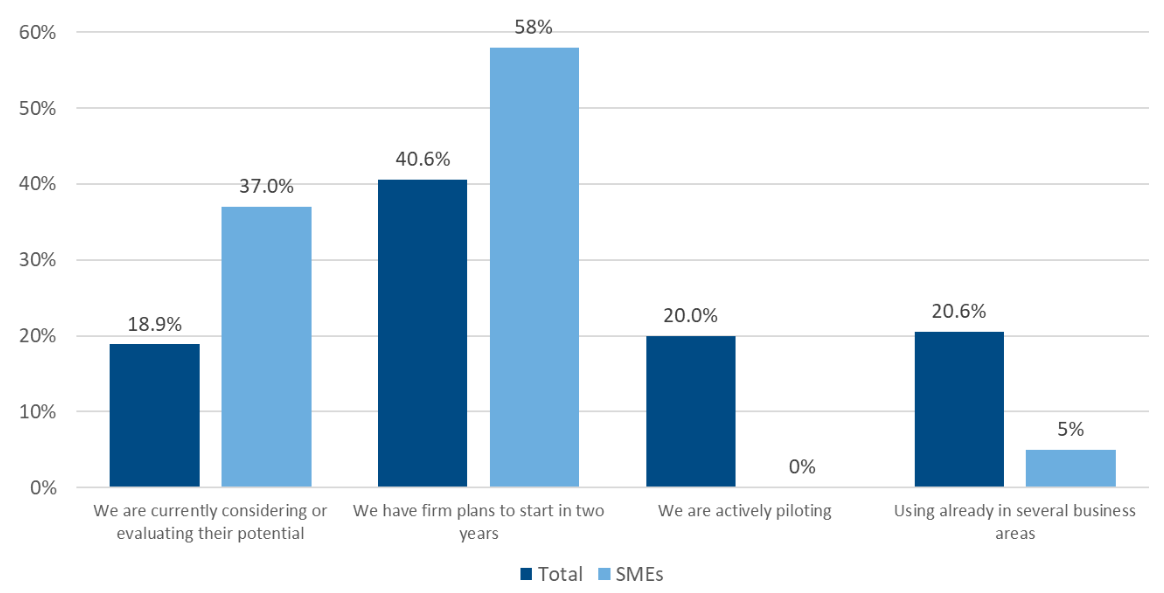
\includegraphics[width = 1\textwidth]{Figuras/AIUse.PNG}
	\end{center}
	\caption{\label{fig:AIBarriers} Uso de servicios/soluciones de IA en Europa (Total de empresas frente a pymes). Fuente: Encuesta de soluciones cognitivas/IA de Europa occidental realizada por IDC, junio 2018 (n = 350).}
\end{figure}

\newpage

Las pymes pueden encontrar una magnífica solución para cumplir con sus necesidades en el Cloud Computing. Los servicios en la nube que ofrecen grandes proveedores como Google, Microsoft o Amazon ponen al alcance de estas empresas la tecnología que antes sólo se podían permitir las grandes organizaciones. Además, al ser recursos completamente gestionados por las empresas proveedoras, las organizaciones pueden centrarse más en su negocio y abstraerse de la infraestructura o la disponibilidad de su sistema. 

La integración de herramientas de IA mediante computación en la nube, en un negocio electrónico, puede ayudar a conseguir los objetivos que persigue la transformación digital. 

La transformación digital lidera un enfoque de negocio centrado en el cliente que busca comprender correctamente los cambios en los comportamientos de los clientes y cómo hacerles llegar los servicios adecuadamente. Se trata además de digitalizar los procesos de negocio y los canales de comunicación, mejorando de esta forma la experiencia de cliente. 

Para entender mejor a los clientes puede resultar muy útil para las organizaciones analizar los sentimientos de los comentarios que éstos publican. En este proyecto se pretende integrar una herramienta que permita llevar a cabo esta acción en una tienda electrónica.

También es muy importante que la empresa garantice una buena experiencia al cliente cuando haga uso de sus servicios. Con esta idea en mente, se quiere además implementar una interfaz conversacional que ayude a ofrecer un servicio más personalizado al consumidor y facilite la navegación por el sitio web a usuarios menos familiarizados con esta plataforma. Este servicio estará disponible en todo momento, aliviando la carga de trabajo de los empleados de atención al cliente. No se debe olvidar que este departamento es la cara visible de la organización e influye directamente sobre la satisfacción de los clientes.

Por último, se persigue asegurar la disponibilidad de estas herramientas y de la propia tienda electrónica haciendo uso de la tecnología de contenerización en la nube.

\section {Objetivos del proyecto}

Este trabajo tiene por objetivo general comprobar el funcionamiento de la Inteligencia Artificial como herramienta de marketing digital en una web. 

Con este fin se creará un portal de comercio electrónico donde se integrarán un servicio de análisis de sentimientos y un bot conversacional. Asimismo, la solución será desplegada en la nube utilizando contenedores.

Los objetivos específicos de este proyecto son:
\begin{itemize}
    \item Aprender a usar los servicios de la nube relacionados con IA y machine learning.
    \item Aprender a diseñar una aplicación con una arquitectura basada en microservicios. 
    \item Aprender a implementar una arquitectura cliente-servidor.
    \item Aprender a desplegar una aplicación en la nube. 
    \item Aprender a utilizar contenedores para el despliegue y desarrollo de una aplicación.
    \item Demostrar la utilidad y escalabilidad de los sistemas basados en cloud.
\end{itemize}

\section {Organización del trabajo}

El trabajo está dividido en siete capítulos que guiarán al lector a través de todo el proceso de desarrollo de la solución propuesta. En este primer capítulo se ofrece una visión general del problema que se pretende resolver y se plantean los objetivos a alcanzar.

\newpage
 
En el segundo capítulo se persigue contextualizar el trabajo describiendo las diferentes áreas de estudio relacionadas con el mismo. Se divide en cinco secciones. En la primera sección se tratará la situación actual de la computación en la nube y se presentarán sus principales características, así como los modelos de servicio más habituales. La segunda sección está destinada a definir el concepto de comercio electrónico y sus principales categorías. Además, se discutirá sobre el presente y futuro de este campo. En la tercera sección, se expondrán los beneficios de aunar computación en la nube y comercio electrónico.

La cuarta sección describe cómo la inteligencia artificial ha dejado de ser una herramienta al servicio de unas pocas organizaciones para convertirse en un recurso accesible a la mayoría de empresas gracias los servicios de computación en la nube.

La quinta sección se ocupa del análisis de sentimientos, se intentará aclarar en qué consiste y  cómo puede ayudar a las empresas. También se presentarán otras aplicaciones más allá de los usos comerciales. Por último, se establecerá una comparación entre algunos de los servicios cloud de análisis de sentimientos más importantes. De forma similar, en la sexta sección se hablará sobre el concepto de interfaz conversacional, ofreciendo una visión de la evolución que ha sufrido esta tecnología hasta la fecha y tratando algunas de las ventajas de su aplicación al comercio electrónico. Se finalizará comparando diferentes herramientas cloud que permiten desarrollar una interfaz de este tipo.

En el tercer capítulo se definirán las etapas en las que de ha dividido el proyecto, ofreciendo una breve explicación sobre cada una de ellas. Igualmente, se comparará la estimación de horas planteada antes de comenzar con el proyecto y los tiempos reales invertidos.

En el cuarto capítulo se propone la solución escogida. Está compuesto por cinco secciones. En la primera sección es donde se realiza un análisis de esta solución, pero sin tener en cuenta aspectos de la implementación. Simplemente, se trata de explicar la idea que se pretende desarrollar y cómo se planea llevarla a cabo. Dicha solución estará formada por tres elementos principales: página web, análisis de sentimientos e interfaz conversacional. En la segunda sección se detallarán los casos de uso del sistema, incluyendo un diagrama de casos de uso, la especificación de los actores y la de cada uno de los casos de uso. La tercera y cuarta sección están incluirán un análisis de requisitos, funcionales y no funcionales, respectivamente.
Para finalizar este capítulo, en la cuarta sección se realizará un estudio económico del proyecto, detallando las tarifas de cada uno de los servicios en la nube y los costes directos e indirectos en los que incurre la realización del proyecto.

En el quinto capítulo se enumerarán las diferentes herramientas utilizadas para el desarrollo del proyecto y se dará información sobre su utilidad. Se ha obviado mencionar aquellas herramientas relacionadas con la realización de la memoria. 
\newpage
El capítulo seis es el eje central del trabajo. Se divide en tres secciones. En la primera sección se explicará la arquitectura del sistema desarrollado. En la segunda sección se realizará un descripción pormenorizada del proceso de implementación para la página web, la herramienta de análisis de sentimientos y la interfaz conversacional. Asimismo, la tercera sección se ocupa de realizar una explicación similar destinada a exponer como desplegar estos componentes en la nube, para lo que se hará uso de contenedores. 

Por último, en el capítulo siete se valorarán los resultados obtenidos tras haber completado el proyecto. Este capítulo consta de dos secciones. En la primera sección se reflexionará sobre los conocimientos adquiridos por el alumno. En la segunda sección se plantearán posibles líneas de trabajo futuro con las que poder continuar mejorando el proyecto.
\chapter{Estado del arte} 
\label{sec:arte}

\section{Computación en la nube}

\begin{flushright}
\begin{minipage}[b][4cm][t]{11cm}
\begin{flushright}
{\small \emph{Si alguien me pregunta qué es la computación en la nube,}} \vspace{-1pt} \\
{\small \emph{trato de no complicarme con las definiciones.}} \vspace{-1pt} \\
{\small \emph{Les digo que, simplemente, la computación en la nube es una}} \vspace{-1pt}\\
{\small \emph{manera mejor de gestionar su negocio.}} \vspace{1mm}\\
{\footnotesize Marc Benioff,} \vspace{-1.5pt} \\
{\footnotesize fundador y presidente de Salesforce.\phantom{l}}
\end{flushright}
\end{minipage}
\end{flushright}

La computación en la nube es un recurso del que pueden disponer las empresas para cumplir con sus necesidades y objetivos. Especialmente para los pequeños negocios, se trata de una herramienta con gran potencial. Debido al elevado grado de globalización todas las empresas del sector del comercio electrónico deben ser competitivas y proveer incentivos que las hagan más atractivas que sus competidores. La computación en la nube puede ayudar a las empresas a incorporar nuevas funcionalidades en su sitio web o aplicación, obteniendo un valor comercial a partir de ellas \cite{Azad2016ImprovementOE}. 

La computación en la nube se ha establecido en el presente y futuro de la industria de la tecnología de la información, así como de los negocios \cite{Hashem}. Ha revolucionando la industria IT aportando flexibilidad a las organizaciones permitiendo que solo paguen por los recursos y servicios que utilizan y durante su tiempo de uso. 

De forma resumida, la computación en la nube es un tipo de modelo de prestación de servicios, con acceso en cualquier momento y facturación por uso. Su arquitectura tiene las siguientes características básicas:

\begin{itemize}
    \item \textbf{Elasticidad}. La habilidad de escalar hacia arriba o abajo las necesidades de computación según los requisitos del cliente.
    \item \textbf{Conectividad}. Permitir el acceso a los servicios a cualquier hora desde cualquier lugar.
    \item \textbf{Visibilidad}. Ofrecer a los consumidores visión y control de los parámetros de despliegue del servicio, uso y coste
    \item \textbf{Uso compartido}. La habilidad de compartir almacenamiento físico, memoria y red en el mismo espacio físico para diferentes usuarios.
    \item \textbf{Medición del servicio}. Medir el servicio y establecer la factura según esos parámetros.
\end{itemize}

La computación en la nube posee una serie de características positivas para hacer frente al rápido crecimiento de las economías y barreras tecnológicas. Permite a las organizaciones centrarse en el negocio principal sin preocuparse por otros problemas como pueden ser la infraestructura, la flexibilidad y la disponibilidad de recursos.

Los modelos de servicio de computación en la nube más comunes hoy en día son PaaS, SaaS, IaaS, CaaS y FaaS. Cada tipo de servicio está dirigido a unos propósitos y consumidores diferentes. A continuación se enumeran cada uno de estos tipos:

\begin{itemize}
    \item \textbf{Infraestructura como servicio (IaaS)}. El proveedor alquila la infraestructura al consumidor, otorgándole casi la totalidad de su control. Es decir, garantiza el acceso del cliente a los recursos de computación (procesador, RAM, disco duro, entre otros) y a las estructuras de red integradas (cortafuegos, routers, seguridad y copias de seguridad). 
    
    Es el cliente quién selecciona los recursos que necesita para satisfacer sus necesidades. Se trata de un servicio muy flexible, ya que, permite al consumidor ampliar o disminuir los recursos contratados de manera rápida y sencilla siempre que lo necesite.
    
    El proveedor por su parte, es el responsable de garantizar la fiabilidad y la seguridad del sistema, a través del mantenimiento de la infraestructura. El modelo de facturación de este servicio es el pago por uso.
    
    Por tanto, se trata de una herramienta que ofrece grandes ventajas por la desaparición de los costes relacionados con la compra y mantenimiento de hardware. 
    
    \item \textbf{Software como servicio (SaaS)}. También conocido como software bajo demanda, se trata de un servicio que pone a disposición del cliente una aplicación específica lista para ser usada, sin precisar instalación, despliegue o mantenimiento alguno. 
    
    Los usuarios acceden a dicho software a través de un navegador web. Todo está administrado por el proveedor: aplicación, sistema, datos, middleware, sistema operativo, virtualización, almacenamiento y redes. El usuario o bien contrata el servicio o accede a él gratuitamente y hace uso del mismo.
    
    \item \textbf{Plataforma como servicio (PaaS)}. Proporciona un entorno de desarrollo e implementación completo en la nube que permite a los desarrolladores crear aplicaciones y servicios. El consumidor adquiere los recursos que necesita y accede a ellos a través de Internet, pagando tan sólo por el uso que hace de los mismos.
    
    Del mismo modo que IaaS, PaaS también incluye la infraestructura, pero además ofrece otras funcionalidades: middleware, servicios de  inteligencia de negocio, herramientas de diseño y desarrollo, sistemas de gestión de bases de datos, entre otras. PaaS permite a los desarrolladores centrarse únicamente en su trabajo, ya que, soporta todo el ciclo de vida de las aplicaciones web: implementación, compilación, pruebas, administración y actualización.
    
    \item \textbf{Función como servicio (FaaS)}. También conocido como arquitectura \textit{serverless}. Por este término se entiende que las tareas relacionadas con el aprovisionamiento y la gestión de la infraestructura son invisibles para el desarrollador, pero es importante destacar que los servidores siguen existiendo y ejecutando el código.
    
    Las aplicaciones se ejecutan en contenedores sin estado, que se crean en el instante del despliegue y se escalan de forma dinámica, es decir, cuando la demanda disminuye se reduce de forma automática la aplicación.
    
    Este tipo de arquitectura favorece el desarrollo de aplicaciones basadas en microservicios, facilitando el ciclo de vida y la implementación continua. 
    
    \item \textbf{Contenedor como servicio (CaaS)}. Se trata de un servicio intermedio entre el IaaS y el PaaS. Consiste  en un modelo de servicios en la nube que permite a los usuarios implementar y gestionar aplicaciones a través de una forma de virtualización basada en contenedores. 
    
    El proveedor ofrece la plataforma en la que se implementan y gestionan los contenedores, automatizando la administración de la infraestructura. 

\end{itemize}

\newpage

A continuación, se resumen gráficamente las diferencias entre los tipos de servicios cloud:
\begin{figure}[ht]
	\begin{center}
		\includegraphics[width = 0.95\textwidth]{Figuras/Comparación Cloud Computing.png}
	\end{center}
	\caption{\label{fig:differentCloudComputing} Diferencias entre IaaS, CaaS, PaaS, FaaS y SaaS}
\end{figure}

\section{Comercio electrónico}

\begin{flushright}
\begin{minipage}[b][4cm][t]{11cm}
\begin{flushright}
{\small \emph{Cuanto antes eliminemos la "e" de "e-commerce"}} \vspace{-1pt} \\
{\small \emph{y lo llamemos simplemente comercio, mejor.}} \vspace{-1pt} \\
{\footnotesize Bob Willett,} \vspace{-1.5pt} \\
{\footnotesize expresidente de Best Buy International.\phantom{l}}
\end{flushright}
\end{minipage}
\end{flushright}

\vspace{-1cm}

Se entiende por comercio electrónico las transacciones comerciales realizadas digitalmente entre organizaciones y personas. Suelen implicar transacciones que ocurren a través de Internet, la Web y/o dispositivos móviles. Estas transacciones conllevan un intercambio de valor (por ejemplo, dinero) entre organizaciones o individuos a cambio de productos y servicios. El intercambio de valor es importante puesto que sin éste no se produce comercio.

En algunas ocasiones las publicaciones técnicas se refieren al comercio electrónico como negocio electrónico, aunque en algún contexto pueden usarse ambos términos como si fueran sinónimos, conviene marcar la diferencia entre los dos conceptos. El comercio electrónico implica principalmente transacciones de compra y venta que realiza la empresa. El negocio electrónico tiene un enfoque más amplio, que incluye al comercio electrónico, consiste en cómo las empresas aplican la tecnología digital y los medios para mejorar la competitividad de su organización mediante la optimización de procesos internos con canales online y tradicionales para comercializar y suministrar \cite{DigitalBusiness}.

La mayor parte de los académicos comparten la opinión de que el comercio electrónico puede dividirse según la naturaleza de la relación del mercado en \cite{E-commerce2016}:

\begin{itemize}
    \item \textbf{B2B (Business-to-Business)}. Los negocios se centran en vender a otros negocios. Es la forma más grande de comercio electrónico. Por ejemplo: Go2Paper es un mercado externo independiente que sirve a la industria del papel.
    \item \textbf{B2C (Business-to-Consumer)}. Se trata de la categoría más común y discutida de comercio electrónico, donde negocios online intentan vender sus productos a consumidores individuales. Incluye tanto bienes, servicios y contenido online. El ejemplo más claro de este tipo es Amazon.
    \item \textbf{C2C (Consumer-to-Consumer)}. Una forma de que los consumidores se vendan productos o servicios entre ellos, con la ayuda de una plataforma online como Ebay o Etsy. También se pueden destacar empresas como Airbnb o Uber que proporcionan una plataforma similar para servicios como el alquiler de habitaciones o transporte.
    \item \textbf{M-commerce}. Se trata de utilizar dispositivos móviles para realizar transacciones online. Involucra el uso de redes wireless para la conexión con Internet.
    \item \textbf{Social e-commerce}. Implica la utilización  de  las redes sociales para facilitar la compra y venta en línea de productos y servicios. Facebook es el líder de este tipo de comercio. 
    \item \textbf{Local e-commerce}. Se enfoca en atraer al consumidor en función de su localización geográfica actual. Esta forma de comercio electrónico cobra mucha importancia en la actualidad debido a las restricciones de movilidad que se aplican a los ciudadanos en diferentes países del mundo.
\end{itemize}

La situación actual del comercio electrónico está caracterizada por su vertiente social. El contenido de entretenimiento se ha convertido es una de las mayores fuentes de beneficios y el m-commerce se ha instaurado como una realidad con grandes previsiones de crecimiento. El marketing ha sufrido un cambio de paradigma donde se ha sustituido el antiguo marketing transaccional centrado en qué hacer a los clientes por el nuevo concepto de marketing relacional que pone el acento en qué hacer por los clientes \cite{manualGestion}. Las organizaciones han trasladado su presencia online a las redes sociales como Twitter o Instagram, ya que, la gran cantidad de usuarios de estas plataformas suponen una oportunidad de negocio que no debe ser ignorada. Además, han surgido nuevas empresas que han sabido capitalizar activos no utilizados como automóviles o habitaciones libres, tales como Airbnb o Uber \cite{E-commerce2016}. 

En un estudio que la empresa Cetelem realizó sobre el comercio electrónico en España, cuando Miguel Hernández Granado, director de producto para Lenovo en España y Portugal, fue preguntado por la situación actual del comercio electrónico en España, éste respondió: "De los últimos estudios acerca del tema se desprende la idea general de que el sector del comercio electrónico en España está en el buen camino. Tan solo en 2018, el e-commerce rozó en nuestro país los 40.000 millones de euros, lo que supone un incremento del 29\% en comparación con el año anterior, según datos de la Comisión Nacional de los Mercados y la Competencia. Las previsiones de crecimiento y expectativas son favorables e, incluso, aun cuando se espera un descenso en las ventas con relación al ejercicio anterior. Esta tendencia optimista está claramente auspiciada por la madurez del sector y la cada vez mayor normalización de la compra online por parte de los consumidores. España en los próximos años será uno de los países que más crecimiento en e-commerce tendrá en Europa" \citeW{granado}. 

En la siguiente figura se puede observar el crecimiento que experimentaría, antes del Covid-19, el sector del comercio electrónico en España para 2023:

\begin{figure}[ht]
	\begin{center}
		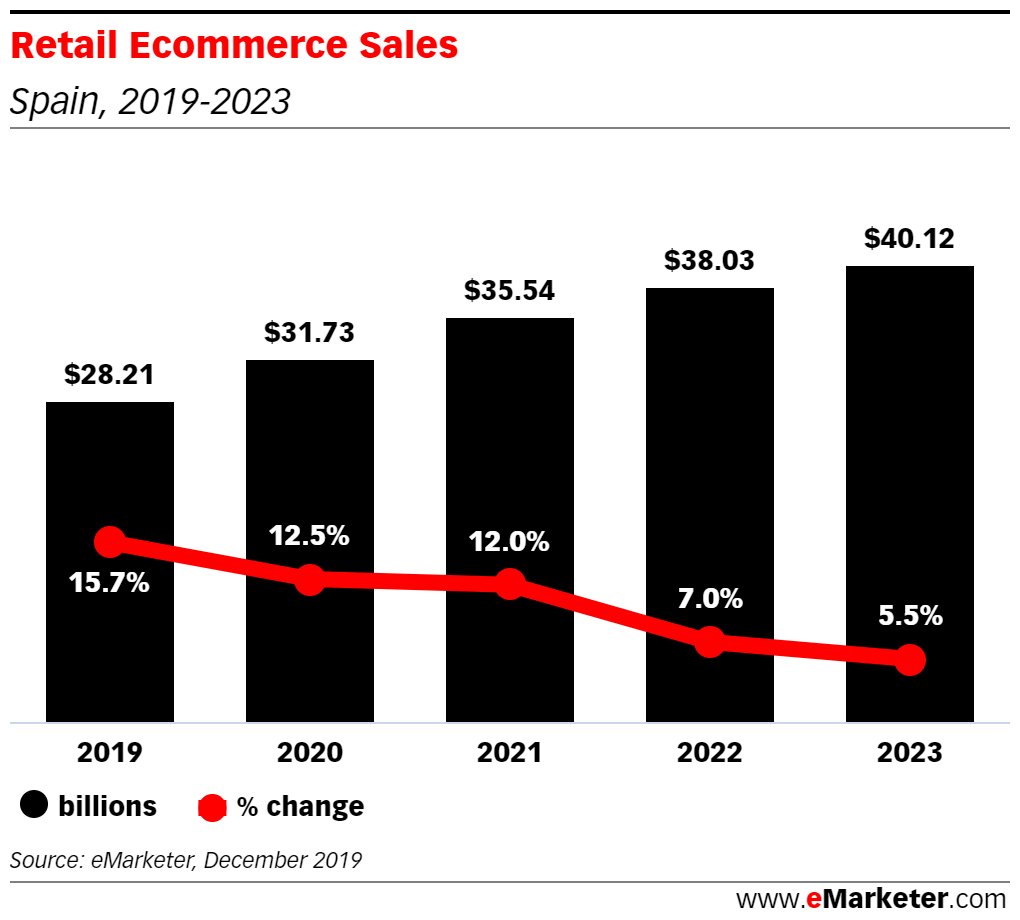
\includegraphics[width = 0.50\textwidth]{Figuras/ecommerce-españa-crecimiento-predicción-.png}
	\end{center}
	\caption{\label{fig:retailSpain} Ventas minoristas de comercio electrónico en España. Fuente: eMarketer.}
\end{figure}

\newpage

La pandemia ha supuesto un duro golpe para el comercio minorista español, se prevee una caída del 12,7\% este año frente a un pronóstico previo de crecimiento del 1,9\%. Sin embargo, ha repercutido positivamente en las previsiones para el comercio electrónico. Se espera que se alcance un total de 32.89 billones de dólares y que continúe aumentando hasta los 41.73 billones en 2023 \citeW{emarketerSpain}. 

Antes de la situación generada por el coronavirus también se esperaba un crecimiento del sector del comercio electrónico a nivel global, como se muestra a continuación:

\begin{figure}[ht]
	\begin{center}
		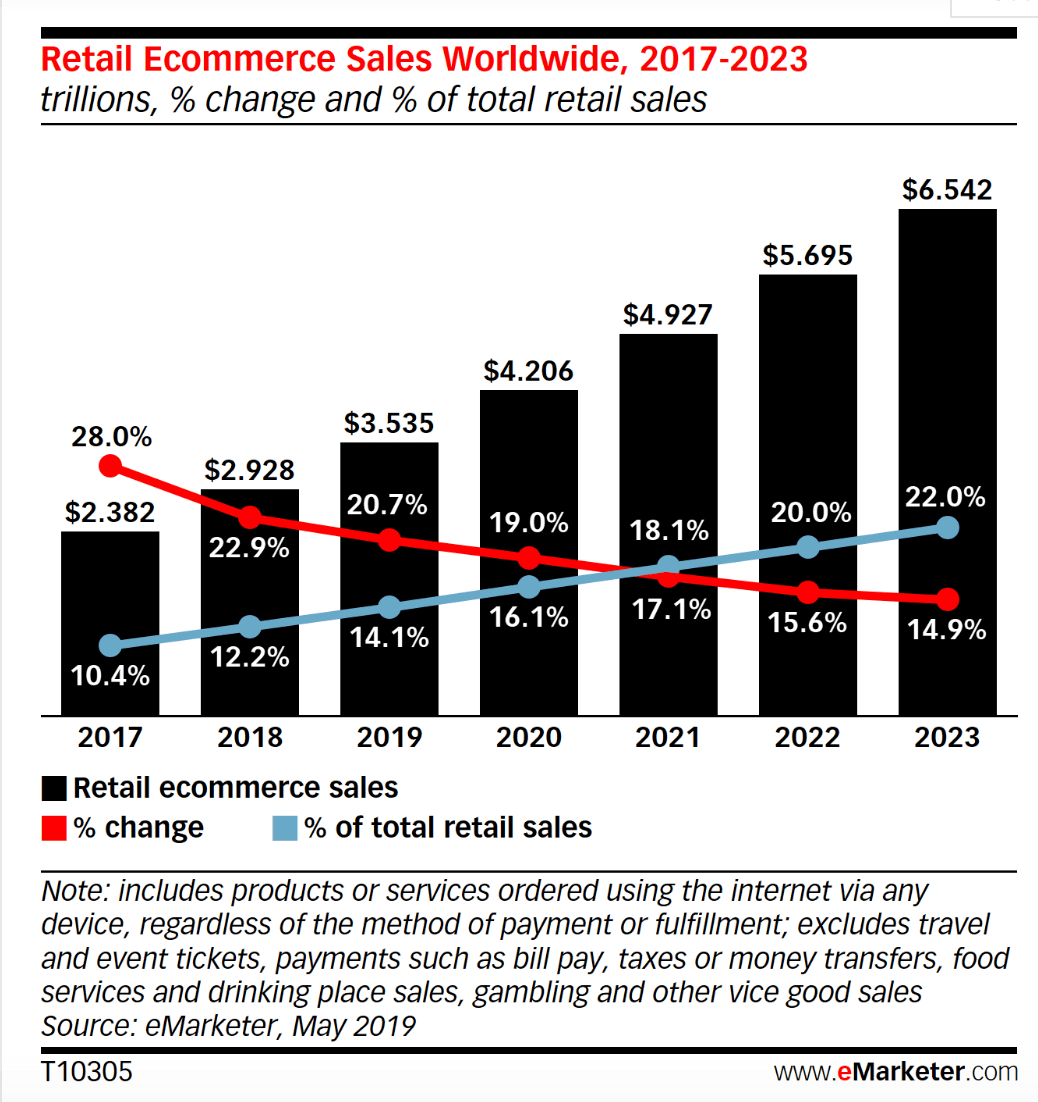
\includegraphics[width = 0.55\textwidth]{Figuras/Global-online-retail-e-commerce-growth.png}
	\end{center}
	\caption{\label{fig:retailWorldwide} Ventas minoristas de comercio electrónico en el mundo. Fuente: eMarketer.}
\end{figure}

A causa de las cuarentenas y los cierres de negocios que están experimentando los consumidores alrededor del mundo, el comercio electrónico se ha convertido en una excelente alternativa de conseguir productos básicos. Este año se espera una tasa de crecimiento  del 16,5\% para el comercio electrónico lo que supone una caída del 3,7\% respecto al pronóstico anterior del 20,2\%. Esta caída será más acentuada en el resto de ventas, un 10\% respecto a las previsiones anteriores \citeW{emarketerGlobal}. 

\newpage

\section{Computación en la nube y comercio electrónico}

La computación en la nube tiene una gran cantidad de connotaciones positivas sobre el comercio electrónico. La ventaja principal es que permite a las empresas reducir en gran medida los costes que supone construir y mantener una página web porque la infraestructura de hardware y software necesaria se puede contratar a un proveedor cloud, pagando tan sólo por el uso que se haga del servicio. Existen otros puntos a favor de esta tecnología \cite{SME}:

\begin{itemize}
    \item \textbf{Escalabilidad}. Se pueden adaptar rápidamente los recursos de los que se hace uso en función de las necesidades del negocio.
    \item \textbf{Disponibilidad y movilidad}. Los usuarios pueden acceder a los productos y servicios de la empresa en cualquier lugar y en cualquier momento. 
    \item \textbf{Foco en el negocio}. Las organizaciones pueden centrarse en la actividad de su negocio y abstraerse de la infraestructura.
    \item \textbf{Administración sencilla}. Convierten el mantenimiento de la infraestructura hardware y software en un proceso más sencillo.
    \item \textbf{Control de desastres}. En el caso de que se produzca un desastre las empresas pueden restablecer su actividad en un período corto de tiempo, ya que toda la infraestructura hardware y software no habrá sufrido daño alguno.
    \item \textbf{Seguridad}. Los proveedores más importantes de servicios cloud garantizan la seguridad de los datos almacenados en sus plataformas.
\end{itemize}

El objetivo último de todas las empresas al adoptar la tecnología cloud es aumentar su competitividad, aunque esta acción por sí misma no garantizará el éxito. Se debe considerar tan sólo como un escalón más en el establecimiento del negocio.

\newpage

\section{Democratización de la IA}

\begin{flushright}
\begin{minipage}[b][4cm][t]{11cm}
\begin{flushright}
{\small \emph{Ya no necesita un presupuesto multimillonario }} \vspace{-1pt} \\
{\small \emph{para introducir la IA en su empresa. }} \vspace{-1pt} \\
{\small \emph{La IA representa una oportunidad para }} \vspace{-1pt} \\
{\small \emph{las empresas más pequeñas de }} \vspace{-1pt} \\
{\small \emph{competir en igualdad de condiciones.}} \vspace{1mm}\\
{\footnotesize Nichole Jordan,} \vspace{-1.5pt} \\
{\footnotesize socio director en Grant Thornton LLP.\phantom{l}}
\end{flushright}
\end{minipage}
\end{flushright}

En un contexto empresarial, se entiende por democratización de la inteligencia artificial hacer que ésta sea accesible para todas las organizaciones. En el pasado siglo se alcanzó una cima de democratización de los recursos tecnológicos, el futuro de la tecnología para las próximas décadas es la Inteligencia Artificial: usar hardware y software para reconocer patrones, hacer predicciones, aprender y mejorar, y tomar medidas basadas en ella. Los más optimistas ven a la IA como una herramienta positiva, que puede ayudar a cada persona a lograr más y mejor.

Gigantes como Google, Amazon, Microsoft, Apple y Facebook son  muy conscientes del poder transformador que conlleva la aplicación de la IA. El aprendizaje profundo es la base del sistema de recomendaciones de Amazon, las herramientas de búsqueda y traducción de Google y el asistente personal Cortana de Microsoft, así como muchas otras aplicaciones y servicios ampliamente utilizados. La mayoría de las empresas que se encuentran entre las 500 más ricas del mundo también tienen equipos dedicados a la IA. El interés de estas grandes fortunas ha agotado los profesionales dedicados a la ciencia de datos, lo que hace especialmente costoso para las pymes la contratación de científicos de datos cuando intentan introducirse en este campo.

Incluso aquellas empresas que pueden permitirse el lujo de contratar a expertos en inteligencia artificial todavía necesitan preparar grandes conjuntos de datos y realizar una fuerte inversión económica en potencia informática para analizarlos y enseñar a su red neuronal a reconocer ciertos patrones u objetos. Sin embargo, los grandes proveedores de la nube se han percatado de los problemas de esta situación y creen que han encontrado una manera de ayudar a las personas a superarlos.

En la actualidad, el aprendizaje automático como servicio, o IA en la nube, se ha convertido en un componente importante de las plataformas como Amazon Web Services (AWS), Microsoft Azure, Google Cloud e IBM Cloud. En esencia, estas compañías ofrecen a sus clientes modelos de aprendizaje profundo previamente entrenados, de modo que puedan ser incorporados por aplicaciones comerciales, por ejemplo, para el reconocimiento de imágenes, así como herramientas que simplifican el proceso de construcción, capacitación y despliegue de modelos personalizados en la nube \citeW{democratizingAI}. 

Con las grandes empresas tecnológicas muy por delante del resto, la industria se pregunta si las pymes realmente pueden beneficiarse de la IA, y transformarse.

\section{Análisis de sentimientos}

\begin{flushright}
\begin{minipage}[b][4cm][t]{11cm}
\begin{flushright}
{\small \emph{Nadie lo expresa así, pero creo que la inteligencia artificial  }} \vspace{-1pt} \\
{\small \emph{es casi una disciplina humanística. }} \vspace{-1pt} \\
{\small \emph{En realidad supone un intento de comprender  }} \vspace{-1pt} \\
{\small \emph{la inteligencia y la cognición humanas.}} \vspace{1mm}\\
{\footnotesize Sebastian Thrun,} \vspace{-1.5pt} \\
{\footnotesize fundador de Udacity.\phantom{l}}
\end{flushright}
\end{minipage}
\end{flushright}

\vspace{-10pt}

Los científicos llevan muchos años intentando imitar la mente humana mediante sistemas "inteligentes". Desde que John McCarthy y Marvin Minsky fundaran la Inteligencia Artificial en 1956 se han conseguido resultados, inimaginables en ese entonces, que han demostrado la utilidad social, intelectual y cultural que tiene para la sociedad esta tecnología. Actualmente, resulta muy sencillo enseñar a una IA a ganar una partida de ajedrez, en cambio, el reto está en conseguir que pueda emular un sistema tan complejo como la mente humana. Como dijo Alan Winfield, profesor de robótica en la UWE (Bristol): "Hoy en día hemos aceptado que, 60 años más tarde del nacimiento de la IA, las cosas que originalmente asumíamos como fáciles, en realidad han resultado ser muy difíciles y lo que pensábamos que era difícil, como jugar al ajedrez, es en realidad muy fácil" \citeW{luca}.

La inteligencia emocional es una capacidad inherente al ser humano, si bien es cierto que algunas personas son más sensibles, todas pueden interpretar las emociones y los sentimientos del resto. Por tanto, ¿es posible enseñar esta capacidad a una máquina?

Con esta idea en mente surgió la Computación Afectiva, una rama de la IA destinada a procesar, comprender y replicar las emociones humanas. Este campo data al menos del 1995 cuando Rossalin Picard, profesora en el MIT, publicó "Affective Computing" \cite{picard1995}.


Para las máquinas, al igual que el ser humano, resulta más sencillo obtener información sobre las emociones a partir de un vídeo o una conversación hablada. El análisis de sentimientos, un subcampo del procesamiento del lenguaje natural, se ocupa de identificar opiniones, emociones y evaluaciones positivas o negativas respecto a diferentes temas \cite{polarity}. En este sentido la Inteligencia Artificial tiene una serie de obstáculos por delante, ya que, la comunicación humana va acompañada de principios difíciles de recrear artificialmente como son el humor, los dobles sentidos, la ironía o los sentimientos que añade el comunicador.

Analizar el sentimiento de una unidad de texto puede abarcar tanto la opinión como la emoción detrás de esa unidad. En la siguiente oración se puede observar fácilmente la diferencia entre opinión y emoción: "Pienso que he tomado la decisión adecuada al mudarme a Berlín, aunque me siento triste por estar lejos de mi familia". Esta frase expresa una opinión positiva y una emoción negativa sobre el mismo tema. El análisis de opiniones está más relacionado con determinar si la expresión es positiva, negativa o neutral, mientras que el de emociones se encarga del estudio del sentimiento reflejado en el fragmento de texto (tristeza, alegría, rabia, odio, etc.) \cite{curentStateSentiment}. 

A lo largo del trabajo se utilizarán los términos análisis de sentimientos o análisis de opiniones para hacer referencia a este campo de estudio, ya que su uso está generalizado en el mundo académico.

Las opiniones que los consumidores publican en Internet sobre los productos que han adquirido tienen un gran impacto, pues muchos usuarios las utilizan para tomar la decisión de adquirir un producto o servicio. Además, también importan a las empresas, puesto que quieren conocer que piensan los clientes sobre sus productos y servicios. Se han realizado una gran cantidad de estudios en este sentido:
\begin{itemize}
    \item Según un estudio publicado en 2017 por la plataforma online Podium, donde se realizó una encuesta a 2005 consumidores estadounidenses \citeW{Podium}:
    \begin{itemize}
        \item El 93\% de los consumidores afirma que las opiniones que leen en línea afectan a sus decisiones de compra.
        \item 3.3 es la calificación mínima de estrellas para que los consumidores realicen una compra.
    \end{itemize}
    \item Un aumento de una estrella en la calificación de Yelp conduce a un incremento del 5 al 9\% en los ingresos. Yelp es una aplicación web y móvil que permite a los usuarios conocer las opiniones y calificaciones que otros usuarios han publicado sobre negocios y sus servicios. Esta conclusión ha sido obtenida por un estudio realizado por Michael Luca para Harvard Business School \cite{yelp}.
    \item Las empresas corren el riesgo de perder hasta el 22\% de los clientes cuando éstos encuentran un sólo artículo negativo sobre el producto que van a comprar; si aparecen tres en la búsqueda, el potencial de pérdida de clientes aumenta al 59,2\%. Estos datos se han extraído de una encuesta realizada por la plataforma Moz, donde se preguntó a 1000 consumidores sobre sus interacciones con Google y otras plataformas durante el proceso de compra.
    \item Según datos ofrecidos por Google en una encuesta realizada a 14096 consumidores alrededor del mundo: el 59\% de los compradores encuestados afirman que investigan en internet antes de llevar a cabo una compra \citeW{thinkGoogle}.
\end{itemize}

Los usos comerciales más comunes del análisis de sentimientos son \cite{mejova}:
\begin{itemize}
    \item Seguimiento de opiniones de usuarios y calificaciones de productos y/o servicios.
    \item Análisis de tendencias de consumo, competidores y mercado.
    \item Medición de la respuesta de los usuarios a incidentes relacionados con la empresa.
    \item Prevención de efectos virales negativos.
    \item Valoración de comentarios en diferentes idiomas.
\end{itemize}

Además de los intereses comerciales, el uso de este tipo de aplicaciones se está extendiendo en organismos gubernamentales. Los gobiernos monitorean las redes sociales para descubrir sentimientos y preocupaciones de los ciudadanos. Este hecho es especialmente reseñable en China \cite{sentimentAnalysis}. 

También se han publicado muchos trabajos de investigación orientados a diversas aplicaciones del análisis de sentimientos. Algunas de éstas se han centrado en el análisis de opiniones sobre productos y películas (Hu y Liu, 2004 \cite{hu2004}; Popescu y Etzioni, 2005 \cite{popescu}). Estos textos cuentan con la ventaja de que ya tienen un tema claramente especificado. Muchos investigadores también han analizado las opiniones públicas durante una campaña electoral, como Chung y Mustafaraj (2011) \cite{twitterPolitical} y Gayo-Avello et al. (2011) \cite{gayo-avello} que discuten sobre las limitaciones de utilizar datos obtenidos de Twitter para predecir las elecciones políticas. Otra área popular de aplicación es la predicción del mercado de valores. Por ejemplo, Zhang et al. (2010) \cite{zhanget} identifica estados de ánimo positivos y negativos en Twitter y hace uso de esta información para predecir el movimiento de los índices bursátiles.

Actualmente, como se ha mencionado en la sección 2.4, el procesamiento del lenguaje natural se ha convertido en un elemento importante dentro de las plataformas cloud más destacadas. Algunos de los servicios disponibles son:

\begin{itemize}
    \item \textbf{Google Cloud Natural Language}. Permite la detección de idiomas, el análisis de opiniones, el análisis de entidades, el análisis de opiniones sobre entidades, la clasificación de contenido y el análisis sintáctico. El análisis de un texto mediante esta herramienta da como resultado dos valores numéricos \citeW{googleNaturalLanguage}:
    \begin{itemize}
        \item Puntuación. Número decimal comprendido entre -1,0 (negativo) y 1,0 (positivo). Se corresponde con la tendencia emocional general del texto.
        \item  Magnitud. Número decimal comprendido entre 1,0 y $\infty$. Expresa la intensidad de la emoción. Se debe considerar que para el cálculo de este valor se tiene en cuenta cada expresión de emoción en el texto, por tanto, los valores de magnitud para textos más largos es probable que sean mayores.
    \end{itemize}
    \begin{lstlisting}[caption= Salida al analizar el sentimiento de un texto con Natural Language]
        {
          "documentSentiment": {
            "magnitude": 0.8,
            "score": 0.8
          },
          "language": "en",
          "sentences": [
            {
              "text": {
                "content": "Enjoy your vacation!",
                "beginOffset": 0
              },
              "sentiment": {
                "magnitude": 0.8,
                "score": 0.8
              }
            }
          ]
        }

    \end{lstlisting}
    \item \textbf{Amazon Comprehend}. Se puede usar para el análisis sintáctico, la extracción y análisis de entidades, la detección de idiomas, la clasificación de contenido y el análisis de opiniones. Analizar los sentimientos de un texto con esta herramienta permite determinar si el sentimiento es positivo, negativo, neutral o combinado. 
    
    Como salida devuelve el sentimiento más probable para el texto y las puntuaciones para cada uno de los sentimientos. La puntuación representa la probabilidad de que el sentimiento se haya detectado correctamente. En el ejemplo que se muestra a continuación existe un 95\% de probabilidad de que el texto exprese un sentimiento positivo y un 1\% de que contenga un sentimiento negativo \citeW{comprehend}.
    
    \begin{lstlisting}[caption=Salida al analizar el sentimiento de un texto con Amazon Comprehend ]
        {
        "SentimentScore": {
                "Mixed": 0.030585512690246105,
                "Positive": 0.94992071056365967,
                "Neutral": 0.0141543131828308,
                "Negative": 0.00893945890665054
            },
            "Sentiment": "POSITIVE",
            "LanguageCode": "en"
        }
    \end{lstlisting}
    \item \textbf{Watson Natural Language Understanding}. Esta herramienta, propiedad de IBM, permite a los usuarios el análisis de opiniones, la detección de idiomas, el análisis de entidades y el análisis de emociones (tristeza, alegría, miedo, rabia y  disgusto). Sin embargo, no cuenta con la funcionalidad de realizar análisis de temas. En cuanto al análisis de opiniones, analiza el sentimiento general del texto y el sentimiento respecto a cada una de las frases que lo componen. Puede realizar este análisis respecto a entidades y palabras clave. Este servicio ofrece como respuesta un número real comprendido entre -1 (negativo) y 1 (positivo) \citeW{watson}. 
    
     \begin{lstlisting}[caption=Salida al analizar el sentimiento de un texto con Watson ]
    {
      "usage": {
        "text_units": 1,
        "text_characters": 1188,
        "features": 1
      },
      "sentiment": {
        "targets": [
          {
            "text": "stocks",
            "score": 0.279964,
            "label": "positive"
          }
        ],
        "document": {
          "score": 0.127034,
          "label": "positive"
        }
    },
    \end{lstlisting}
    
    \item \textbf{Microsoft Azure Language Understanding Intelligent Service (Luis)}. Permite la detección de idiomas, el análisis de opiniones, el reconocimiento y la extracción de entidades.  Evalúa el texto y devuelve las etiquetas y puntuaciones de opinión de cada oración. La puntuación toma un valor entre 0 y 1, representando 1 la opinión más positiva y 0 la más negativa \citeW{luis}. La salida se muestra de la siguiente forma:
    \begin{lstlisting}[caption=Salida al analizar el sentimiento de un texto con Luis ]
    "sentimentAnalysis": {
      "label": "positive",
      "score": 0.9163064
    }
    \end{lstlisting}
\end{itemize}

\newpage

En la siguiente figura se comparan las funcionalidades de estos servicios:
\vspace{-10mm}
\begin{figure}[ht]
	\begin{center}
		\includegraphics[width = 0.95\textwidth]{Figuras/Comparación Cloud Machine Learning.png}
	\end{center}
	\caption{\label{fig:NLPComparative} Comparación servicios NLP}
\end{figure}



\section{Interfaces conversacionales}

\begin{flushright}
\begin{minipage}[b][4cm][t]{11cm}
\begin{flushright}
{\small \emph{Los centros de llamadas, sitios web y aplicaciones móviles}} \vspace{-1pt} \\
{\small \emph{ya no son el único medio de interacción con las marcas.}} \vspace{-1pt} \\
{\small \emph{Los chatbots se están convirtiendo en una necesidad }} \vspace{-1pt}\\
{\small \emph{para las empresas que persiguen un enfoque al cliente. }} \vspace{-1pt}\\
{\small \emph{Este canal de comunicación online ha sido el que más ha crecido.}} \vspace{1mm}\\
{\footnotesize Eileen Brown,} \vspace{-1.5pt} \\
{\footnotesize autora de Social Media Marketing for Business.\phantom{l}}
\end{flushright}
\end{minipage}
\end{flushright}


Una interfaz conversacional es un programa de ordenador diseñado para simular una conversación con uno o más usuarios humanos mediante voz o texto. Se puede programar para mantener conversaciones breves y servir como medio de interacción con los usuarios, proporcionándoles respuestas basadas en preguntas comunes. El sistema entiende el contexto y ofrece una respuesta basada en el mensaje que se le da \cite{Gupta2015AnEW}. 

\newpage

La idea de construir un software capaz de mantener una conversación con los humanos dando la ilusión de una verdadera interacción entre humanos se remonta  a los años 50, cuando Alan Turing propuso su "Juego de imitación" \cite{turing}. Más conocido como Test de Turing, su objetivo es determinar si una máquina puede mantener una conversación con un ser humano sin ser detectada como tal. Hoy en día aún se utiliza este test para evaluar en qué medida un bot es humano. El premio Loebner se asigna cada año al sistema informático que mejor finge ser humano \cite{riseOfBots}.

El primer ejemplo de chatbot se remonta a 1966 cuando Joseph Weizenbaum creó ELIZA \cite{eliza}, un programa que sirvió de ejemplo para demostrar las posibilidades de comunicación entre humano y ordenador a través del lenguaje natural. ELIZA interpretaba el papel de un psicoterapeuta y se dedicaba a responder vagamente a las peticiones del usuario, trabajaba sobre la base de un diccionario estructurado y buscaba palabras claves en el texto. ELIZA sentó las bases de los bots durante los siguientes 50 años, hasta hoy en día.

Especialmente en los últimos años, los bots han cobrado importancia debido a los grandes avances en inteligencia artificial, plataformas, dispositivos de comunicación y reconocimiento de voz \cite{peterAI}; han ganado más capacidades y "residen" en la nube.

Hasta la fecha, los clientes que querían contactar con una empresa tenían que completar formularios o realizar una llamada, lo que a menudo implica largos tiempos de espera. Este tipo de comunicación tiende a ser unitaleral, molesto y lento para los clientes. Por otro lado, la comunicación con amigos, conocidos y familiares se realiza cada vez más a través de plataformas de mensajería como WhatsApp, Telegram, Facebook Messenger, etc. En este contexto, se puede observar que las empresas están adoptando un nuevo paradigma de comunicación en el que hacen uso de plataformas de mensajería, chatbots y algoritmos para contactar con los clientes. 

Este paradigma de comunicación ha hecho surgir nuevas tendencias como:
\begin{itemize}
    \item Comercio conversacional. Asesoramiento al cliente y compra a través de una conversación.
    \item Asistentes personales. Asistentes personales digitales que se hacen cargo de las compras, reservas y planificación para el usuario.
    \item Marketing algorítmico. Integración de algoritmos y bots publicitarios en todos los pasos del proceso de marketing.
    \item Oficina conversacional. Integración de plataformas de mensajería combinadas con bots en procesos internos de la compañía.
\end{itemize}


Dada la gran cantidad de personas que utilizan aplicaciones de mensajería, resulta lógico que las empresas empiecen a ofrecer sus servicios mediante esos medios. En lugar de convencer a los clientes para que se instalen una nueva aplicación, resulta más efectivo para las empresas reunir a sus clientes donde ya se encuentran, pues el chat ya está integrado en sus vidas diarias. 

La aplicación de estas tendencias al comercio electrónico da como resultado procesos más eficientes, mayor retención de clientes, un aumento en las ventas y una ventaja competitiva respecto a otras empresas. Para los clientes, aumenta considerablemente la comodidad, ya que, incluso las tareas más molestas pueden resolverse en cuestión de minutos. Si las organizaciones no se adaptan a las nuevas tendencias puede darse la situación de que los consumidores no tengan en cuenta sus productos o servicios en el futuro. \cite{peterAI}.

En cuanto a los sitios web de comercio electrónico actuales, éstos contienen una amplia gama de productos ordenados por categorías, dando como resultado una base de datos enorme y compleja. La navegación por estas páginas para localizar los productos deseados, de acuerdo con las especificaciones del consumidor, puede ser un proceso poco intuitivo, lento y exasperante \cite{Gupta2015AnEW}. Las herramientas de búsqueda no ofrecen resultados adecuados cuando se utilizan palabras ambiguas e imprecisas para describir un producto. Además, si un usuario no tiene mucho conocimiento sobre el producto que pretende comprar, los sistemas convencionales tampoco ayudan mucho. \cite{Gupta2015AnEW}. 
 
La implementación de un chatbot en el portal de comercio electrónico sirve para resolver esta problemática ofreciendo una forma más intuitiva de interactuar con el sitio web.

En la actualidad, los principales proveedores de servicios cloud cuentan con su propio motor conversacional para llevar a cabo el desarrollo de un chatbot. A continuación se presentan estas herramientas:

\begin{itemize}
    \item \textbf{Dialogflow}. Esta tecnología, perteneciente a Google, ofrece la posibilidad de crear agentes conversacionales dedicados a mantener conversaciones con los usuarios. Ante la entrada de una petición, la interpretan y da una respuesta previamente programada. A través del intercambio de información van perfeccionando sus conocimientos.
    
    Se puede integrar con hasta dieciséis plataformas diferentes, entre las que destacan: Twitter, Facebook, Slack y Alexa. Además, a partir de la API de Dialogflow se puede integrar en otras aplicaciones aparte de esas. Puede funcionar en veinte idiomas distintos. Tiene tres versiones, dos de pago y una gratuita. Esta última ya incluye todas las características principales para los desarrolladores.

    \item \textbf{Amazon Lex}. Este servicio, proporcionado por Amazon, permite la construcción de chatbots para cualquier aplicación o dispositivo que use voz y texto. Con Amazon Lex, cualquier desarrollador puede crear bots conversacionales al instante.
    
    Amazon Lex proporciona funcionalidades avanzadas de deep learning como el reconocimiento de voz automático (ASR) para convertir el habla en texto y la comprensión del lenguaje natural (NLU) para reconocer la intención del texto. Sólo acepta el inglés estadounidense lo que puede suponer una desventaja. Ofrece a los desarrolladores un año de prueba gratuito tras el cuál se puede continuar haciendo uso del servicio adhiriéndose a un plan de pago en el que se cobra por petición realizada.
    
    \item \textbf{Luis}. Se trata de la misma herramienta que ya se vió en la sección anterior. Luis interpreta el mensaje introducido por el usuario y obtiene información importante que utiliza para ofrecer una respuesta preprogamada. Una de las características clave de Luis es la tecnología de aprendizaje activo. Una vez que el bot comienza a funcionar continúa aprendiendo y permite la actualización constante. Ofrece dominios preconstruidos para dispositivos, música, calendario, etc. Admite hasta trece idiomas y se puede integrar en plataformas como Cortana, Microsoft Teams, Facebook, Slack o Skype. 
    
    En cuanto a los planes de pago, cuenta con un modo gratuito que permite realizar hasta 10000 peticiones mensuales y un máximo 5 peticiones por segundo. El plan de pago básico acepta hasta 10 transacciones por segundo y cobra 0,75\$ por cada 1000 peticiones.
    
    \item \textbf{IBM Watson}. Es una herramienta de inteligencia artificial desarrollada por IBM. Trabaja todas las formas de datos, interactuar con las personas y aprender de esa interacción. IBM trasladó la tecnología de Watson a la nube y lanzó esta API, que permite al usuario construir sus propios bots conversacionales. Al igual que el anterior, pone a disposición del usuario dominios preconstruidos de atención al cliente, banca, utilidades, comercio electrónico, entre otros temas. Acepta trece idiomas diferentes y se puede integrar prácticamente en cualquier plataforma de mensajería. Posee cuatro modos de pago. El más básico es gratuito y permite realizar 1000 peticiones cada mes; el estándar supone un coste de 0,0025\$ por llamada pero no tiene límites. Para obtener información sobre los otros dos hay que contactar con IBM.
    
\end{itemize}
\chapter{Etapas de desarrollo} 
\label{sec:fases}

El desarrollo de este proyecto se divide en cinco etapas generales:
\begin{enumerate}
    \item \textbf{Etapa de análisis}. Se hará un estudio de los objetivos a alcanzar y las tecnologías con las que se llevarán a cabo. Se pretende conseguir una idea clara y precisa sobre las tareas a realizar en etapas posteriores. 
    \item \textbf{Etapa de implementación web}. Se realizará la implementación de un sitio web para un negocio ficticio. Dicha página será la base sobre la que se trabajará en las siguientes etapas.   
    \item \textbf{Etapa de implementación de los servicios}. Se integrarán dos servicios bien diferenciados en la página de comercio electrónico:
        \begin{enumerate}
            \item Análisis de sentimientos. Con el objetivo de implementar este servicio se utilizará la herramienta NLP (Natural Language Processing), ofrecida por la plataforma de Google Cloud. Para ello, es necesario desarrollar un cliente que actúe como intermediario entre la página web y la llamada a NLP. Esta aplicación funcionará como una especie de envoltorio sobre la API (Application Programming Interface) original.
            \item Bot conversacional. Se desarrollará usando el servicio DialogFlow de Google y, posteriormente, se integrará en la página web.
        \end{enumerate}
    \item \textbf{Etapa de despliegue}. Se utilizarán contenedores para desplegar el sistema en una plataforma sin servidor.
    \item \textbf{Etapa de evaluación}. Se procederá a comprobar el correcto funcionamiento de la página web y las herramientas integradas.
\end{enumerate}

\newpage

Cada una de las etapas se ha dividido en diferentes tareas, de forma que a cada tarea se le ha asignado una fecha de inicio y de fin, así como el número de horas que se espera invertir para su realización. En la siguiente tabla se presenta la planificación temporal prevista para la realización del proyecto:


\begin{table}[!ht]
  \centering
    \scalebox{0.85}[0.85] {
    \begin{tabular}{lcccc}
    \toprule
    \multicolumn{1}{c}{\textbf{ACTIVIDAD}} & \textbf{FECHA INICIO} & \textbf{DURACIÓN  } & \textbf{FECHA FIN } & \textbf{HORAS} \\
    \midrule
    PROYECTO & 01/02/2020 & 111   & 22/05/2020 & 300 \\
    \midrule
      ANÁLISIS & 01/02/2020 & 29    &  01/03/2020 & 40 \\
    \midrule
        Estudio del problema & 01/02/2020 & 15    & 16/02/2020 & 10 \\
    \midrule
        Requisitos & 01/02/2020 & 29    &  01/03/2020 & 15 \\
    \midrule
        Herramientas & 01/02/2020 & 29    &  01/03/2020 & 15 \\
    \midrule
      IMPLEMENTACIÓN WEB & 02/03/2020 & 15    & 17/03/2020 & 30 \\
    \midrule
        Crear Wordpress & 02/03/2020 & 3     & 05/03/2020 & 2 \\
    \midrule
        Introducir productos & 06/03/2020 & 3     & 09/03/2020 & 5 \\
    \midrule
        Introducir opiniones & 06/03/2020 & 3     & 09/03/2020 & 3 \\
    \midrule
        Diseño & 10/03/2020 & 2     & 12/03/2020 & 10 \\
    \midrule
        Desarrollo de componentes & 13/03/2020 & 4     & 17/03/2020 & 10 \\
    \midrule
      IMPLEMENTACIÓN DE SERVICIOS & 18/03/2020 & 53    & 10/05/2020 & 130 \\
    \midrule
        Desarrollo APIs propias & 18/03/2020 & 18    & 05/04/2020 & 40 \\
    \midrule
        Conexión Google NLP  & 06/04/2020 & 6     & 12/04/2020 & 10 \\
    \midrule
        Integrar APIs en Wordpress & 13/04/2020 & 6     & 19/04/2020 & 20 \\
    \midrule
        Despliegue API propia en Gcloud & 20/04/2020 & 6     & 26/04/2020 & 15 \\
    \midrule
        Implementar chatbot & 27/04/2020 & 6     & 03/05/2020 & 30 \\
    \midrule
        Desplegar Wordpress en Gcloud & 03/05/2020 & 7     & 10/05/2020 & 15 \\
    \midrule
      EVALUACIÓN & 11/05/2020 & 11    & 22/05/2020 & 30 \\
    \midrule
        Testing & 11/05/2020 & 11    & 22/05/2020 & 15 \\
    \midrule
        Refactorización del código & 11/05/2020 & 11    & 22/05/2020 & 15 \\
    \midrule
      MEMORIA & 01/02/2020 & 111   & 22/05/2020 & 70 \\
    \bottomrule
    \end{tabular}
    }
  \label{tab:horas} \caption{Estimación de horas para cada etapa}
\end{table}

\newpage

A continuación, con el propósito de proporcionar una vista general de la programación de las tareas, se ha realizado un diagrama de Gantt:

\begin{figure}[ht]
	\begin{center}
		\includegraphics[width =\textwidth]{Figuras/Planificación.png}
	\end{center}
	\caption{\label{fig:Gantt} Diagrama de Gantt}
\end{figure}\textbf{}

La inversión real de horas para completar el trabajo es mucho mayor que la previsión anterior. En un principio se esperaba acabar a finales de marzo para optar a la convocatoria de junio; sin embargo, la planificación fue demasiado optimista y se tuvo que aplazar hasta septiembre. Finalmente se han requerido 442 horas, un aumento del 47,33\% (142 horas) respecto a la estimación original. Estas horas se han repartido como sigue: 10 horas semanales durante los meses de febrero, marzo, abril y mayo y 24 durante junio, julio y agosto. 
\newline

La principal causa del retraso fue la imposibilidad de cumplir con las horas planificadas a causa de la continuación de las prácticas curriculares con una beca Ícaro. En relación a la implementación del sistema, una vez desplegado en la nube, surgió un problema relacionado con la comunicación entre la página web y la aplicación de análisis de sentimientos: no llegaba ninguna petición de evaluación a la aplicación. Además, se minusvaloró el tiempo necesario para la redacción del trabajo. Seguidamente se muestra la duración final:

\newpage

% Inversión final de tiempo
\begin{table}[h]
  \centering
    \scalebox{0.85}[0.85] {
    \begin{tabular}{lccc}
    \toprule
    \multicolumn{1}{c}{{\textbf{ACTIVIDAD}}} & {\textbf{FECHA INICIO}} & {\textbf{DURACIÓN  }} & {\textbf{FECHA FIN }} \\
    \midrule
    \textbf{PROYECTO} & \textbf{01/02/2020} & \textbf{211} & \textbf{30/08/2020} \\
    \midrule
    \textbf{  ANÁLISIS} & \textbf{01/02/2020} & \textbf{29} & \textbf{ 01/03/2020} \\
    \midrule
        Estudio del problema & 01/02/2020 & 15    & 16/02/2020 \\
    \midrule
        Requisitos & 01/02/2020 & 29    &  01/03/2020 \\
    \midrule
        Herramientas & 01/02/2020 & 29    &  01/03/2020 \\
    \midrule
    \textbf{  IMPLEMENTACIÓN WEB} & \textbf{02/03/2020} & \textbf{13} & \textbf{15/03/2020} \\
    \midrule
        Crear Wordpress & 02/03/2020 & 3     & 05/03/2020 \\
    \midrule
        Introducir productos & 06/03/2020 & 3     & 09/03/2020 \\
    \midrule
        Introducir opiniones & 06/03/2020 & 3     & 09/03/2020 \\
    \midrule
        Diseño & 10/03/2020 & 5     & 15/03/2020 \\
    \midrule
    \textbf{  IMPLEMENTACIÓN DE SERVICIOS} & \textbf{18/03/2020} &  \textbf{142} & \textbf{07/08/2020} \\
    \midrule
        Desarrollo API propia & 18/03/2020 & 18    & 05/04/2020 \\
    \midrule
        Conexión Google NLP  & 06/04/2020 & 3     & 09/04/2020 \\
    \midrule
        Conexión con Cloud SQL & 10/04/2020 & 10    & 20/04/2020 \\
    \midrule
        Despliegue API propia en Gcloud & 21/04/2020 & 6     & 27/04/2020 \\
    \midrule
        Construcción del chatbot & 28/04/2020 & 19    & 17/05/2020 \\
    \midrule
        Integrar herramientas en Wordpress (local) & 18/05/2020 & 6     & 24/05/2020 \\
    \midrule
        Desplegar Wordpress en Gcloud & 25/05/2020 & 6     & 31/05/2020 \\
    \midrule
        Integrar herramientas en Wordpress (online) & 01/06/2020 & 67    & 07/08/2020 \\
    \midrule
        Solucionar problemas de diseño Wordpress & 15/06/2020 & 7     & 22/06/2020 \\
    \midrule
    \textbf{  EVALUACIÓN} & \textbf{01/07/2020} & 20    & \textbf{21/07/2020} \\
    \midrule
        Testing & 01/07/2020 & 20    & 21/07/2020 \\
    \midrule
        Refactorización del código & 01/07/2020 & 20    & 21/07/2020 \\
    \midrule
    \textbf{  MEMORIA} & \textbf{01/02/2020} & 211   & \textbf{30/08/2020} \\
    \bottomrule
    \end{tabular}%
    }
  \label{tab:horasfinales} \caption{Duración final de cada etapa del proyecto}
\end{table}%
\chapter{Análisis} 
\label{sec:analisis}

\section{Descripción detallada de la solución}

Se implementará una tienda de comercio electrónico utilizando Wordpress y su extensión WooCommerce. Por defecto, este plugin permite a los usuarios puntuar los productos por medio de un sistema de estrellas. A partir del código ya existente, se introducirán modificaciones para automatizar el proceso de valoración de los comentarios mediante IA.

Con este objetivo se construirá una aplicación software que utilice Cloud Natural Language, una herramienta de procesamiento del lenguaje natural, para evaluar los comentarios que se vayan publicando. El resultado obtenido se mostrará gráficamente junto a su respectivo comentario en la página web.

Se pretende también desarrollar una interfaz conversacional que actúe como un empleado del servicio de atención al cliente, permitiendo a los usuarios realizar consultas, solicitar recomendaciones o presentar quejas, entre otras acciones. 

Esta herramienta se integrará en la página web mediante un chat que será visible y accesible desde cualquier menú de la tienda. A partir de una petición, el chatbot intentará establecer una coincidencia con las respuestas que tiene programadas y proporcionará una contestación al cliente. El usuario podrá entablar una conversación con el bot sin preocuparse por el tipo de lenguaje empleado, y la interfaz deberá comprender la intención sin necesidad de que exista una coincidencia exacta con el registro de datos que posee.

No se persigue con este proyecto implementar un servicio muy amplio o robusto, sino presentar el potencial que tienen estas herramientas al ser aplicadas a una tienda electrónica.

\newpage

\section{Casos de uso del sistema}

En esta sección se detallan los casos de uso del sistema, incluyendo un diagrama de casos de uso, la especificación de los actores y la de cada uno de los casos de uso.

\subsection{Diagramas de casos de uso}


En el diagrama mostrado en la figura 4.1 se resumen visualmente aquellos casos de uso del sistema estrechamente ligados a la interacción del usuario con la aplicación de análisis de sentimientos y el bot conversacional.

\begin{figure}[ht]
	\begin{center}
		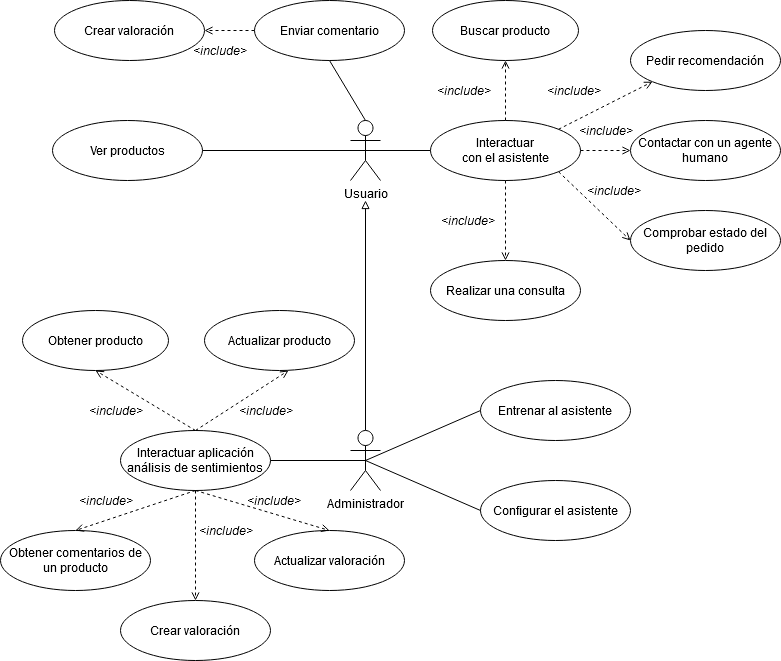
\includegraphics[width =\textwidth]{Figuras/DiagramaCasosUso.png}
	\end{center}
	\caption{\label{fig:casosUso} Diagrama de casos de uso}
\end{figure}

\newpage

\subsection{Descripción de actores del sistema}

A continuación, se describen los actores del sistema (A):

\begin{table}[htbp]
  \centering
    \scalebox{0.85}[0.85] {
    \begin{tabular}{l p{32.145em}}
    \toprule
    \textbf{A001} & \textbf{Usuario} \\
    \midrule
    Requisitos asociados & RF001, RF002, RF003, RF008, RF009, RF010, RF011, RF012, RF013. \\
    Descripción & Formado por todas las personas que accedan a la página web. \\
    Comentarios & Ninguno. \\
    \midrule
    \end{tabular}%
    }
  \label{tab:a003}
\end{table}%

\begin{table}[!htbp]
  \centering
  \scalebox{0.85}[0.85] {
    \begin{tabular}{l p{32.145em}}
    \toprule
    \textbf{A002} & \textbf{Administrador} \\
    \midrule
    Requisitos asociados & RF001, RF002, RF003, RF004, RF005, RF006, RF007, RF008, RF009, RF010, RF011, RF012, RF013, RF014, RF015. \\
    Descripción & Formado por las responsables del sistema. \\
    Comentarios & Ninguno. \\
    \midrule
    \end{tabular}%
  }
  \label{tab:a002}
\end{table}%

\subsection{Descripción de casos de uso del sistema}

Se procede a especificar los casos de uso del sistema que han sido identificados:

\begin{table}[htbp]
  \centering
  \scalebox{0.85}[0.85] {
    \begin{tabular}{l p{32.145em}}
    \toprule
    \textbf{RF0001} & \textbf{Ver productos} \\
    \midrule
    Requisitos asociados & Ninguno. \\
    Descripción & Un usuario (A001) podrá acceder al catálogo completo de productos disponibles en la tienda. \\
    Precondición & Ninguna. \\
    Postcondición & Ninguna.\\
    Comentarios & Ninguno. \\
    \midrule
    \end{tabular}%
  }
  \label{tab:rf001}
\end{table}%

\begin{table}[!htbp]
  \centering
    \scalebox{0.85}[0.85] {
    \begin{tabular}{l p{32.145em}}
    \toprule
    \textbf{RF0002} & \textbf{Enviar comentario} \\
    \midrule
    Requisitos asociados & RNF002. \\
    Descripción & Un usuario (A001) podrá publicar su opinión sobre un producto. \\
    Precondición & Ninguna. \\
    Postcondición & El sistema mostrará el comentario introducido.\\
    Comentarios & Si el usuario no ha iniciado sesión, el comentario será publicado como anónimo. \\
    \midrule
    \end{tabular}%
  }
  \label{tab:rf002}
\end{table}%

\begin{table}[htbp]
  \centering
  \scalebox{0.85}[0.85] {
    \begin{tabular}{l p{32.145em}}
    \toprule
    \textbf{RF0003} & \textbf{Crear valoración} \\
    \midrule
    Requisitos asociados & RNF002, RNF003, RNF004. \\
    Descripción & De forma general, sólo se creará una valoración cuando un usuario (A001) introduzca un comentario. Aunque el administrador (A002) podrá realizar una petición directa al servicio de la API. \\
    Precondición & Enviar un comentario o realizar una llamada a la API incluyendo un token de autenticación. \\
    Postcondición & Se actualizará el valor de puntuación y magnitud del comentario. \\
    Comentarios & La puntuación se muestra gráficamente en la tienda junto a la opinión evaluada. \\
    \midrule
    \end{tabular}%
  }
  \label{tab:rf003}
\end{table}%

\begin{table}[htbp]
  \centering
  \scalebox{0.85}[0.85] {
    \begin{tabular}{l p{32.145em}}
    \toprule
    \textbf{RF004} & \textbf{Obtener producto} \\
    \midrule
    Requisitos asociados & RNF004. \\
    Descripción & Un administador (A002) solicita información sobre un producto. \\
    Precondición & Incluir un token de autenticación y un nombre de producto válidos. \\
    Postcondición & Se ofrecerá el nombre, ID y puntuación media del producto. \\
    Comentarios & La puntuación es la media de los comentarios del producto. \\
    \midrule
    \end{tabular}%
  }
  \label{tab:rf004}
\end{table}%

\begin{table}[htbp]
  \centering
  \scalebox{0.85}[0.85] {
    \begin{tabular}{l p{32.145em}}
    \toprule
    \textbf{RF005} & \textbf{Actualizar producto} \\
    \midrule
    Requisitos asociados & RNF004. \\
    Descripción & Un administador (A002) solicita actualizar la puntuación de un producto. \\
    Precondición & Incluir un token de autenticación y un nombre de producto válidos. \\
    Postcondición & Se ofrecerá el nombre, ID y puntuación media del producto. \\
    Comentarios & La puntuación es la media de los comentarios del producto. \\
    \midrule
    \end{tabular}%
  }
  \label{tab:rf005}
\end{table}%


\begin{table}[htbp]
  \centering
  \scalebox{0.85}[0.85] {
    \begin{tabular}{l p{32.145em}}
    \toprule
    \textbf{RF006} & \textbf{Obtener comentarios de un producto} \\
    \midrule
    Requisitos asociados & RNF004. \\
    Descripción & Un administador (A002) solicita los comentarios de un producto. \\
    Precondición & Incluir un token de autenticación y un ID de producto válidos. \\
    Postcondición & Se listarán todos los comentarios pertenecientes a dicho producto. \\
    Comentarios & Ninguno. \\
    \midrule
    \end{tabular}%
  }
  \label{tab:rf006}
\end{table}%

\newpage

\begin{table}[htbp]
  \centering
  \scalebox{0.85}[0.85] {
    \begin{tabular}{l p{32.145em}}
    \toprule
    \textbf{RF007} & \textbf{Actualizar valoración} \\
    \midrule
    Requisitos asociados & RNF002, RNF003, RNF004. \\
    Descripción & Un administador (A002) solicita actualizar la valoración de un comentario. \\
    Precondición & Incluir un token de autenticación y un ID de comentario válidos. \\
    Postcondición & Se ofrecerá el ID, autor, contenido, puntuación y magnitud del comentario. \\
    Comentarios & Ninguno. \\
    \midrule
    \end{tabular}%
 }
  \label{tab:rf007}
\end{table}%

\begin{table}[!htbp]
  \centering
  \scalebox{0.85}[0.85] {
    \begin{tabular}{l p{32.145em}}
    \toprule
    \textbf{RF008} & \textbf{Interactuar con el chatbot} \\
    \midrule
    Requisitos asociados & RNF001. \\
    Descripción & Un usuario (A001) podrá entablar una conversación con el chatbot. \\
    Precondición & Ninguna. \\
    Postcondición & El agente presentará mediante un menú las acciones que puede realizar.\\
    Comentarios & Será accesible desde cualquier parte de la página web. \\
    \midrule
    \end{tabular}%
 }
  \label{tab:rf008}
\end{table}%

\begin{table}[htbp]
  \centering
  \scalebox{0.85}[0.85] {
    \begin{tabular}{l p{32.145em}}
    \toprule
    \textbf{RF009} & \textbf{Buscar producto} \\
    \midrule
    Requisitos asociados & RNF001. \\
    Descripción & Un usuario (A001) podrá solicitar la ayuda del chatbot para buscar un producto. \\
    Precondición & Seleccionar esta acción. \\
    Postcondición & El asistente preguntará al usuario acerca de la categoría y la marca del producto, ofreciendo un enlace a una selección de productos en función de las decisiones del usuario \\
    Comentarios & Ninguno. \\
    \midrule
    \end{tabular}%
  }
  \label{tab:rf009}
\end{table}%

\begin{table}[!htbp]
  \centering
  \scalebox{0.85}[0.85] {
    \begin{tabular}{l p{32.145em}}
    \toprule
    \textbf{RF010} & \textbf{Pedir recomendación} \\
    \midrule
    Requisitos asociados & RNF001. \\
    Descripción & Un usuario (A001) podrá solicitar una recomendación al chatbot.  \\
    Precondición &  Seleccionar esta acción.\\
    Postcondición & El asistente preguntará al usuario acerca de la categoría y la marca del producto, ofreciendo un enlace a una selección de productos en función de las decisiones del usuario. \\
    Comentarios & El chatbot recomendará el producto mejor valorado. \\
    \midrule
    \end{tabular}%
  }
  \label{tab:rf010}
\end{table}%

\begin{table}[htbp]
  \centering
  \scalebox{0.85}[0.85] {
    \begin{tabular}{l p{32.145em}}
    \toprule
    \textbf{RF011} & \textbf{Contactar con un agente humano} \\
    \midrule
    Requisitos asociados & RNF001. \\
    Descripción & Un usuario (A001) podrá solicitar contactar con un agente humano. \\
    Precondición & Seleccionar esta acción. \\
    Postcondición & El chatbot ofrecerá un enlace al formulario de contacto. \\
    Comentarios & Ninguno. \\
    \midrule
    \end{tabular}%
  }
  \label{tab:rf011}
\end{table}%

\begin{table}[htbp]
  \centering
  \scalebox{0.85}[0.85] {
    \begin{tabular}{l p{32.145em}}
    \toprule
    \textbf{RF012} & \textbf{Comprobar estado del pedido} \\
    \midrule
    Requisitos asociados & RNF001. \\
    Descripción & Un usuario (A001) podrá solicitar información sobre el estado de su pedido. \\
    Precondición & Seleccionar esta acción e introducir un número de pedido válido. \\
    Postcondición & El chatbot informará al usuario que recibirá un correo con la información de dicho pedido. \\
    Comentarios & Un número de pedido válido se compone de 5 cifras. \\
    \midrule
    \end{tabular}%
  }
  \label{tab:rf012}
\end{table}%

\begin{table}[htbp]
  \centering
  \scalebox{0.85}[0.85] {
    \begin{tabular}{l p{32.145em}}
    \toprule
    \textbf{RF013} & \textbf{Realizar una consulta} \\
    \midrule
    Requisitos asociados & RNF001. \\
    Descripción & Un usuario (A001) podrá plantear preguntas sobre su cuenta, pedido, formas de pago, envios, etc. \\
    Precondición & Seleccionar esta acción y formular la pregunta. \\
    Postcondición & El chatbot responderá de manera breve y adjuntará un enlace al centro de atención al cliente. \\
    Comentarios & Ninguno. \\
    \midrule
    \end{tabular}%
  }
  \label{tab:rf013}
\end{table}%

\begin{table}[htbp]
  \centering
  \scalebox{0.85}[0.85] {
    \begin{tabular}{l p{32.145em}}
    \toprule
    \textbf{RF014} & \textbf{Entrenar el asistente} \\
    \midrule
    Requisitos asociados & RNF001. \\
    Descripción &  El administrador (A002) puede añadir nuevos registros para aumentar el conocimiento del chatbot\\
    Precondición & Acceder al servicio de Dialogflow. \\
    Postcondición & Ninguna. \\
    Comentarios & Ninguno. \\
    \midrule
    \end{tabular}%
  }
  \label{tab:rf014}
\end{table}%


\begin{table}[htbp]
  \centering
  \scalebox{0.85}[0.85] {
    \begin{tabular}{l p{32.145em}}
    \toprule
    \textbf{RF015} & \textbf{Configurar el asistente} \\
    \midrule
    Requisitos asociados & RNF001. \\
    Descripción & El administrador (A002) pude modificar las funcionalidades del chatbot. \\
    Precondición & Acceder al servicio de Dialogflow. \\
    Postcondición & Ninguno. \\
    Comentarios & Ninguna. \\
    \midrule
    \end{tabular}%
  }
  \label{tab:rf015}
\end{table}%

\newpage
\section{Requisitos funcionales}

Los requisitos funcionales del sistema coinciden con los casos de uso expuestos en la sección anterior. Son los siguientes:

\begin{itemize}
    \item \textbf{RF001} Ver productos
    \item \textbf{RF002} Enviar comentario
    \item \textbf{RF003} Crear valoración
    \item \textbf{RF004} Obtener producto
    \item \textbf{RF005} Actualizar producto
    \item \textbf{RF006} Obtener comentarios de un producto
    \item \textbf{RF007} Actualizar valoración
    \item \textbf{RF008} Interactuar con el chatbot
    \item \textbf{RF009} Buscar producto
    \item \textbf{RF010} Pedir recomendación
    \item \textbf{RF011} Contactar con un agente humano
    \item \textbf{RF012} Comprobar estado del pedido
    \item \textbf{RF013} Realizar una consulta
    \item \textbf{RF014} Entrenar al asistente
    \item \textbf{RF015} Configurar el asistente
    
\end{itemize}

\section{Requisitos no funcionales}

Por un lado los requisitos no funcionales relacionados con la disponibilidad temporal del sitio web están fijados por los SLAs (Service Level Agreement) que establecen los servicios de Google Cloud y son:
\begin{itemize}
    \item El servicio Cloud Run debe estar disponible el 99.95\% del tiempo.
    \item La base de datos en Cloud SQL debe estar disponible el 99.95\% del tiempo.
    \item El servicio de Dialogflow debe permanecer activo más del 99.9\% del tiempo.
    \item El servicio de Natural Language debe estar también disponible más del 99.9\% del tiempo.
\end{itemize}

\newpage

El resto de requisitos no funcionales son:

\begin{table}[htbp]
  \centering
  \scalebox{0.85}[0.85] {
    \begin{tabular}{l p{32.145em}}
    \toprule
    \textbf{RNF001} & \textbf{Lenguaje soportado por el chatbot} \\
    \midrule
    Descripción & El lenguaje principal del bot conversacional será el español. \\
    Comentarios & Puede configurarse para soportar otros lenguajes. \\
    \midrule
    \end{tabular}%
  }
  \label{tab:rnf001}
\end{table}%

\begin{table}[htbp]
  \centering
  \scalebox{0.85}[0.85] {
    \begin{tabular}{l p{32.145em}}
    \toprule
    \textbf{RNF002} & \textbf{Lenguajes utilizados en los comentarios} \\
    \midrule
    Descripción & Los comentarios publicados por los clientes pueden ser en inglés, español, francés, alemán, italiano, japonés, coreano, portugués (brasileño y continental) y chino (simplificado y tradicional). \\
    Comentarios & Son los lenguajes soportados por Google NLP. \\
    \midrule
    \end{tabular}%
  }
  \label{tab:rnf002}
\end{table}%

\begin{table}[!htbp]
  \centering
  \scalebox{0.85}[0.85] {
    \begin{tabular}{l p{32.145em}}
    \toprule
    \textbf{RNF003} & \textbf{Sistema de puntuación} \\
    \midrule
    Descripción & La puntuación de los comentarios se mostrará en forma de estrellas. \\
    Comentarios & Ninguna. \\
    \midrule
    \end{tabular}%
  }
  \label{tab:rnf003}
\end{table}%

\begin{table}[!htbp]
  \centering
  \scalebox{0.85}[0.85] {
    \begin{tabular}{l p{32.145em}}
    \toprule
    \textbf{RNF004} & \textbf{Seguimiento de errores} \\
    \midrule
    Descripción & La aplicación de análisis de sentimientos deberá almacenar logs de los errores. \\
    Comentarios & El almacenamiento se realizará en la nube utilizando Cloud Logging. \\
    \midrule
    \end{tabular}%
  }
  \label{tab:rnf004}
\end{table}%

\section{Análisis económico}

\subsection{Tarifas de los servicios de Google Cloud}

\subsubsection{Google Natural Language Processing}

El precio de este servicio se calcula mensualmente según la funcionalidad utilizada y el número de unidades evaluadas. Cada petición realizada a la API supone una unidad; si contiene más de 1000 caracteres se cuenta una unidad por cada 1000 caracteres. Por ejemplo, si se envían tres peticiones que contienen 300, 1725 y 850 caracteres respectivamente, se llevará a cabo el cobro por 4 unidades.

A continuación, se muestran en una tabla los precios establecidos por Google por cada 1000 unidades según el total de unidades evaluadas a lo largo de un mes:

\begin{table} [htbp]
	\centering
    \scalebox{0.75}[0.75] {
	\begin{tabular}{l c c c c}
		\textbf{Función} & \textbf{0-5000} & \textbf{5001-1.000.000} & \textbf{1.000.001-5.000.000} & \textbf{5.000.000-20.000.000} \\ \hline
         Análisis de entidades & Gratis & 1 USD & 0,50 USD & 0,25 USD \\
         Análisis de opinión & Gratis & 1 USD & 0,50 USD & 0,25 USD \\
         Análisis sintáctico & Gratis & 0,50 USD & 0,25 USD & 0,125 USD \\
         Análisis de opinión de entidades & Gratis & 2 USD & 1 USD & 0,50 USD \\
	\end{tabular}}
	\centering
	\caption{\label{tab:costeNLP}Precios mensuales Cloud Natural Language. Fuente: Google Cloud.}
\end{table}

\newpage

\subsubsection{Cloud Run}

Dada una instancia de un contenedor, el tiempo de facturación comienza cuando la instancia está procesando al menos una petición. Si dicha instancia recibe varias peticiones al mismo tiempo, la facturación comienza cuando llega la primera petición y termina cuando se resuelve la última petición. En el siguiente diagrama se puede observar esta situación:

\begin{figure}[ht]
	\begin{center}
		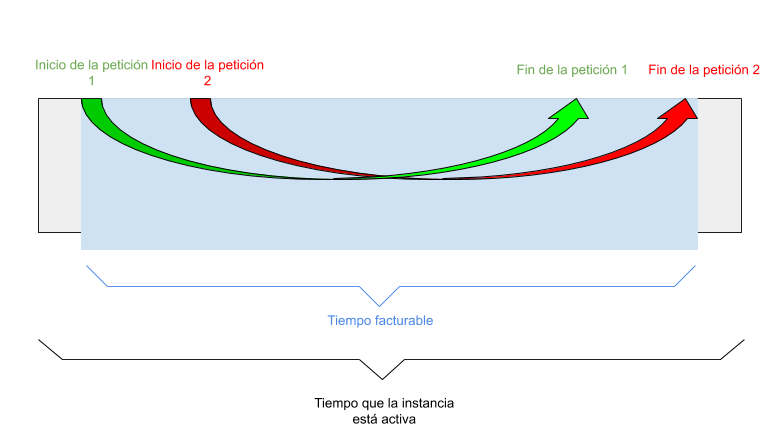
\includegraphics[width = 0.95\textwidth]{Figuras/FacturacionCloudRun.png}
	\end{center}
	\caption{\label{fig:facturacionCloudRun} Tiempo facturable Cloud Run. Fuente: Google Cloud.}
\end{figure}


A continuación, se exponen en una tabla los precios establecidos para el servicio utilizando como unidad el GiB/s, es decir ejecutar una instancia de 1 GiB durante un segundo. La unidad vCPU indica lo mismo, uso por segundo de vCPU.

\begin{table} [htbp]
	\centering
	 \scalebox{0.75}[0.75] {
	\begin{tabular}{l l l l}
		\textbf{CPU} & \textbf{Memoria} & \textbf{Solicitudes} & \textbf{Redes} \\ 
		\hline
		180.000 vCPU/s gratuitas &
		360.000 GiB gratuitos &
		2 millones gratuitas &
		1 GiB gratuito en Norteamérica \\
		
		0.000024 USD por vCPU/s &
		0.00000250 USD GiB/s &
		0,40 USD por millón &
		Depende de la geolocalización \\

	\end{tabular}}
	\centering
	\caption{\label{tab:costeCloudRun}Precios por uso de Cloud Run. Fuente: Google Cloud.}
\end{table}

Sólo se cobrará por el uso de Cloud Run cuando se supere la cantidad gratuita. Esta cuota es compartida por todos los proyectos pertenecientes a la misma cuenta de facturación y se renueva mensualmente.

\subsubsection{Cloud SQL}

El coste de este servicio depende principalmente del tipo de instancia utilizada y la región en la que se sitúe. Este cargo se calcula por minuto de ejecución de la instancia. Por ejemplo, el coste por mes de una instancia \textit{db-n1-standard-2} sería:

\begin{table} [htbp]
	\centering
	\scalebox{0.85}[0.85] {
	\begin{tabular}{c c c c c c c}
		\textbf{CPU} & \textbf{RAM} & \textbf{Almacenamiento} & \textbf{Conexiones} & 
		\textbf{Precio} & \textbf{Precio de alta disponibilidad}	\\ 
		\hline
         2 & 7,5 & 30.720 GB & 4000 & 49,31 USD & 98,62 USD\\
	\end{tabular}}
	\centering
	\caption{\label{tab:costeMySQL}Precios mensuales de instancias MySQL. Fuente: Google Cloud.}
\end{table}

Otras opciones de configuración como la capacidad de almacenamiento, el tipo (SSD o HDD) y el número de copias de seguridad también influyen en el precio final:

\begin{itemize}
    \item SSD: 0,170 USD por GB/Mes
    \item HDD: 0,090 USD por GB/Mes
    \item Copias de seguridad: 0,080 USD por GB/Mes
\end{itemize}

Además, pueden cobrarse cargos adicionales según el destino del tráfico a la salida de Cloud SQL: 

\begin{itemize}
    \item Instancias de Compute Engine y réplicas interregionales de Cloud SQL: si es en la misma región, gratis; 0,12 USD/GB entre regiones dentro y fuera de Norteamérica.
    \item Productos de Google (sin contar Compute Engine): si es intracontinental, gratis. En caso contrario 0,12 USD/GB.
    \item Salida a Internet a través de Cloud Interconnect: 0,05 USD/GB.
    \item Salida a Internet sin Cloud Interconnect: 0,19 USD/GB.
\end{itemize}

Por último, aspectos como el tiempo que el usuario se comprometa a hacer uso de este servicio también tienen impacto sobre el coste total. 

Con tantos factores influyendo sobre el coste total se puede comprobar que es difícil conocer exactamente la cuantía que deberá afrontar la empresa.

\subsubsection{Container Registry}

Para almacenar las imágenes en Container Registry se crea un segmento de almacenamiento de Cloud Storage, que de forma predeterminada es de tipo Standard. El coste para este tipo de segmentos es de 0,026 USD por GB al mes. 

\newpage

En la siguiente tabla aparecen reflejados los precios por GB al mes para cada tipo de segmento de Cloud Storage:

\begin{table} [htbp]
	\centering
	\begin{tabular}{l c c c c}
		\textbf{Standard} & \textbf{Nearline} & \textbf{Coldline} & \textbf{Archive} \\ \hline
         0.026 USD & 0.010 USD & 1 0.007 USD & 0.004 USD \\
	\end{tabular}
	\centering
	\caption{\label{tab:costeCloudStorage}Precios mensuales Cloud Storage. Fuente: Google Cloud.}
\end{table}

Si se desea realizar un análisis de vulnerabilidades sobre las imágenes subidas, supone un coste de 0,26 USD por imagen. Sin embargo, sólo se cobrará la primera vez que se analice cada imagen, es decir, no se cobran análisis posteriores sobre la misma imagen.

\subsubsection{Cloud Logging}

Los primeros 50 GiB usados por proyecto serán gratuitos, a partir de aquí se aplicará una tarifa de 0,50 USD por cada GiB adicional.

\subsubsection{Dialogflow}

Actualmente DialogFlow cuenta con tres planes diferentes de pago, como en este proyecto solo se hace uso de peticiones en forma de texto, se van a comparar estos planes en función de sus cuotas para texto.
\begin{itemize}
    \item \textbf{Edición estándar}. Es gratuito, pero se encuentra limitado por límite de peticiones que se pueden realizar; permite hasta un máximo de 180 solicitudes por minuto.
    \item \textbf{Edición empresarial}. Ofrece cuotas de uso más elevadas y además asistencia técnica por parte de Google Cloud. Dentro de esta edición se distinguen dos formatos:
    \begin{itemize}
        \item Essentials. Permite hasta 600 peticiones por minuto con un precio de 0,002 USD por solicitud.
        \item Plus. Se trata de la versión más avanzada, contiene todas las funcionalidades de Essentials y ofrece más opciones respecto a los conectores de conocimiento. Permite hasta 600 peticiones por minuto con un precio de 0,004 USD por solicitud.
    \end{itemize}
\end{itemize}


\subsection{Presupuesto de realización del proyecto}

Se procede a detallar el coste económico que ha supuesto la realización de este proyecto, para ello se tomará como referencia la estimación de horas expuesta en el apartado Fases de desarrollo. Conviene indicar que no sólo se tiene en cuenta el tiempo dedicado, también se consideran los costes asociados a los recursos utilizados durante el desarrollo.

\subsubsection{Costes directos}

Se entiende por costes directos aquellos que están directamente relacionados con el desarrollo del producto y la determinación el precio de venta. A continuación se exponen los costes directos a los que se ha tenido que hacer frente:

\begin{itemize}
    \item \textbf{Capital Humano}. Habría que establecer dos precios distintos para cada miembro debido a las diferencias de experiencia y conocimientos entre el autor y el alumno. Sin embargo, sólo se tendrá como referencia el trabajo realizado por el alumno para el cómputo del coste. Estableciendo un precio de 18€/hora, el coste total sería de:
    \begin{equation}
        300h \times 18\textup{€}/h = 5400\textup{€}
    \end{equation}
    \item \textbf{Hardware}. El único equipamiento hardware que se ha necesitado para el desarrollo del proyecto ha sido el de un ordenador portátil. En concreto, se trata de un ordenador MSI con 8 GB de memoria RAM y un procesador i7. En el momento de su adquisición supuso un coste de 800€.
    \item \textbf{Software}. Todo el software utilizado es gratuito, sin embargo cabe destacar que los servicios cloud utilizados no han supuesto ningún coste adicional porque se han utilizado sus planes más básicos que suelen ser gratuitos. Una vez que el sistema se encuentre en funcionamiento, quizás el plan más básico no sea suficiente y haya que aumentar las prestaciones ocasionando un incremento de los gastos.
\end{itemize}

\subsubsection{Costes totales}

Para obtener el coste total del proyecto, se añaden a los costes directos un 20\% de los mismos en concepto de costes indirectos.

\begin{table} [htbp]
	\centering
	\begin{tabular}{l c c}
		\textbf{Tipo de coste} & \textbf{Importe}\\ \hline
         Capital humano & 5400€ \\
         Hardware & 800€ \\
         Software & 0€ \\
         Costes indirectos & 1240€ \\
         \hline
         Coste total & 7440€ \\ 
	\end{tabular}
	\centering
	\caption{\label{tab:presupuesto}Presupuesto}
\end{table}

Los costes indirectos reflejados en el cálculo del presupuesto son aquellos en los que incurre la empresa pero que no puede imputar directamente al proceso de producción. Aquí se incluyen los gastos ocasionados por la factura de luz e internet, el desplazamiento para acudir a tutorías con el tutor, etc.
\chapter{Tecnologías y Herramientas} 
\label{sec:tecnologia}

\section{Postman}

Es una herramienta muy útil, orientada a los desarrolladores, que permite realizar peticiones de una forma sencilla e intuitiva a cualquier API. En este proyecto se ha usado Postman para comprobar el correcto funcionamiento de la API desarrollada.

\section{Git}

Es un programa para el control de versiones que permite: mantener un historial de todos los cambios realizados en el código de un proyecto y coordinar el trabajo de un equipo sobre archivos compartidos.
En este proyecto se ha utilizado Git para subir los cambios a un repositorio externo; sin embargo, no se han tenido que utilizar distintas ramas de desarrollo porque todo el trabajo ha sido individual.

\section{Github}

Es un sitio web destinado al alojamiento de código que utiliza Git. Se caracteriza por sus funciones colaborativas permitiendo que cualquier persona pueda visualizar y descargar el código fuente, sugerir cambios y ayudar a mejorar el proyecto. Si un usuario desea restringir el acceso a su repositorio pueden crearse proyectos privados.

\section{Trello}

Es una herramienta creada para facilitar la gestión de proyectos, que cuenta con una interfaz web y un cliente para iOS y Android. Permite crear y organizar tareas en forma de "tarjetas" y organizarlas en diferentes bloques. Cada uno de estos bloques se identifica con una etapa diferente del flujo de trabajo, de modo que durante el desarrollo las tarjetas se van moviendo de un bloque a otro para identificar el estado actual de la tarea. 


\section{Visual Studio Code}

Se encuentra a medio camino entre un editor de texto y un IDE. Fue desarrollado por Microsoft y es multiplataforma (Windows, Linux y macOS). Gracias al amplio ecosistema de plugins que posee permite trabajar con una gran cantidad de lenguajes de programación (Go, Python, C, C++, etc.). Incluye funcionalidades como la finalización de código inteligente, refactorización de código, soporte de depuración, entre otros.

\section{Xampp}

Es la herramienta más utilizada para la instalación de entornos de desarrollo, consistente en un conjunto de herramientas que se enumeran a continuación:

\begin{itemize}
    \item \textbf{MariaDB}. Es un sistema de gestión de bases de datos creado a partir de MySQL. MariaDB nació como una bifurcación directa de MySQL cuando éste fue adquirido por Oracle para asegurar que se mantuviese como software libre. MariaDB cuenta con todas las funcionalidades de MySQL, aunque añade otras relacionadas con los mecanismos de almacenamiento y la facilidad de uso.  
    \item \textbf{Apache}. Es un servidor web HTTP de código abierto y multiplataforma que destaca por su facilidad de uso y popularidad. Apache implementa el protocolo HTTP/1.1.
    \item \textbf{Perl}. Se trata de un lenguaje de programación inspirado en lenguajes como C, Shell y AWK, entre algunos otros. Fue ampliamente adoptado por su facilidad para el procesamiento de textos, tareas como extraer información y generar informes a partir del contenido de archivos de texto.
    \item \textbf{PHP}. Es el lenguaje más utilizado para el desarrollo web en el lado del servidor. En un principio era conocido como Personal Home Page Tools y se trataba de un CGI capaz de interpretar unos pocos comandos. Durante el paso de los años fue objeto de una serie de mejoras que lo han convertido en lo que hoy conocemos por PHP (PHP: Hypertext Preprocessor).
\end{itemize}

\section{Wordpress}
En primer lugar, es necesario definir el concepto de CMS (Content Management System). Como su propio nombre indica, se trata de una aplicación software o un conjunto de programas relacionados que son usados para la creación y administración de contenido digital. 

Alrededor de un 60\% de las páginas web que podemos encontrar hoy en día hacen uso de un CMS. De entre todas esas páginas, el 64,3\% están construidas con Wordpress \citeW{W3Techs:1}. En la siguiente figura se puede observar la tendencia de uso que han seguido los diferentes CMS a lo largo de los últimos diez años \citeW{W3Techs:2}: 

\begin{figure}[ht]
	\begin{center}
		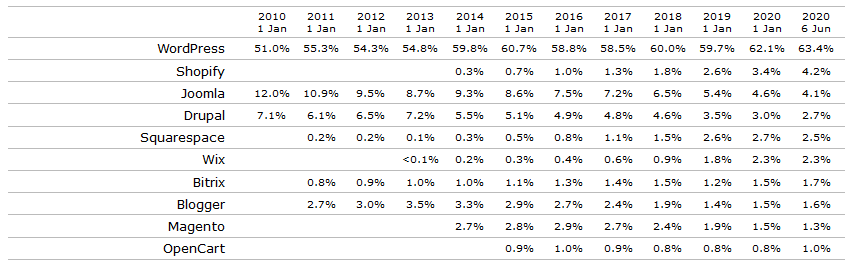
\includegraphics[width = 0.95\textwidth]{Figuras/TendenciaUsoCMS.PNG}
	\end{center}
	\caption{\label{fig:CMS} Tendencia de uso de los CMS. Fuente: W3Techs.}
\end{figure}

Como se puede observar, Wordpress ha sido el líder de los CMS durante diez años seguidos y presenta una diferencia muy notable respecto a su competidor más cercano.

Por ser el más popular cuenta con una gran variedad de plantillas de diseño y plugins que permiten añadir cualquier tipo de funcionalidad que se pueda imaginar. Haciendo uso de uno estos plugins, se puede implementar una tienda virtual de forma sencilla e intuitiva sin requerir de conocimientos técnicos avanzados. Es por esta razón por la que gran parte de las pymes diseñan sus sitios webs utilizando Wordpress.

Al adoptar esta tecnología se pretende demostrar que cualquier empresa dedicada al comercio electrónico puede incorporar herramientas de IA en su tienda en línea.

\newpage

\subsection{WooCommerce}

Se trata de una extensión gratuita para Wordpress que permite transformar una página web en una tienda de comercio electrónico en cuestión de minutos. Aunque la venta de productos es el escenario más obvio para la creación de una tienda, WooCommerce también soporta la creación de webs destinadas a la venta de servicios o suscripciones. 
Es la plataforma de comercio electrónico líder en 2020 con un 28,24\% de cuota de mercado \citeW{statista}:

\begin{figure}[ht]
	\begin{center}
		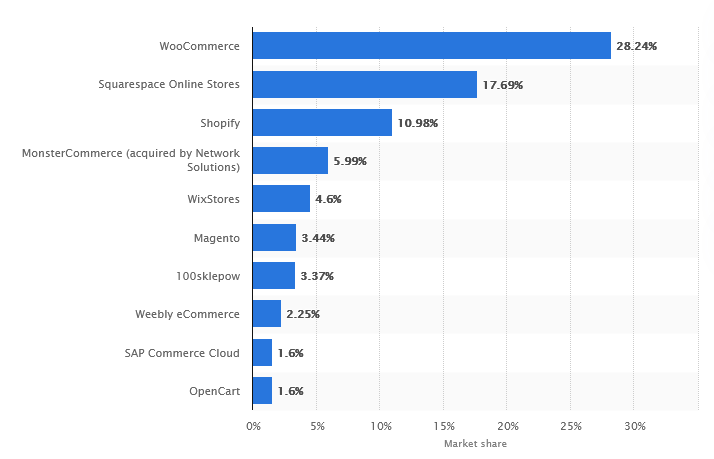
\includegraphics[width = 0.80\textwidth]{Figuras/eCommerceMarketShare.PNG}
	\end{center}
	\caption{\label{fig:WooCommerce} Cuota de mercado de las principales plataformas de comercio electrónico. Fuente: Statista.}
\end{figure}

Existen más de 50.000 plugins de Wordpress específicamente desarrollados para WooCommerce, ofreciendo al usuario la capacidad de personalizar completamente su tienda.

\subsection{MyChatbot}

De manera sencilla, se puede definir un chatbot como un servicio de software que responde automáticamente a las preguntas que se le plantean a través de una interfaz de chat. Su uso en el comercio electrónico permite aportar soluciones a los clientes las 24 horas del día sin necesidad de que participe ningún empleado.

Existen multitud de plugins que permiten incorporar un bot conversacional a Wordpress,  la mayoría de éstos ofrecen un sistema entrenado o cuentan con un constructor para facilitar la tarea a los usuarios. Sin embargo, en este trabajo sólo se pretende conectar Wordpress con un motor conversacional desarrollado en una plataforma externa.

Con este objetivo se ha elegido MyChatbot, una herramienta gratuita que utiliza Dialogflow —plataforma de comprensión del lenguaje natural perteneciente a Google— como motor conversacional. Seguidamente se muestra un ejemplo de este plugin:

\begin{figure}[ht]
    \begin{center}
    	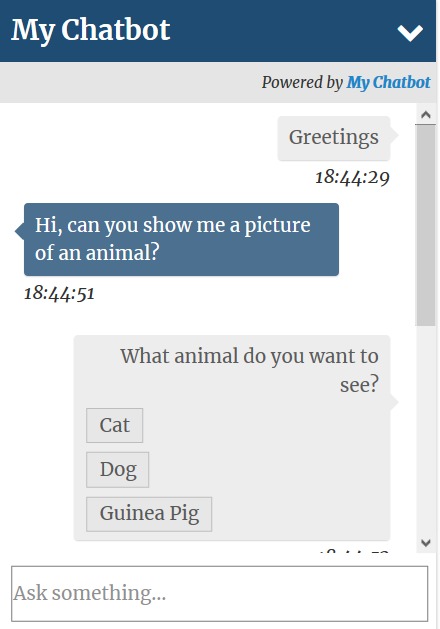
\includegraphics[width = 0.30\textwidth]{Figuras/chatbotExample.PNG}
    \end{center}
    \caption{\label{fig:myChatbot} Ejemplo de MyChatbot en funcionamiento. Fuente: My Chatbot WordPress plugin demo.}
\end{figure}

\subsection{WP-Stateless}
La página web implementada será desplegada haciendo uso de Cloud Run. Esta plataforma ejecuta contenedores sin estado, por tanto, los cambios que se realicen durante la ejecución del contenedor no se guardarán si se reinicia el servicio. No obstante, esta característica no tiene impacto sobre aquella información que se almacena en la base de datos, pero sí afecta a los archivos multimedia, como las imágenes que ilustran un producto.

WP-Stateless es una extensión de Wordpress que almacena todos los archivos que se suben en un segmento de Google Cloud Storage para hacerlos persistentes. En cuanto a su configuración, el proceso es muy sencillo, tan sólo se debe elegir un proyecto existente de Google Cloud y el resto de campos se completará automáticamente.

\newpage

\section{GoLang}

Go es un lenguaje de programación multiplataforma moderno, muy potente y simple. Es una elección excelente para aplicaciones cloud y orientadas a microservicios. Go está ganando popularidad a pasos agigantados y está atrayendo a muchos programadores. Tal es el hecho, que en la encuesta realizada por StackOverflow a 65000 desarrolladores, Go figura como el quinto lenguaje favorito y el tercero más buscado \citeW{StackOverflow}. A continuación, se muestran los resultados de dicha encuesta: 

\begin{figure}[ht]
	\begin{center}
		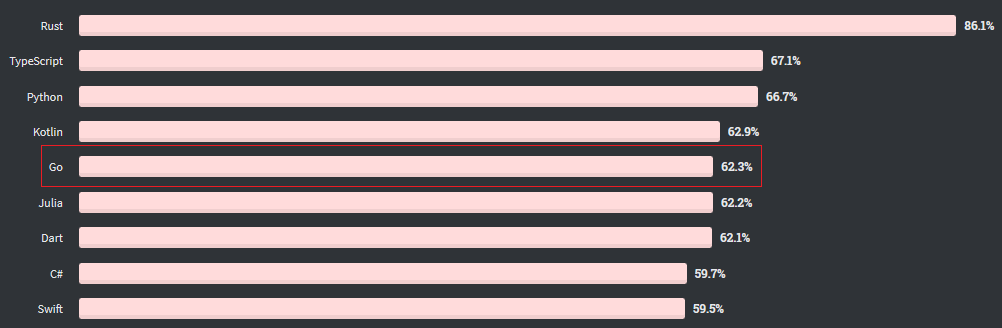
\includegraphics[width = 0.95\textwidth]{Figuras/queridos.png}
	\end{center}
	\caption{\label{fig:Loved} Lenguajes favoritos de los desarrolladores en 2020. Fuente: StackOverflow.}
\end{figure}

\begin{figure}[ht]
	\begin{center}
		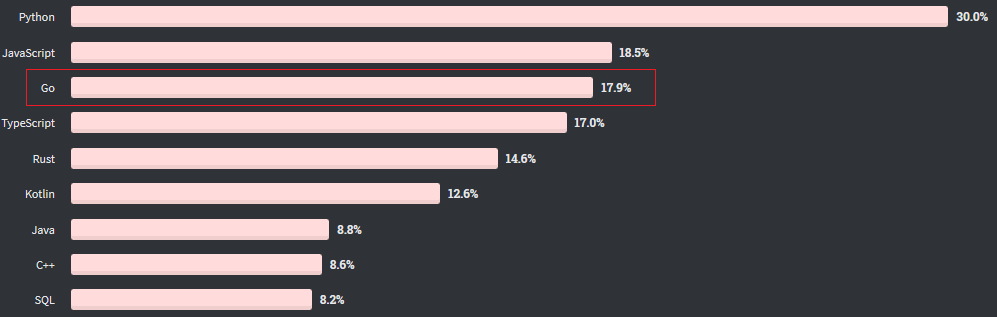
\includegraphics[width = 0.95\textwidth]{Figuras/buscados.png}
	\end{center}
	\caption{\label{fig:Wanted} Lenguajes más buscados por los desarrolladores en 2020. Fuente: StackOverflow.}
\end{figure}

\section{Dockers}

Un contenedor es una unidad de software que empaqueta el código y todas sus dependencias para que la aplicación pueda ejecutarse en cualquier entorno informático asegurando su funcionamiento uniformemente a pesar de las diferencias como, por ejemplo, desarrollo y producción. Una imagen de contenedor es un paquete de software ligero, independiente y ejecutable que incluye todo lo necesario para ejecutar una aplicación: código, herramientas del sistema, librerías y configuraciones.

En el caso de los contenedores Docker, su imagen se convierte en contenedor al ejecutarlo con Docker Engine \citeW{Docker}. 

A menudo, las personas que se inician en esta tecnología tienden a confundirla con la funcionalidad de los contenedores tradicionales de Linux. Si bien es verdad que Docker surgió a partir de la tecnología LXC (Linux containers), actualmente se encuentra muy alejado de su influencia. LXC sólo era un método de virtualización ligera. Sin embargo, Docker va más allá, no sólo provee la capacidad de crear contenedores sino que también ofrece un flujo de trabajo, ayudando a la creación y diseño de contenedores y al envío y creación de versiones de imágenes \citeW{RedHat}.

La tecnología Docker tiene un enfoque granular, en el sentido de que pretende conseguir la separación de las aplicaciones en sus procesos individuales y además ofrece las herramientas para ello. En la siguiente figura se realiza una comparación de ambas tecnologías:

\begin{figure}[ht]
	\begin{center}
		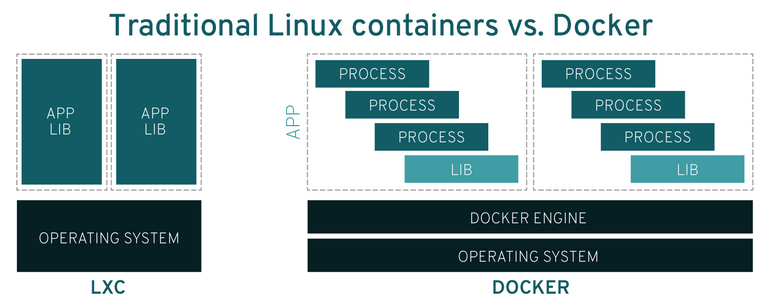
\includegraphics[width = 0.95\textwidth]{Figuras/Docker_LXC.PNG}
	\end{center}
	\caption{\label{fig:Docker_LXC} Comparación de LXC y Docker. Fuente: Red Hat.}
\end{figure}

Docker-Engine esta formado por tres componentes principales:
\begin{itemize}[leftmargin=+.5in]
    \item Un cliente (\textit{docker}), por medio del cual se pueden ejecutar diferentes comandos como \textit{build}, \textit{run}, \textit{rm}, \textit{push}, \textit{pull}, etc. 
    \item Un servidor (\textit{dockerd}), al que también se puede hacer referencia como demonio si se tiene en cuenta la notación de linux.
    \item Una API REST (\textit{docker registry}), que especifica las interfaces que los programas pueden usar para hablar con el servidor o demonio e indicarle qué hacer.
\end{itemize}

\newpage

A continuación, se presenta en una figura los componentes Docker Engine:

\begin{figure}[ht]
	\begin{center}
		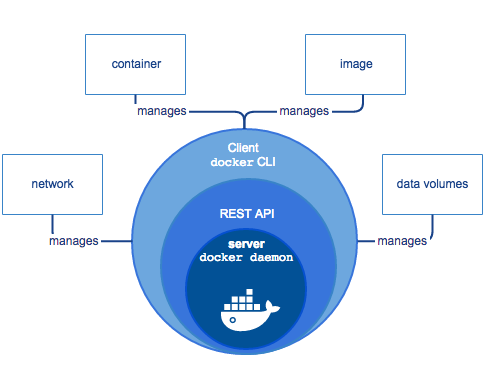
\includegraphics[width = 0.60\textwidth]{Figuras/DockerComponents.png}
	\end{center}
	\caption{\label{fig:DockerComponents} Componentes de Docker Engine. Fuente: docker docs.}
\end{figure}

El cliente Docker interactúa con el demonio Docker, que hace el trabajo pesado de construir, ejecutar y distribuir sus contenedores. El cliente y el demonio pueden ejecutarse en el mismo sistema, o se puede realizar una conexión con un cliente o demonio remotos. Ambos se comunican mediante una API REST, a través de sockets UNIX o una interfaz de red.

\begin{figure}[ht]
	\begin{center}
		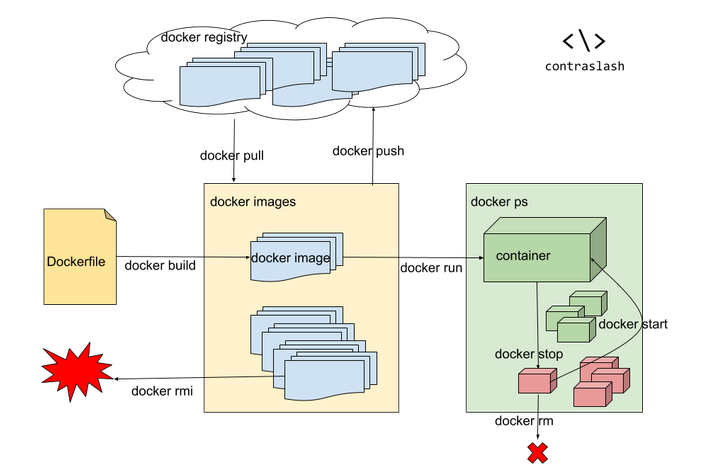
\includegraphics[width = 0.80\textwidth]{Figuras/DockerArchitecture.png}
	\end{center}
	\caption{\label{fig:DockerArchitecture} Arquitectura de Docker. Fuente: contraslash.}
\end{figure}

\section{Servicios cloud de Google}

Para la realización del proyecto se han utilizado diferentes servicios disponibles en Google Cloud. ¿Por qué? Uno de los objetivos del trabajo es desplegar la página web y la aplicación en la nube mediante contenedores. Existen muchas plataformas para realizar este proceso y cada una cuenta con herramientas específicas para ello. Mientras se investigaba sobre todas estas posibilidades, surgió la de utilizar Cloud Run, una plataforma de computación en la nube sin servidores y que fue lanzada al mercado por Google hace tan sólo un año. Este servicio encaja con las necesidades del proyecto, al mismo tiempo que supone un reto, ya que, al ser tan reciente, en la web no se pueden encontrar tantos ejemplos de su uso como de otras opciones. Asimismo, entre los servicios de procesamiento del lenguaje natural, se determinó que uno de los más adecuados era el de Google, debido a que devuelve un valor decimal comprendido entre -1 y 1 que puede ser discretizado para su representación en forma de estrellas. Al optar por dos herramientas de Google Cloud se decidió utilizar esta plataforma para el resto de funcionalidades necesarias.

En esta sección se expondrán cuáles son estos servicios, su rol y la razón de su elección.

\subsection{Google Natural Language Processing}

Esta herramienta permite el análisis de opiniones, el análisis de entidades, el análisis de opiniones sobre entidades, la clasificación de contenido y el análisis sintáctico. El análisis de un texto mediante esta herramienta da como resultado dos valores numéricos:

\begin{itemize}
    \item \textbf{Puntuación}. Número decimal comprendido entre -1,0 (negativo) y 1,0 (positivo). Se corresponde con la tendencia emocional general del texto.
    \item \textbf{Magnitud}. Número decimal comprendido entre 1,0 e $\infty$. Expresa la intensidad de la emoción. Hay que tener en cuenta que para el cálculo de este valor se considera cada expresión de emoción en el texto. Por tanto, los valores de magnitud para textos más largos es probable que sean mayores.
\end{itemize}

Es importante resaltar que este servicio sólo diferencia entre emociones positivas o negativas, pero no es capaz de identificar emociones específicas (furia, sorpresa, tristeza, etc.). 

Para ilustrar el modo de funcionamiento, se procede a analizar la siguiente opinión de un usuario sobre el libro \textit{El lobo estepario} de Herman Hesse en Amazon: “A good read. Smart. But moody and not too readable. But I still remember the story, so it has influence on you.”

\newpage

La salida obtenida al hacer una petición a Google NLP es:

\begin{lstlisting}[caption=Ejemplo de respuesta API NLP ]
"documentSentiment": {
    "magnitude": 2.0,
    "score": 0.4
  },
language": "en",
  "sentences": [
    {...}
  ]
}
\end{lstlisting}

Ofrece una puntuación de 0,4  y magnitud de 2,0 para la opinión de forma general y continúa desgranando los valores para cada una de las frases que la forman. Se puede observar que existe una fuerte intensidad de la emoción, debido a que se alcanza un valor de 2 en un texto formado por dos líneas. A su vez, la puntuación indica que se trata de una opinión positiva, aunque no demasiado.

Si la opinión tiene una puntuación cercana a cero puede deberse a que la intensidad de la emoción es baja o a que presenta emociones mixtas. Por ello, antes de clasificar dicha opinión es necesario eliminar la ambigüedad atendiendo a la magnitud, ya que las opiniones que sean verdaderamente neutrales tendrán un valor de magnitud bajo, mientras que las opiniones con emociones mixtas tendrán un valor alto.

Este servicio presenta una ventaja frente a sus principales competidores porque además de ofrecer una puntuación que oscila en un intervalo, también permite eliminar ambigüedades con otro parámetro de la respuesta.

\subsection{Cloud Run}

Realizar el despliegue de una página web puede llegar a convertirse en una tarea tediosa si se tiene en cuenta la sobrecarga de trabajo que conlleva la creación y administración de clústers, servicios, grupos de contenedores, máquinas virtuales, etc. Esta situación es aceptable si se está tratando con grandes aplicaciones formadas por varios niveles, pero si sólo se desea desplegar y hacer visible un sitio web, es una carga demasiado grande.

Cloud Run permite administrar y desplegar una página web haciendo que el usuario se desentienda de cualquier aspecto relacionado con de la infraestructura y disponibilidad. Se trata de una plataforma que ejecuta contenedores sin estado, esto quiere decir que cualquier cambio que se introduzca en la página web o aplicación durante su ejecución no será persistente. Para afrontar esta situación se pueden tomar dos decisiones, realizar los cambios en local y subir nuevas revisiones o añadir volúmenes al contenedor. 

Cada implementación de un nuevo servicio en Cloud Run crea una revisión. Dicha revisión está compuesta por una imagen de contenedor, la configuración del entorno, las variables de entorno, los límites de memoria y el valor de simultaneidad. Las revisiones son inmutables, es decir, una vez creadas no se podrán modificar. Si se añade una nueva imagen a ese mismo servicio, se crea una nueva revisión. Cuando se modifican los límites de memoria, se crea otra nueva revisión, etc.

Las revisiones que se encuentren recibiendo peticiones escalan automáticamente a la cantidad de contenedores necesarios para hacerse cargo de todas las solicitudes. Además, cuando la revisión no esté recibiendo ninguna petición escalará el número de contenedores a cero. La cantidad máxima de solicitudes que se pueden enviar en paralelo a una instancia de contenedor se puede configurar mediante el valor de simultaneidad \citeW{CloudRun}. 

\subsection{Cloud SQL}
Para su funcionamiento, Wordpress necesita una base de datos MySQL donde almacenar toda la información de la página web, la configuración de los plugins y de los temas.

CloudSQL es un servicio de bases de datos totalmente administrado que es compatible con MySQL, PostgreSQL y SQL Server. En general, las funciones de MySQL que proporciona una instancia de Cloud SQL son las mismas que las que proporciona una instancia de MySQL alojada localmente \citeW{CloudSQL}. 

A la hora de crear la instancia se ofrecen distintas opciones de configuración al usuario:

\begin{itemize}
    \item \textbf{Tipo de almacenamiento}
    \begin{itemize}
        \item SSD. Ofrece un número de consultas por segundo y rendimiento de datos más altos.
        \item HDD. Tiene un rendimiento más bajo comparado con el SSD. Esta opción es la más económica.
    \end{itemize}
    \item \textbf{Capacidad de almacenamiento}
    \newline
    El rendimiento y la capacidad de la instancia son proporcionales. También se puede activar la opción "Habilitar los aumentos automáticos de almacenamiento" permitiendo así que el espacio de almacenamiento aumente cada vez que se esté cerca de alcanzar la capacidad establecida.
    \item \textbf{Copias de seguridad}
    \newline
    Realizar de forma automática las copias de seguridad en el horario seleccionado.
    \item \textbf{Disponibilidad}
     \begin{itemize}
        \item Zona única. En caso de que se produzca una interrupción no se activa la conmutación por error. Esta opción es poco recomendable para instancias de producción.
        \item Alta disponibilidad(regional). Activa la conmutación por error automática hacia otra zona dentro de la región que ha sido seleccionada. Esta opción es más costosa.
    \end{itemize}
    \item \textbf{Mantenimiento}
    \newline
    Permite seleccionar el período de tiempo para llevar a cabo este proceso, ya que durante el mantenimiento la instancia se reinicia, de modo que el servicio se ve interrumpido brevemente.
\end{itemize}

Para la realización de este proyecto se ha hecho uso de una instancia de tipo \textit{db-f1-micro}, que es la configuración más básica permitida y sólo está recomendada para entornos de desarrollo y prueba.

\subsection{Container Registry}

Se trata de un registro privado de imágenes de contenedor que se ejecuta en Google Cloud. Será aquí donde se almacenen las imágenes de contenedor utilizadas en el proyecto. 

Dentro del registro se pueden almacenar multitud de imágenes y cada una de ellas puede constar de varias versiones. Es posible identificar una versión específica de una imagen dentro de un registro haciendo uso de etiquetas (exclusivas a nivel de registro) \citeW{Registry}. 

Cloud Run puede extraer imágenes de Container Registry para ejecutar un servicio y, aunque no sea este el caso, Container Registry también puede integrarse con servicios externos, como por ejemplo, Kubernetes.

\subsection{Cloud Logging}

Es una herramienta de Google Cloud que permite almacenar, buscar, analizar y monitorizar eventos y datos de registros, así como crear registros personalizados haciendo uso de su API. Cuenta con un visor que permite seleccionar entradas de registro filtrando por diferentes opciones, como un periodo específico, nivel de gravedad, origen, etc. En la siguiente figura se muestra el aspecto del visor de registros:

\begin{figure}[ht]
	\begin{center}
		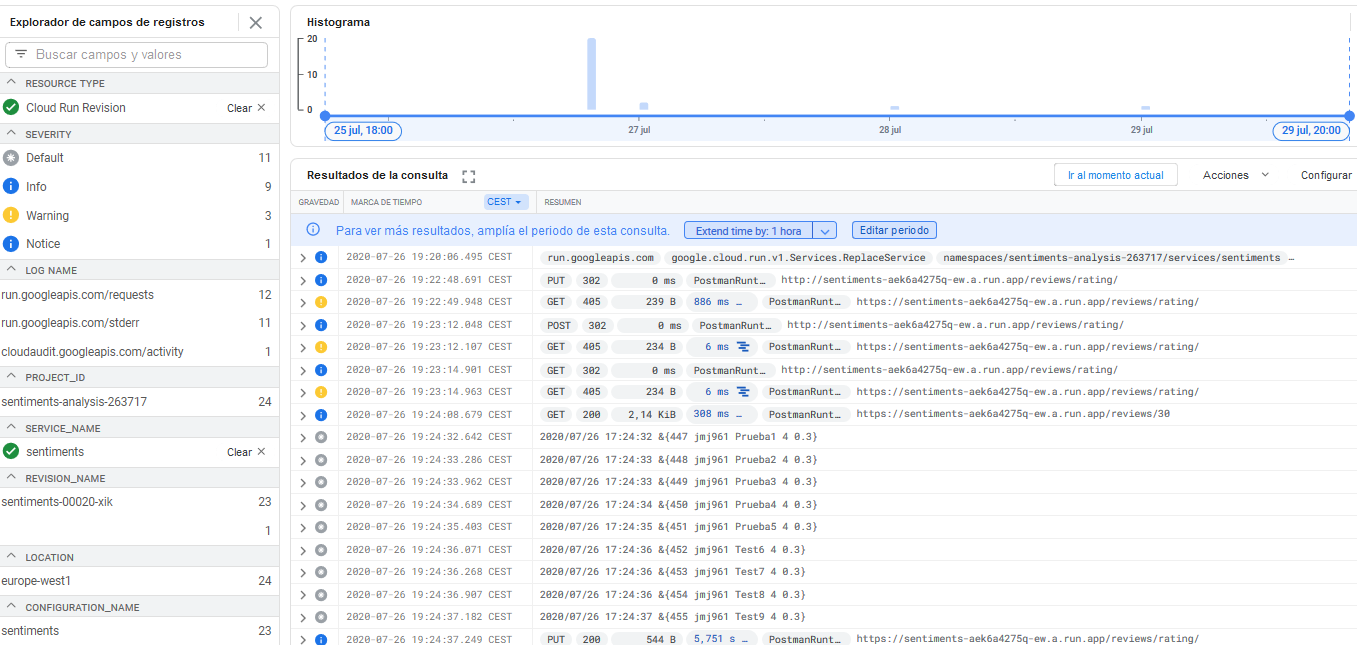
\includegraphics[width = 1\textwidth]{Figuras/cloudLogging.PNG}
	\end{center}
	\caption{\label{fig:cloudLogging} Visor de registros Cloud Logging}
\end{figure}

\newpage

Gracias a esta herramienta es posible gestionar y analizar los registros personalizados que se incluyen en la aplicación de análisis de sentimientos con el objetivo de identificar y solucionar rápidamente el origen de los posibles problemas que surjan.

\subsection{DialogFlow}

Se trata de una herramienta de Google Cloud que permite crear modelos que sean capaces de interpretar las intenciones del usuario y extraer información relevante de las conversaciones, todo ello a través de una interfaz de usuario visual que no requiere de experiencia en aprendizaje automático \citeW{DialogFlow}. 

\begin{figure}[ht]
     \begin{center}
        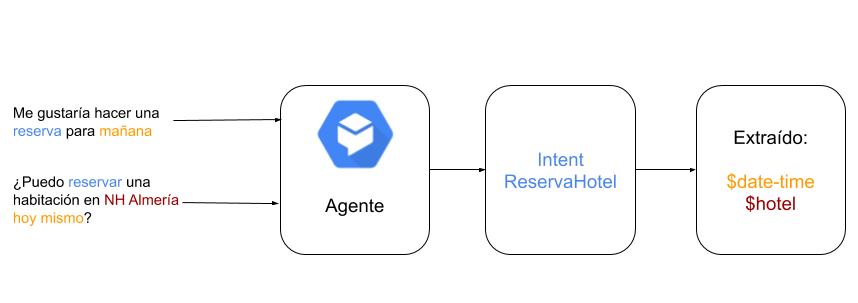
\includegraphics[width = 0.90\textwidth]{Figuras/IntentsDiagram.png}
     \end{center}
     \caption{\label{fig:IntentsDiagram}Diagrama de funcionamiento}
\end{figure}

\newpage

Para comprender su funcionamiento es necesario conocer los conceptos de:
\begin{itemize}
     \item \textbf{Agentes}. Se debe ver a un agente de DialogFlow como si se tratase, por ejemplo, de un trabajador en un centro de llamadas. Al igual que el empleado en sus primeros días de trabajo, el agente debe ser entrenado para manejar las conversaciones con los clientes. 
     
     DialogFlow traduce la entrada de texto que recibe por parte del usuario durante la conversación a datos estructurados que puedan ser utilizados por una aplicación o servicio.
    
     \item \textbf{Intents}. Básicamente es cómo determina DialogFlow lo que un usuario desea hacer. Permiten definir un conjunto de tareas individuales que pueden ser invocadas por el usuario. Es conveniente crear intents cuya funcionalidad esté centrada en el propósito de su creación, para que la duración de la invocación sea breve, ofreciendo así al usuario la respuesta adecuada en un intervalo de tiempo más corto.
     
     Un intent está formado por los siguientes elementos:
     \begin{itemize}
         \item Frases de entrenamiento. Son frases que el usuario puede decir para activar el intent. No es necesario definir todas las variantes posibles de una frase, ya que el aprendizaje automático que está integrado en la herramienta extiende la lista definida con otras frases parecidas.
         \item Acción. Cuando Dialogflow identifica una coincidencia con un intent, transmite la acción al sistema que puede ser usada para activar otras acciones definidas en el sistema. Por ejemplo, si el usuario pregunta acerca del estado de su pedido el agente reconoce la entidad pedido y pregunta por el número del mismo al usuario.  
         
         \begin{figure}[ht]
             \begin{center}
                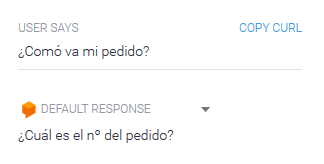
\includegraphics[width = 0.60\textwidth]{Figuras/Accion.PNG}
             \end{center}
             \caption{\label{fig:Accion}DialogFlow. Acción}
         \end{figure}
         
         \newpage
         
         \item Parámetros. Los valores extraídos cuando Dialogflow detecta una coincidencia se almacenan en forma de parámetros. Se trata de datos estructurados que permiten implementar alguna lógica o generar respuestas. Cada uno de ellos pertenece a un tipo de entidad, que determina cómo se realiza la extracción de los datos. 

         En el ejemplo anterior de un usuario preguntando por el estado de su pedido, si el usuario introduce el número de pedido el agente lo recoge en el parámetro \textit{@PedidoID}. Este hecho se ilustra a continuación:
         
          \begin{figure}[ht]
             \begin{center}
                \includegraphics[width = 0.85\textwidth]{Figuras/Parámetros.PNG}
             \end{center}
             \caption{\label{fig:DialogflowParams}DialogFlow. Parámetros}
          \end{figure}
         
         \item Respuestas. Son las contestaciones que el agente muestra al usuario. Éstas pueden responder a una pregunta del usuario, pedirle más información o dar por finalizada la conversación.
     \end{itemize}
     
     En el siguiente diagrama se puede observar cuál es el flujo para identificar coincidencias de intents y proporcionar una respuesta al usuario:
     
    
    
     
     \begin{figure}[ht]
         \begin{center}
            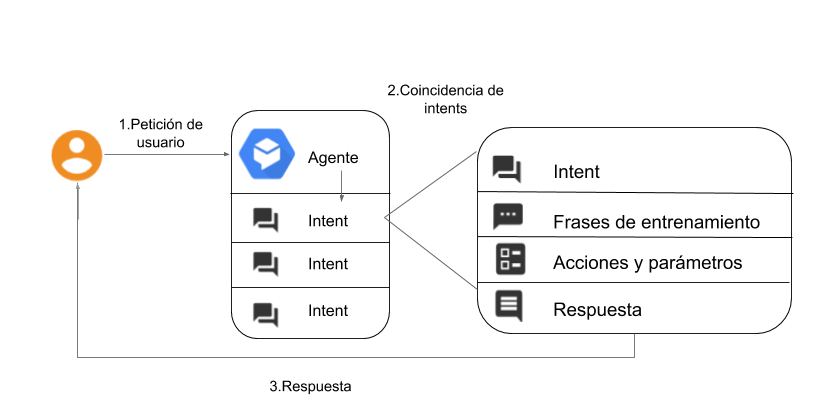
\includegraphics[width = 0.80\textwidth]{Figuras/FlujoCoincidencias.png}
         \end{center}
         \caption{\label{fig:FlujoCoincidencias}Flujo para identificar coincidencias y responder al usuario. Fuente: Google Cloud.}
     \end{figure}
     
     \newpage
     
     \item \textbf{Entidades}. Una entidad es una propiedad que Dialogflow utiliza para responder a una petición del usuario. Normalmente se trata de una palabra clave que contiene la petición como un nombre, fecha, localización, número, etc. Cuando el usuario realiza la petición, Dialogflow busca las entidades y extrae sus valores en forma de parámetros.
     
     Existe un conjunto predefinido de entidades del sistema para detectar coincidencias con muchos tipos comunes de datos. Si estas entidades no son suficientes, se pueden definir todas las entidades que se deseen para detectar coincidencias con datos personalizados. Por ejemplo, se puede definir la entidad PedidoID, como puede observarse en la siguiente figura:
     
     \begin{figure}[ht]
         \begin{center}
            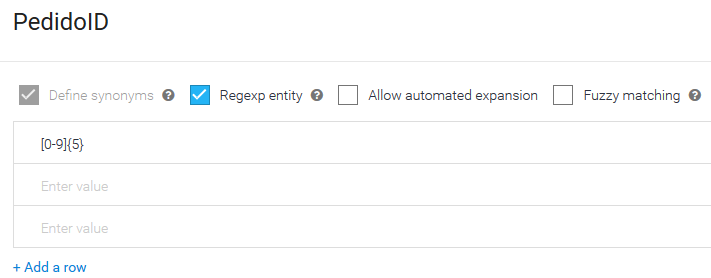
\includegraphics[width = 0.95\textwidth]{Figuras/Entidades.PNG}
         \end{center}
         \caption{\label{fig:DialogflowEntities}DialogFlow. Entidades}
     \end{figure}
     
     En la figura puede apreciarse que se ha definido una expresión regular para identificar los números de pedido.
     
     \newpage
     
     \item \textbf{Contextos}. Este concepto es semejante al usado en el lenguaje natural. Si una persona dice "es rojo", se necesita conocer el contexto para saber a qué se está refiriendo. De forma análoga, Dialogflow necesita un contexto para identificar el intent que se corresponde con la petición del usuario.
     
     Es un concepto importante, puesto que, permite tomar decisiones basadas en las respuestas anteriores, arreglar conversaciones que puede que se hayan roto por cualquier motivo y también ramificar la conversación en diferentes intents para crear una conversación fluida con el usuario.
     
     \item \textbf{Eventos}. Sirven para activar un intent sin que el usuario haga ninguna consulta. Por ejemplo, cuando el usuario abre el chat para comenzar una conversación con el bot se invoca al evento de bienvenida genérico "Welcome".
     
     \item \textbf{Fulfillments y Webhooks}. Permiten la comunicación del agente con otros servicios externos. Por defecto, el agente ofrece al usuario una respuesta predefinida en función del intent con el que se haya encontrado una coincidencia, sin embargo mediante los fulfillments el agente envía una solicitud al servicio webhook que tiene información sobre dicho intent. Un webhook no es más que un destino final en un servidor con el que se prevé contactar. De esta forma, el sistema realiza una acción determinada ante la petición efectuada por el agente y le responde con información sobre como proceder.
     
     Por ejemplo: si un usuario quiere reservar una habitación de hotel para Semana Santa, el servicio puede comprobar la base de datos y comunicarle al usuario si hay alguna habitación disponible en esas fechas.
     
     Para crear un webhook solo es necesario indicar la URL del destino final donde se van recoger las peticiones. Cada webook está asignado a un intent de modo que cuando se produce una coincidencia entre la entrada del usuario y dicho intent, se realizará una petición al servicio que incluirá en forma de JSON la información que el agente ha extraído del intent. 
     
     \begin{figure}[ht]
         \begin{center}
            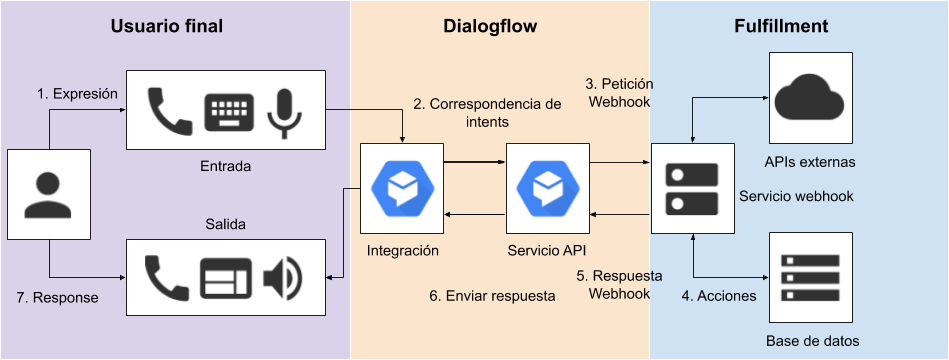
\includegraphics[width = 0.95\textwidth]{Figuras/Diagrama fulfillment.png}
         \end{center}
         \caption{\label{fig:DialogflowFulfillments}Flujo de fulfillment. Google Cloud.}
     \end{figure}
     
\end{itemize}
\chapter{Desarrollo} 
\label{sec:desarrollo}

\section{Arquitectura}

El desarrollo se ha llevado a cabo siguiendo un enfoque basado en microservicios. Comúnmente, las aplicaciones presentan una arquitectura monolítica, esto quiere decir que todos los elementos que se implementan se encuentran contenidos en una aplicación individual. Uno de los principales inconvenientes de este tipo de arquitectura es su rigidez. Solucionar problemas o actualizar la aplicación con nuevas funcionalidades en la aplicación se puede volver difícil y tedioso. 

Para hacer frente a los problemas que supone la arquitectura monolítica, surgió un nuevo tipo de arquitectura de microservicios, donde cada elemento o proceso son independientes y trabajan entre sí para conseguir la funcionalidad que requiere la aplicación. Básicamente, la aplicación se divide en servicios, donde cada uno es un proceso autónomo. La ventaja de este enfoque reside principalmente en este hecho, la independencia de los procesos, puesto que de esta forma es posible introducir cambios sin que ello conlleve ninguna modificación sobre el resto de los servicios. 

En la siguiente figura se comparan ambos tipos de arquitecturas:

\begin{figure}[ht]
	\begin{center}
		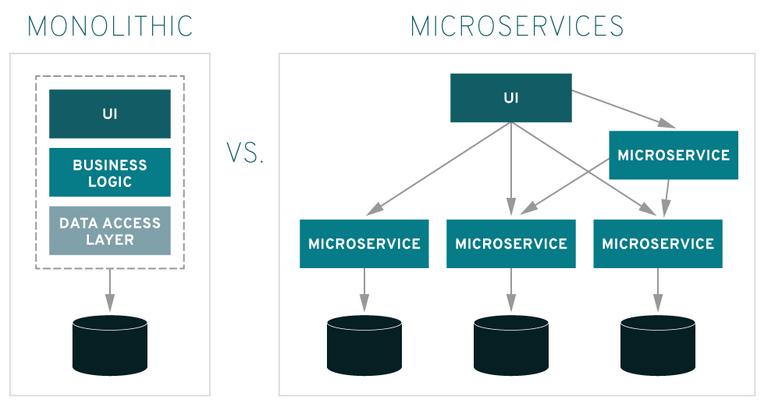
\includegraphics[width = 0.70\textwidth]{Figuras/microservicios.PNG}
	\end{center}
	\caption{\label{fig:microservicios} Comparación de la arquitectura monolítica y de microservicios. Fuente: Red Hat.}
\end{figure}

\newpage

La base del proyecto es una página web construida usando Wordpress. En ella se han incluido una herramienta de análisis de sentimientos y un bot conversacional. Estará conectada a un segmento de Cloud Storage. Aquí se almacenarán los contenidos importados durante su funcionamiento. 

Cuando un comentario es publicado en la página web, se realiza una llamada a la API de la aplicación de análisis de sentimientos para crear su valoración. El servicio encargado de esta acción recupera un comentario de la base de datos y envía una petición a la función adecuada de Natural Language. Por último, devuelve el resultado a Wordpress. Si ocurre algún error en el proceso, creará un nuevo registro en Cloud Logging.

Tanto esta aplicación como Wordpress se despliegan en Cloud Run utilizando contenedores que, previamente, han sido almacenados en Container Registry. Además, ambas usarán la misma instancia de la base de datos en Cloud SQL. 

Por su parte, la implementación del chatbot se ha realizado con Dialogflow, integrándolo en Wordpress mediante una extensión conocida como MyChatbot. Actualmente, no se encuentra conectado con la base de datos, pero se plantea que lo esté en el futuro.

En la siguiente figura se muestra la arquitectura del sistema:

\begin{figure}[ht]
	\begin{center}
		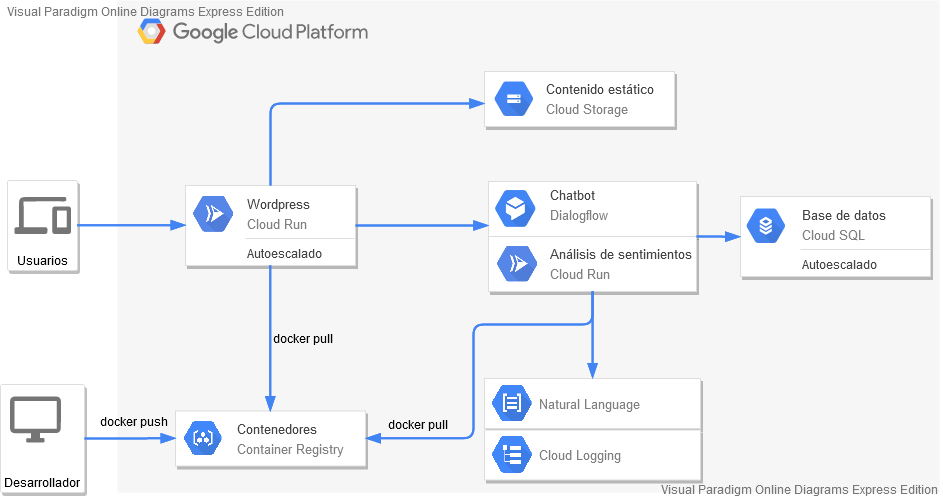
\includegraphics[width = 0.95\textwidth]{Figuras/ArquitecturaV3.png}
	\end{center}
	\caption{\label{fig:systemArchitecture} Arquitectura del sistema}
\end{figure}

\newpage
\section{Implementación}

En esta sección se describe con detalle el proceso que se ha seguido para poner en marcha cada uno de los elementos centrales que componen este proyecto. Se divide en tres subsecciones dedicadas a: página web, análisis de sentimientos y bot conversacional.

\subsection{Página web}

El sitio web se ha desarrollado con Wordpress en un servidor local. Tras finalizar el proceso, se ha introducido en un contenedor y se ha desplegado en la nube. A partir de este momento la página web ya está disponible para los usuarios.

El primer paso consiste en construir el entorno de desarrollo mediante XAMPP. Este programa ya es suficiente para disponer de un servidor web local preparado para alojar una página web. Cómo se puede apreciar en la siguiente figura sólo serán necesarios los módulos de Apache y MySQL:

\begin{figure}[ht]
	\begin{center}
		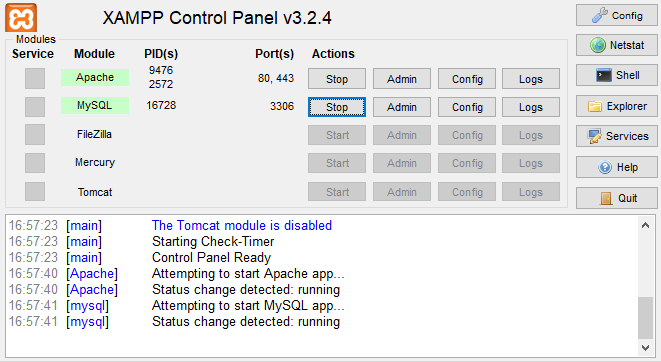
\includegraphics[width = 0.80\textwidth]{Figuras/XAMPP.PNG}
	\end{center}
	\caption{\label{fig:xampp} XAMPP en funcionamiento}
\end{figure}

Para su funcionamiento Wordpress requiere de una base de datos, por lo tanto, el siguiente paso consiste en crear una instancia en el servidor de MySQL de XAMPP. Con este objetivo se utiliza la aplicación de administración phpMyAdmin, que también está incluida en XAMPP. Dicha aplicación se puede visualizar en el navegador desde la dirección \textit{http://localhost/phpmyadmin/}. En la próxima figura se señala la instancia creada:

\begin{figure}[ht]
	\begin{center}
		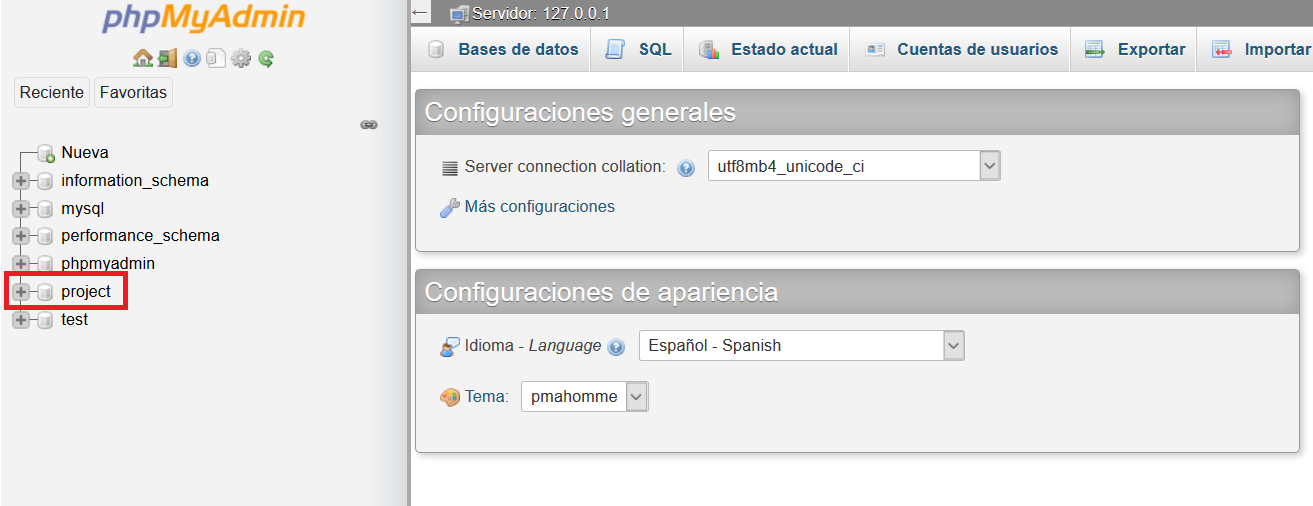
\includegraphics[width=15.93cm, height=6.14 cm, ]{Figuras/phpmyadmin.png}
	\end{center}
	\caption{\label{fig:phpmyadmin} Interfaz de phpMyAdmin}
\end{figure}
\newpage

Una vez hecho esto, se descarga Wordpress desde \url{https://wordpress.org/} y se extrae su contenido en la carpeta htdocs situada dentro del directorio de XAMPP. Esta carpeta es similar a la carpeta public\_html usada por la mayoría de hostings como raíz para la instalación de páginas webs.

Ya sólo queda acceder a la dirección \textit{http://localhost/wordpress/} y seguir los pasos que se van mostrando para finalizar el proceso de instalación.

Si el proceso se ha realizado correctamente se podrá acceder al panel de administración de Wordpress a través de la dirección \textit{localhost/wordpress/wp-admin/}. La siguiente imagen muestra el aspecto de dicho panel:

\begin{figure}[ht]
	\begin{center}
		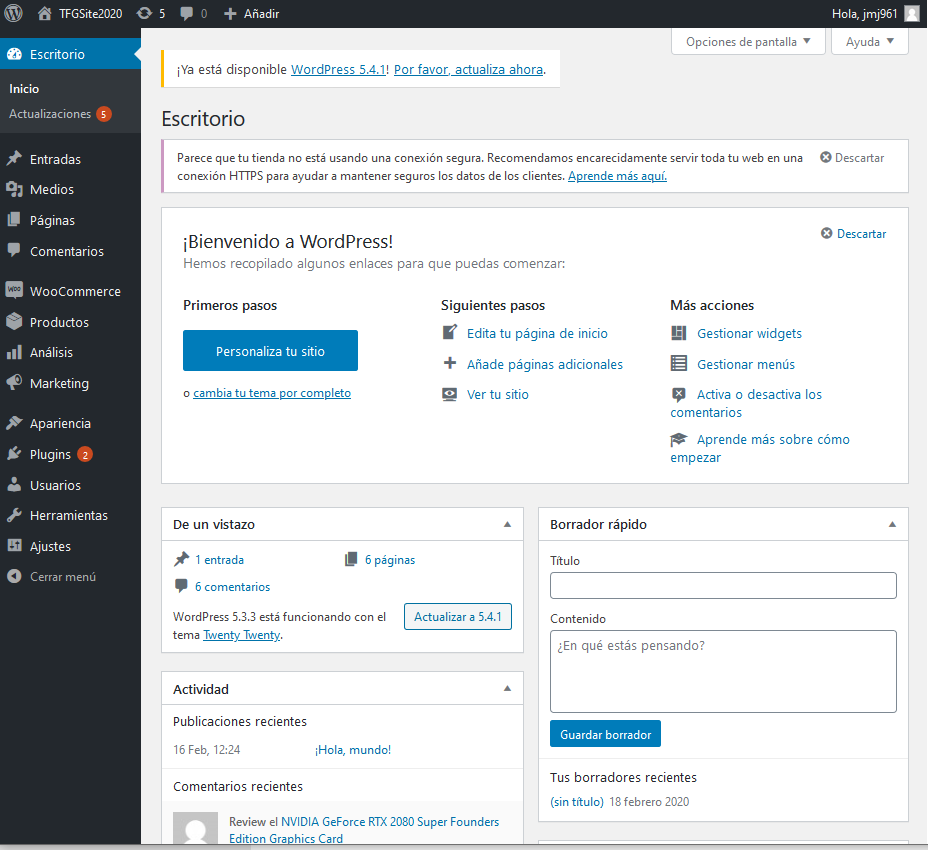
\includegraphics[width = 0.65\textwidth]{Figuras/wpadmin.PNG}
	\end{center}
	\caption{\label{fig:wordpressAdmin} Panel de administración Wordpress}
\end{figure}
\newpage

Ahora, se procede a instalar y configurar los plugins necesarios: WooCommerce, para transformar la página en una tienda de comercio electrónico; MyChatbot, para integrar el bot conversacional, y WP-Stateless, que permitirá otorgar persistencia a los archivos multimedia cargados a la página cuando se realice su despliegue en Cloud Run.

En el siguiente paso se introducen productos y comentarios que serán utilizados más adelante para comprobar el funcionamiento de la aplicación de análisis de sentimientos. Tanto los productos como sus comentarios son ejemplos reales extraídos de Amazon y PcComponentes.

Por último, se modificará el diseño del sitio con la intención de que resulte más atractivo a los usuarios. Con esta idea, se ha utilizado la versión gratuita de la extensión Elementor, que simplifica considerablemente dicha tarea. La explicación de este proceso se va a obviar por considerarse que queda fuera a los objetivos de este trabajo. La siguiente imagen muestra uno de los productos ofertados en la página web:

\begin{figure}[ht]
	\begin{center}
		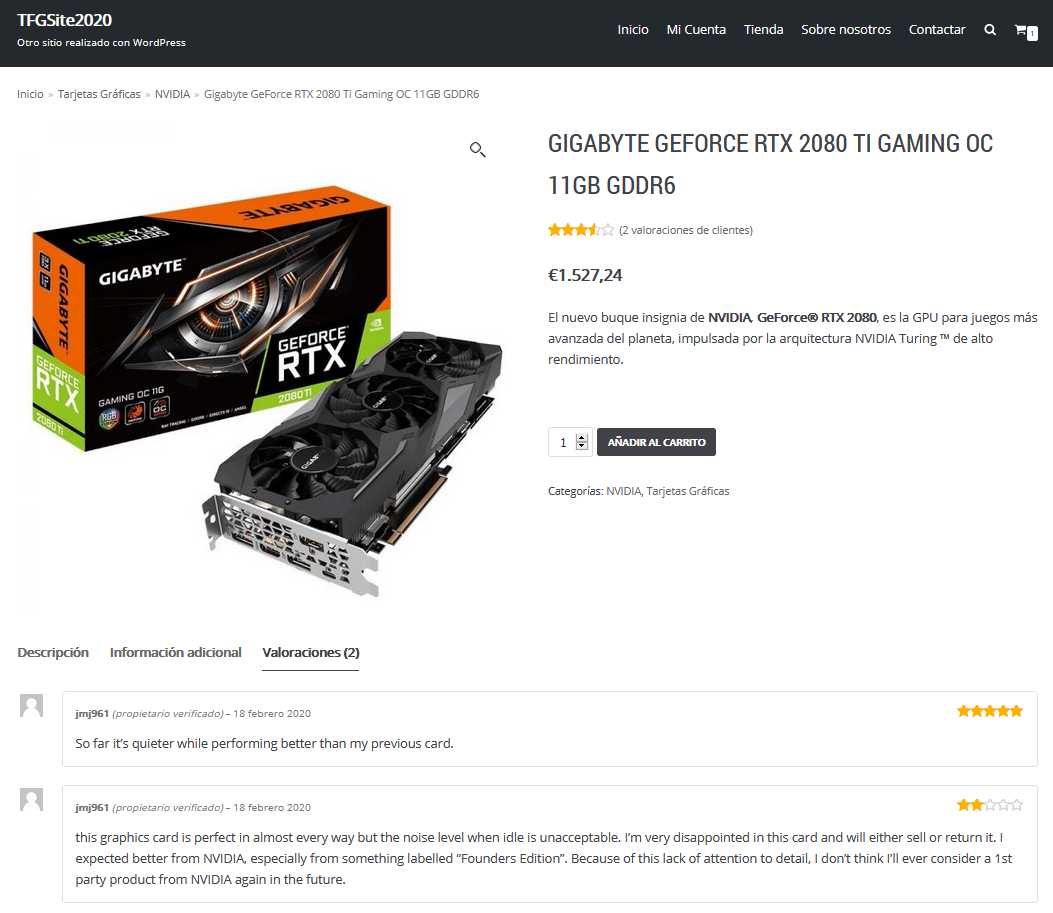
\includegraphics[width = 0.80\textwidth]{Figuras/tiendaWordpress.PNG}
	\end{center}
	\caption{\label{fig:tienda} Tarjeta gráfica ofertada en la página web}
\end{figure}
\newpage

\subsection{Análisis de sentimientos}

El análisis de opiniones de los comentarios que los usuarios publican en el sitio web se realiza mediante una aplicación desarrollada en GoLang. Ésta actúa como envoltorio del servicio de procesamiento del lenguaje natural ofrecido por Google a través de su nube. Todo el código de la aplicación está disponible en \url{https://github.com/jo4nymj/sentiment-analysis}. El proyecto presenta la siguiente estructura:
\begin{itemize}
    \item \textbf{Paquetes}
    \begin{itemize}
        \item \textbf{database}. Establece la conexión con la base de datos. Se ha optado por implementar un patrón de diseño Singleton para que exista una única instancia de la base de datos a la que se accede a través de un punto de acceso global. Para establecer una conexión con la base de datos desde otro paquete basta con hacer referencia a la variable \textit{Instance}. 
        
        \begin{lstlisting}[caption= Singleton]
        var Instance *Connection
        func init() {
        	if Instance == nil {
        		Instance = GetMySQLDB() // Devuelve &Connection{Conn: db}
        	}
        }
        type Connection struct {
        	Conn *sql.DB
        }
        \end{lstlisting}
        
        En Go, la función init() se ejecuta antes que cualquier otro fragmento del código del paquete donde se incluya la función. Por tanto, se ejecutará en el momento en el que se importe el paquete.
        
        \item \textbf{config}. Aquí se incluyen las variables de configuración relacionadas con la conexión a la BBDD y a la generación del token de seguridad que se utiliza en las peticiones. Se comprueba si el entorno en el que se está ejecutando la aplicación es local o producción y, en función de ello se asignan valores a las variables.
        
        \item \textbf{logger}. Crea e inicializa un cliente para establecer la comunicación con el servicio de Cloud Logging. Del mismo modo, implementa las funciones que se utilizarán para realizar el envío de los registros: \textit{Print} y \textit{Error}.
        
        \item \textbf{models}. Es necesario un modelo para los comentarios y otro para los productos. En Go no existen las clases, pero se puede conseguir que los structs utilizados para crear los modelos actúen como tal asignándoles métodos. Seguidamente se expone el diagrama de clases:
        
        \begin{figure}[ht]
        	\begin{center}
        		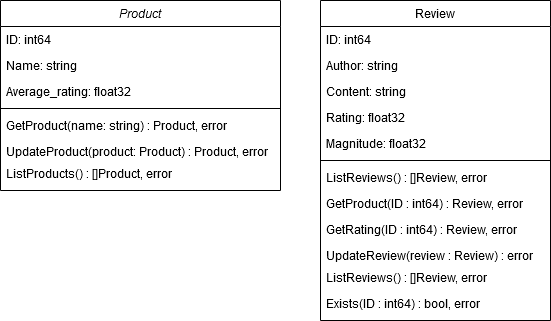
\includegraphics[width=0.80\textwidth]{Figuras/DiagramaClases.png}
        	\end{center}
        	\caption{\label{fig:classDiagram} Diagrama de clases}
        \end{figure}
        
        \newpage
        
        Ha sido necesario introducir modificaciones en el modelo de comentario con el que trabaja WooCommerce. De forma predeterminada, se crean dos entradas asociadas a un comentario en la tabla \textit{wp\_commentmeta}. Una de estas entradas sirve para identificar si un comentario está verificado, si no lo está, éste no será mostrado a los usuarios de la página web. La otra entrada es utilizada por Wordpress para almacenar la valoración que un usuario introduce junto a su comentario (\textit{meta\_value}). Por tanto, como Google NLP devuelve dos valores (puntuación y magnitud), se ha decidido reutilizar el campo de \textit{meta\_value} para asignar la puntuación y añadir una nueva columna para la magnitud. En la siguiente figura se muestra parte del contenido de la tabla \textit{wp\_commentmeta}:
        
        \begin{figure}[ht]
        	\begin{center}
        		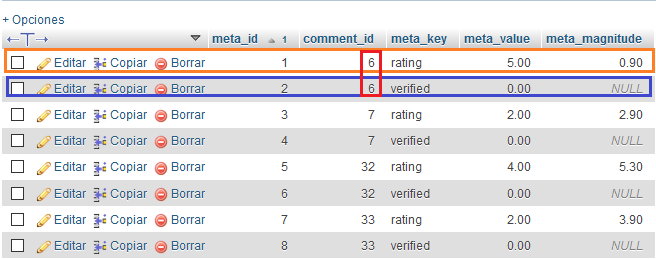
\includegraphics[width = 0.95\textwidth]{Figuras/wp_commentmeta.PNG}
        	\end{center}
        	\caption{\label{fig:commentmeta} Tabla wp\_commentmeta}
        \end{figure}
        
        \newpage 
        
        En naranja se ha señalado la entrada correspondiente a la evaluación del comentario y en azul la que corresponde al estado de verificación. Se puede identificar claramente a qué corresponde cada entrada si se observa el valor de la columna \textit{meta\_key}. En rojo se resalta que ambas entradas se refieren al mismo comentario puesto que comparten el valor de \textit{comment\_id}.
        
        \item \textbf{repository}. Aquí se definen los métodos asociados a los modelos donde se realizan operaciones sobre la base de datos como extraer, actualizar o ingresar datos.
        
        \item \textbf{services}. Se han implementado métodos que permiten interactuar con los productos y sus comentarios para poder crear  y actualizar los modelos, así como recuperar información sobre ellos. 
        
        En relación a los productos se han implementado dos métodos:
        \begin{itemize}
            \item \textbf{Obtener un producto}. Dado el nombre de un producto permite obtener de la base de datos su información.
            \item \textbf{Actualizar un producto}. A partir del nombre de un producto, fuerza la actualización de su puntuación. Para ello, recorre sus comentarios y obtiene la media de puntuación. De forma normal, Wordpress actualiza la puntuación del producto cada vez que se evalúa una nueva opinión. Aún así, en algunas ocasiones este proceso puede presentar fallos y no actualizar correctamente la información, por lo que se ha visto conveniente implementar este método para atajar posibles problemas.
        \end{itemize}
        
        En cuanto a las opiniones o comentarios se han definido los siguientes métodos:
        \begin{itemize}
            \item \textbf{Listar opiniones}. Dado el id de un producto se listan todos sus comentarios, conteniendo la información sobre su valoración.
            \item \textbf{Crear valoración de una opinión}. A partir del identificador de un comentario, extrae su información de la base de datos; si aún no ha sido evaluado, realiza una llamada a la API de Google para hacerlo y almacena el resultado.
            \item \textbf{Actualizar opiniones}. Fuerza la llamada a la API de Google para actualizar los valores de puntuación y magnitud de un comentario específico.
        \end{itemize}
        
        \newpage
        
        A continuación, se muestra un diagrama que modela las interacciones con la API:
        
         \begin{figure}[ht]
        	\begin{center}
        		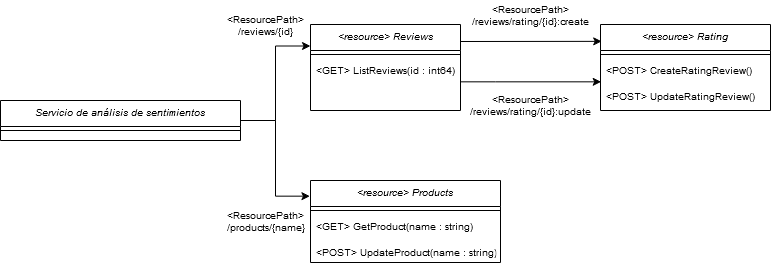
\includegraphics[width = 0.95\textwidth]{Figuras/DiagramaAPI.png}
        	\end{center}
        	\caption{\label{fig:modelAPI} Modelo de la API}
        \end{figure}
    \end{itemize}
    \item \textbf{Ficheros}
     \begin{itemize}
        \item \textbf{main}. En este fichero se establecen las URLs de acceso a cada uno de los servicios y el puerto a través del cual se realizará la comunicación.
        \item \textbf{go.mod}. Incluye los módulos con los que el proyecto presenta dependencias.
        \item \textbf{go.sum}. En este fichero se encuentran los hashes criptográficos de las versiones específicas de los módulos.
        \item \textbf{Dockerfile}. Contiene las instrucciones para crear la imagen del contenedor. Su implementación se explicará más adelante en la subsección 6.3.2.
    \end{itemize}
\end{itemize}

Tras haber expuesto de manera general la estructura del proyecto y haber hablado brevemente sobre la función de cada uno de sus componentes, resulta conveniente tratar con más profundidad el método destinado a crear valoraciones de un comentario. 

Hay algo que se debe tener en cuenta para entender la manera en la que se ha construido este método. Como ya se explicó anteriormente en la subsección 4.1.1, por defecto se requiere al usuario introducir una valoración junto con su comentario a través de un componente gráfico con forma de estrellas. Esta funcionalidad ha sido modificada para que no sea el usuario quien introduzca dicha valoración, sino que ésta venga dada por la evaluación de Google NLP. El comentario será almacenado en un primer momento en la tabla \textit{wp\_comment} sin valoración, por lo tanto la tabla \textit{wp\_commentmeta} no contará con una entrada destinada a su puntuación. Será el método \textit{CreateRatingReview} el encargado de crear dicha entrada en la tabla de \textit{wp\_commentmeta}. Seguidamente se muestra el diagrama de secuencia que modela el proceso para crear una valoración:

\begin{figure}[ht]
	\begin{center}
		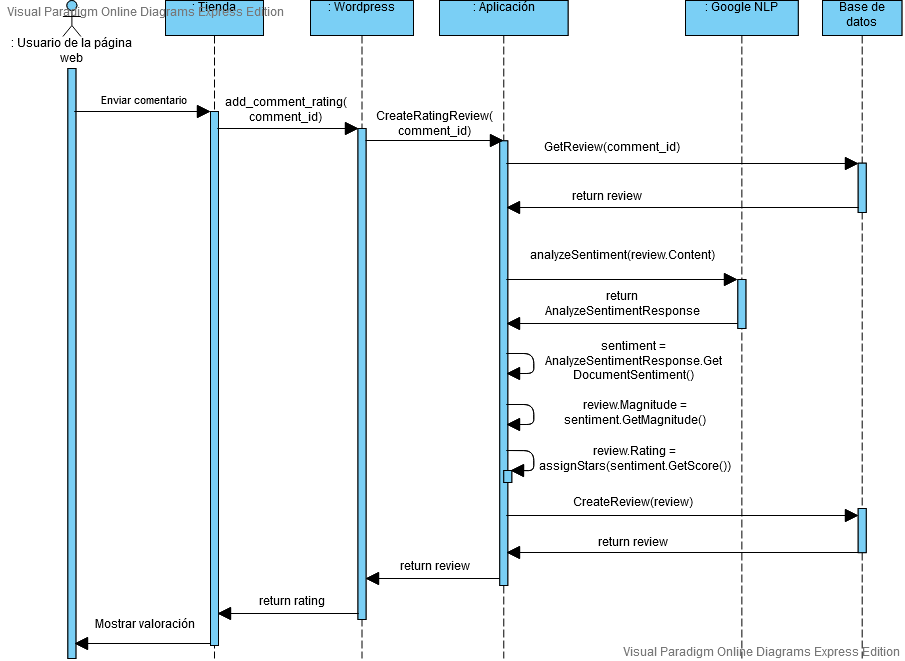
\includegraphics[width = 1\textwidth]{Figuras/DiagramaSecuencia.png}
	\end{center}
	\caption{\label{fig:sequenceDiagram} Diagrama de secuencia CreateRatingReview}
\end{figure}
\newpage
Tras esto se procede a presentar la implementación del mismo:
\begin{lstlisting}[caption= M\'etodo para crear una valoraci\'on de un comentario]
func CreateRatingReview(w http.ResponseWriter, r *http.Request) {
	reviewModel := repository.ReviewModel{
		Db: database.Instance,
	}
	reviewID, err := strconv.ParseInt((mux.Vars(r)["id"]), 10, 64)
	if err != nil {
		logger.Error("Failed to parse the ID of the review, %v", err)
		utilities.StatusInternalServerError(w, r)
	}
	exists, err := reviewModel.Exists(reviewID)
	if err != nil {
		logger.Error("Failed to retrieve the review from the database, %v", err)
		utilities.StatusBadRequest(w, r, "")
	}
	if exists {
		utilities.StatusBadRequest(w, r, "Review already exists")
		return
	}
	review, err := reviewModel.GetReview(reviewID)
	if err != nil {
		logger.Error("Failed to retrieve the review from the database, %v", err)
		utilities.StatusBadRequest(w, r, "")
	}
	if err := analyze(&review); err != nil {
		logger.Error("Failed to analyze the review, %v", err)
		utilities.StatusInternalServerError(w, r)
	}
	if err := reviewModel.CreateReview(review); err != nil {
		logger.Error("Failed to create review: %v", err)
		utilities.StatusBadRequest(w, r, "")
	}
	json.NewEncoder(w).Encode(review)
}
\end{lstlisting}

En primer lugar se extrae el identificador del comentario incluido en la petición. A partir de este parámetro se comprueba si el comentario ya tiene una valoración registrada, en cuyo caso se responde a la petición con un estado 400, si no, se llama al método \textit{GetReview()} para obtener su entrada de la tabla \textit{wp\_comment}.

Posteriormente se procede a invocar a la función \textit{analyze()} dónde será evaluado el contenido del comentario. Esta función se ha construido de la siguiente forma:

\begin{lstlisting}[caption= Funci\'on que envuelve la llamada a la API de NLP]
func analyze(review *models.Review) error {
	ctx := context.Background()
	client, err := language.NewClient(ctx)
	if err != nil {
		return err
	}
	v, err := analyzeSentiment(ctx, client, review.Content)
	if err != nil {
		return err
	}
	sentiment := v.GetDocumentSentiment()
	review.Rating = assignStars(sentiment.GetScore())
	review.Magnitude = sentiment.GetMagnitude()

	return nil
}
\end{lstlisting}

La función comienza por crear un contexto y un cliente para establecer la comunicación con el servicio de destino. Un contexto en Golang es una forma de transmitir información entre una API y los procesos, información como: plazos máximos (deadlines), señales de cancelación y otros valores de alcance de la solicitud. 

Después se invoca a la API NLP desde la función \textit{analyzeSentiment()} pasando como parámetros un contexto, un cliente y el texto a evaluar. En el siguiente listado se puede apreciar como la función utiliza el cliente para invocar el servicio escogido de NLP y construye una petición con el texto a evaluar. 

\begin{lstlisting}[caption= Llamada a la API de NLP]
func analyzeSentiment(ctx context.Context, client *language.Client, text   string) (*languagepb.AnalyzeSentimentResponse, error) {
    return client.AnalyzeSentiment(ctx, &languagepb.AnalyzeSentimentRequest{
	Document: &languagepb.Document{
		Source: &languagepb.Document_Content{
			Content: text,
		},
		Type: languagepb.Document_PLAIN_TEXT,
	},
    })
}
\end{lstlisting}

La respuesta proporcionada por el servicio tiene la siguiente estructura:

\begin{lstlisting}[caption= Respuesta del servicio de NLP]
type AnalyzeSentimentResponse struct {
    // El sentimiento general del texto introducido
    DocumentSentiment *Sentiment
    // El lenguaje del texto, coincide con el especificado en la petición.
    // Si no fue especificado, es detectado automáticamente.
    Language string
    // El sentimiento de cada una de las frases del texto.
    Sentences []*Sentence
}
\end{lstlisting}
Para exponer este servicio, Google ha hecho uso de gRPC un proyecto open source desarrollado por ellos mismos. Está construido a partir del protocolo RPC (remote procedure call), permitiendo de este modo llamar desde una aplicación cliente a un servicio que se encuentre definido en un servidor como si se invocara a un procedimiento local. De forma simplificada la idea consiste en definir servicios compuestos por una serie de métodos RPC donde se especifican los mensajes de entrada que reciben y los mensajes de salida que generan.

\begin{figure}[ht]
\begin{center}
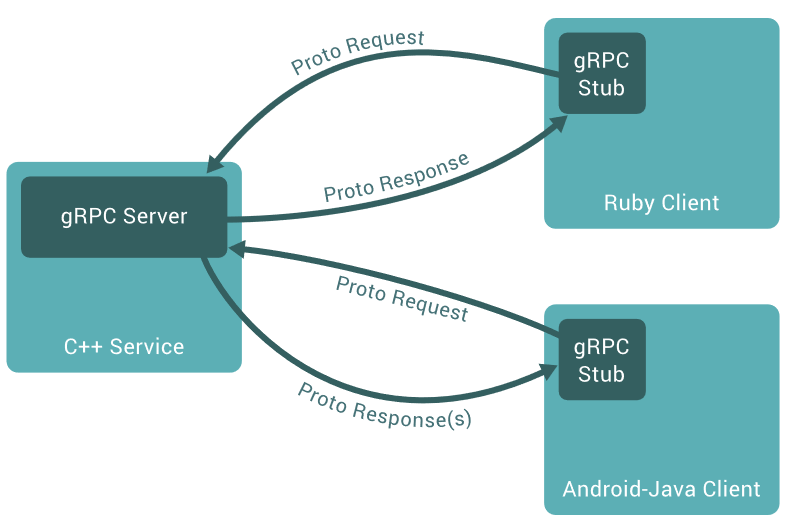
\includegraphics[width = 0.80\textwidth]{Figuras/gRPC.PNG}
\end{center}
\caption{\label{fig:grpc} Sistema gRPC. Fuente: gRPC.io.}
\end{figure}

Por defecto gPRC hace uso de Protocol Buffers o Protobuf para definir los servicios y los mensajes. Se trata un formato binario creado por Google para la serialización de información entre servicios. Actualmente, el formato más usado para este objetivo es JSON, sin embargo, Protobuf ofrece un mejor rendimiento, una mejor capacidad de mantenimiento y un tamaño más pequeño. Google proporciona un generador de código para los principales lenguajes de programación como, JavaScript, Java, PHP, C\#, Ruby, Objective C, Python, C++ y Go. Además Protobuf dispone de más tipos de datos que JSON, como enumeraciones y métodos.

Por este motivo la función \textit{analyzeSentiment} contiene una referencia a \textit{*languagepb}, que no es más que la definición del servicio haciendo uso de Protobuf.

Antes de almacenar el resultado de la petición se discretiza el campo Score (la puntuación) mediante la función \textit{assignStars()}. Esta función consiste en un switch donde se establece la cantidad de estrellas que corresponde  a un intervalo decimal específico, como se puede observar a continuación:

\begin{lstlisting}[caption= Funci\'on para discretizar la puntuaci\'on de una valoraci\'on]
func assignStars(rating float32) float32 {
	switch {
	case rating >= -1.0 && rating < -0.7:
		return 1.0
	case rating >= -0.7 && rating < -0.3:
		return 2.0
	case rating >= -0.3 && rating < 0.3:
		return 3.0
	case rating >= 0.3 && rating < 0.7:
		return 4.0
	case rating >= 0.7 && rating <= 1.0:
		return 5.0
	default:
		return 0.0
	}
}
\end{lstlisting}
    
Finalmente, se invoca al método CreateReview que se encarga de insertar la valoración del comentario en la tabla de \textit{wp\_commentmeta}.

\newpage

\subsubsection{Integración}

Se deben realizar las siguientes modificaciones en el backend de Wordpress:
\begin{enumerate}
\item \textbf{No requerir una valoración}. Se elimina el código existente desde la línea 122 a la 133 del fichero \textit{single-product-reviews.php}. De esta forma, ya no se exige al usuario introducir una valoración y tampoco se muestra el campo para hacerlo cuando éste escribe el comentario. El fragmento de código descartado es:

     \begin{lstlisting}[caption= No requerir una valoraci\'on al introducir un comentario]
if ( wc_review_ratings_enabled() ) {
	$comment_form['comment_field'] = '<div class="comment-form-rating"><label for="rating">' . esc_html__( 'Your rating', 'woocommerce' ) . '</label><select name="rating" id="rating" required>
		<option value="">' . esc_html__( 'Rate&hellip;', 'woocommerce' ) .'</option>
		<option value="5">' . esc_html__( 'Perfect', 'woocommerce' ) . '</option>
		<option value="4">' . esc_html__( 'Good', 'woocommerce' ) . '</option>
		<option value="3">' . esc_html__( 'Average', 'woocommerce' ) . '</option>
		<option value="2">' . esc_html__( 'Not that bad', 'woocommerce' ).'</option>
		<option value="1">' . esc_html__( 'Very poor', 'woocommerce' ) . '</option>
	</select></div>';
}
    \end{lstlisting}
\item  \textbf{Invocar al servicio de análisis de sentimientos}. Las valoraciones de los comentarios son añadidas por la función \textit{add\_comment\_rating()} que se encuentra en el fichero \textit{class-wc-comments.php} en la línea 161. Al principio de esta función se debe realizar una llamada al método de la API encargado de crear la valoración de un comentario, tal y como se muestra a continuación: 
    \begin{lstlisting}[caption= Llamar desde Wordpress al servicio de an\'alisis de sentimientos]
        $sentiment_api_url = 'http://localhost:5002/reviews/rating/' . $comment_id . ':create';
		$headers = array (
			'Authorization' => 'Bearer ' . getenv('TOKEN')
		);
		$args = array(
			'method' => 'POST',
			'headers' => $headers,
		);
		$response = wp_remote_request( $sentiment_api_url, $args );
    \end{lstlisting}
\end{enumerate}

Se realizará una petición de tipo POST a la dirección expuesta incluyendo en la cabecera un token de verificación que autorice la llamada a dicho servicio. Sólo se requerirá autorización al usuario de la API cuando se despliegue la aplicación en la nube, por lo que en local este parámetro será ignorado. Es importante sustituir la URL actual por la que corresponda cuando la aplicación sea desplegada.

\newpage

\subsection{Bot conversacional}

Desarrollar un bot conversacional para automatizar un proceso de negocio complejo, como el servicio de atención al cliente, no es una tarea sencilla. Las conversaciones poco comunes son muy difíciles de estructurar, ya que necesitan de un árbol de decisiones con cientos de declaraciones condicionales y encadenadas.

Por ejemplo, si se desea modelar una conversación que cuenta con 2 preguntas y 3 posibles respuestas harán falta 12 intents. Sin embargo, para modelar una conversación más realista, considerando un total de 10 preguntas con 2 posibles respuestas, supondría un total de 2047 intents. Aunque no sea necesario alcanzar ese número porque la conversación no va a tomar todas las posibles opciones, aún es necesaria una cantidad importante de intents.

Este trabajo tan sólo pretende mostrar el potencial que tiene la implementación de un bot conversacional en una tienda de comercio electrónico. Por tanto, se ha optado por implementar un bot para modelar procesos sencillos tales como la búsqueda de productos, ofrecer recomendaciones y resolver preguntas específicas. 

Al estrechar el dominio de la conversación limitando las opciones del cliente, se consigue reducir la complejidad de implementación, pero el usuario perderá la sensación de estar hablando con otra persona.

\subsubsection{Flujos de conversación}

En primer lugar, hay que definir los flujos de conversación que puede generar el usuario final. En este caso se ha identificado cada flujo de conversación con una de las funcionalidades del chatbot. A la hora de diseñar el trascurso de la conversación se han mezclado dos estilos: en algunos momentos el agente simplemente solicita al usuario final que seleccione una de las opciones que se le presentan mediante el uso de botones, mientras que en otros, se deja libertad al usuario para introducir la entrada de texto que considere oportuna.

A continuación, se va a describir cada uno de estos flujos adjuntando un diagrama que sirva como ejemplo para ilustrar la conversación entre el usuario (naranja) y el agente (azul). Las frases introducidas por el usuario que aparecen entren comillas indican entradas variables, es decir, se espera que el usuario pueda introducir cualquier entrada de texto. Por el contrario, cuando no aparece entrecomillada indica que la entrada se realiza a partir de una selección presentada por el agente (pulsar el botón correspondiente a la opción).

\begin{itemize}
    \item \textbf{Buscar un producto}. Su finalidad es que el usuario obtenga un enlace al catálogo de productos deseado. El agente le preguntará por el tipo de producto y la marca del mismo. A partir de las opciones escogidas por el usuario, el agente le responderá con un enlace al catálogo de dichos productos.
    \begin{figure}
    \begin{center}
    	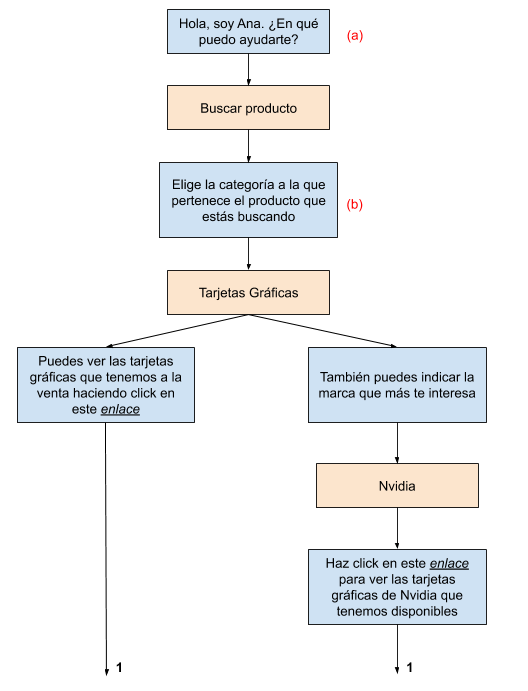
\includegraphics[width = 0.60\textwidth]{Figuras/Buscar producto (1).png}
    	\caption{\label{fig:buscarProducto1} Flujo de conversación para Buscar un producto. Parte I}
    	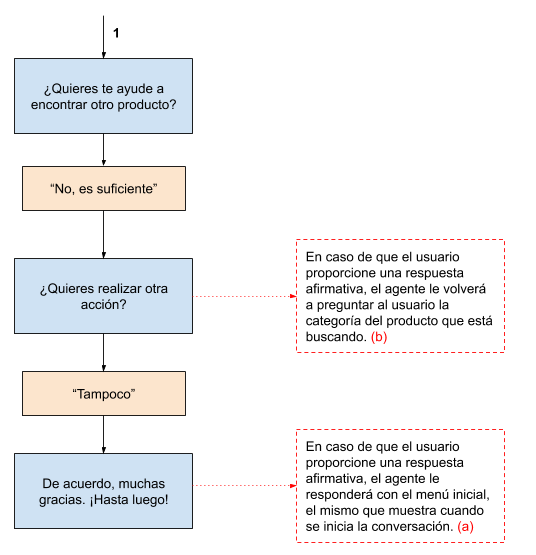
\includegraphics[width = 0.60\textwidth]{Figuras/Buscar producto (2).png}
    	\caption{\label{fig:buscarProducto2} Flujo de conversación para Buscar un producto. Parte II}
	\end{center}
    \end{figure}
    
    \newpage

    \item \textbf{Pedir una recomendación}. El agente pide al usuario que seleccione el tipo de producto y su marca, y según esta información recomienda el producto mejor valorado por los clientes que cumpla con los requisitos establecidos. 
    
    \begin{figure}
    	\begin{center}
    		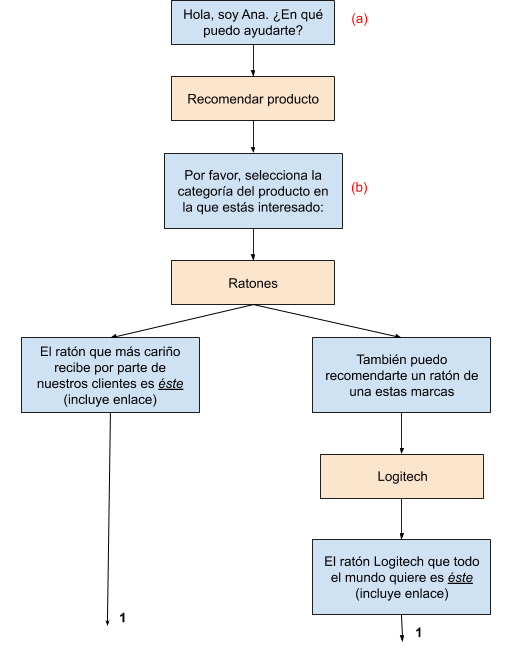
\includegraphics[width = 0.60\textwidth]{Figuras/Recomendar producto (1).png}
    		\caption{\label{fig:recomendarProducto1} Flujo de conversación para Pedir una recomendación. Parte I}
    		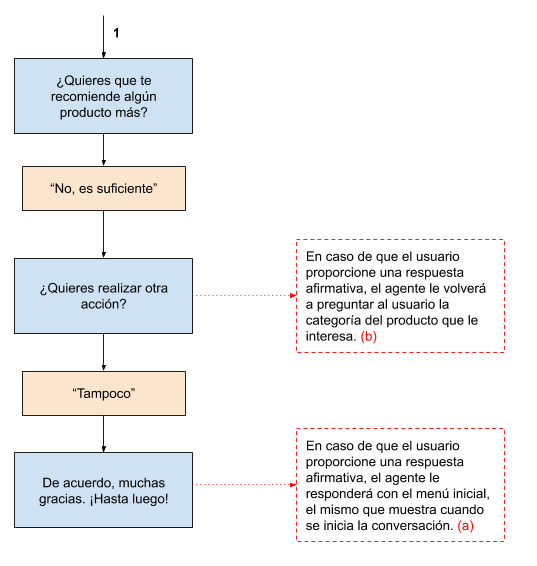
\includegraphics[width = 0.60\textwidth]{Figuras/Recomendar producto (2).png}
    		\caption{\label{fig:recomendarProducto2} Flujo de conversación para Pedir una recomendación. Parte II}
    	\end{center}
    \end{figure}
\newpage
    \item \textbf{Pedir un agente humano}. Si el usuario desea ponerse en contacto con un empleado de la empresa puede iniciar este flujo de conversación. El agente le proporcionará un enlace al formulario para contactar con el servicio de atención al cliente.
    \begin{figure}[ht]
    	\begin{center}
    		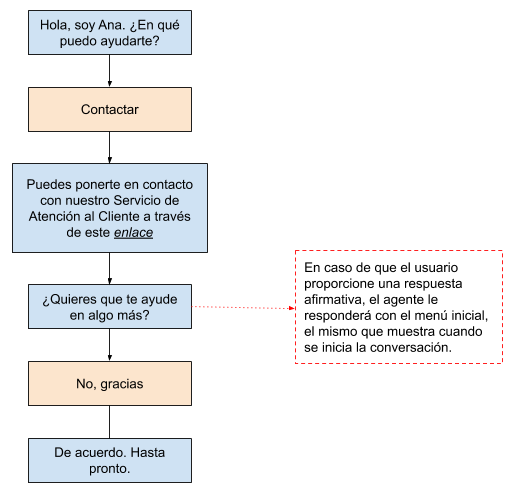
\includegraphics[width = 0.60\textwidth]{Figuras/Contactar.png}
    	\end{center}
	\caption{\label{fig:contactarAgente} Flujo de conversación para Solicitar un agente humano}
    \end{figure}
    
    \item \textbf{Realizar una consulta genérica}. El usuario puede realizar diversas preguntas relacionadas con el servicio de atención al cliente. Suelen estar resueltas en el apartado de preguntas frecuentes que se puede encontrar en la mayoría de tiendas online. Por ejemplo: preguntar acerca de las medidas que la empresa ha tomado ante el coronavirus, garantías, plazos de entrega, medios de pago, etc.
    \begin{figure}[ht]
    	\begin{center}
    		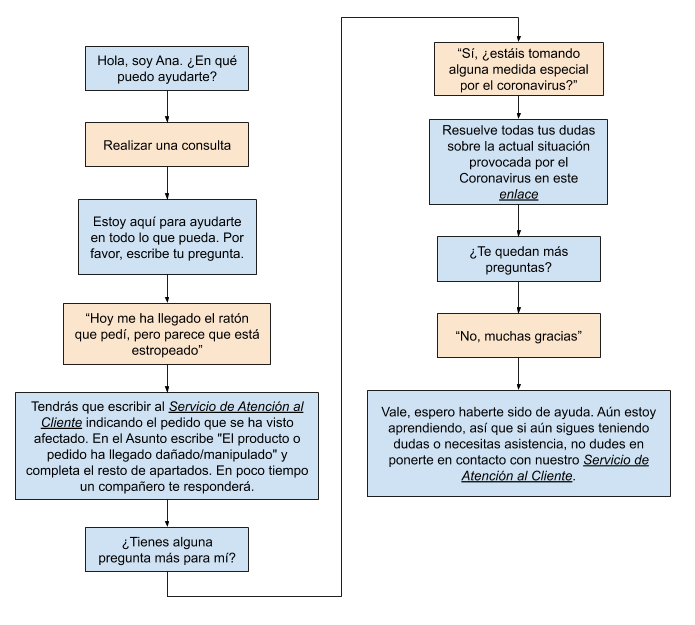
\includegraphics[width = 0.80\textwidth]{Figuras/Realizar consulta.png}
    	\end{center}
	\caption{\label{fig:realizarConsulta} Flujo de conversación para Realizar una consulta genérica}
    \end{figure}

\newpage
    
    \item \textbf{Comprobar el estado del pedido}. El agente pregunta al usuario cuál es el número del pedido sobre el que desea realizar la consulta. En este proyecto, el agente simplemente ofrece una respuesta predefinida, aunque en el futuro sería conveniente que se ligara esta pregunta a una consulta realizada sobre la base de datos. El número de pedido se ha definido como una entidad, por lo que el agente es capaz de extraerlo de la entrada de datos y almacenarlo en un variable.
    \begin{figure}[ht]
    	\begin{center}
    		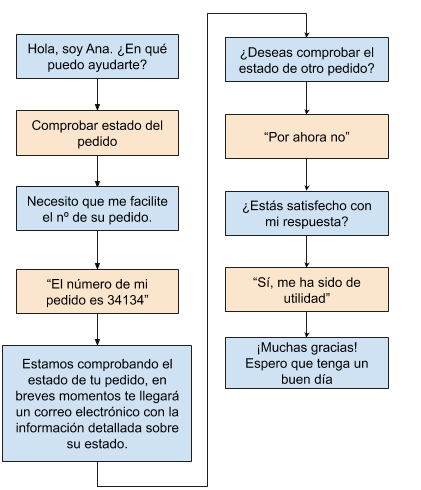
\includegraphics[width = 0.60\textwidth]{Figuras/Comprobar estado del pedido.png}
    	\end{center}
	\caption{\label{fig:estadoPedido} Flujo de conversación Comprobar estado del pedido}
    \end{figure}
\newpage

\end{itemize}

\subsubsection{Intents}

Se han creado diferentes intents para soportar cada flujo de conversación que se puede dar entre el agente y el usuario. Estas intenciones tienen que ver con el saludo, la búsqueda y recomendación de productos, conocer el estado de un pedido y el servicio de atención al cliente. En la siguiente figura se pueden observar los intents principales:

\begin{figure}[ht]
	\begin{center}
		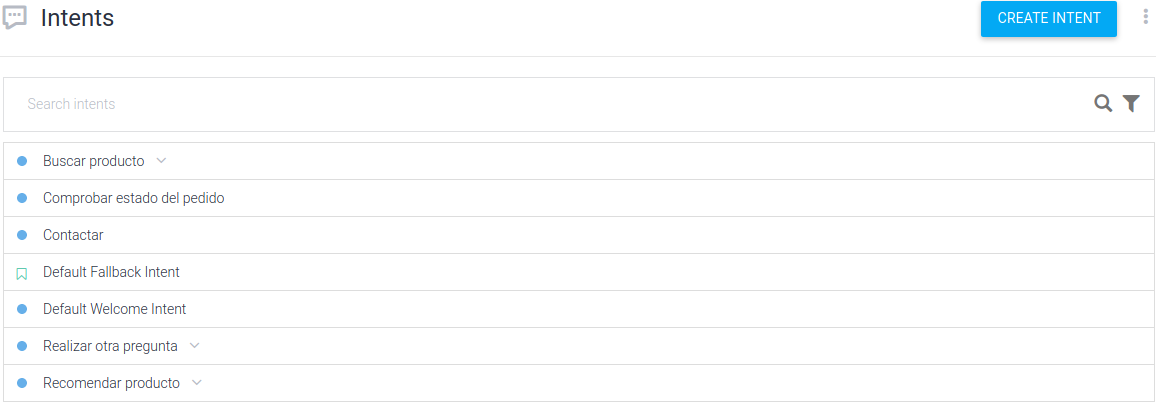
\includegraphics[width = 0.93\textwidth]{Figuras/intents.png}
	\end{center}
	\caption{\label{fig:intenciones} Intents implementados}
\end{figure}
\newpage


Para cada intent se han especificado diferentes frases de entrenamiento que actúan como ejemplo de posibles frases que los usuarios podrían escribir. Estas frases ayudan al aprendizaje del motor de lenguaje de Dialogflow. El agente no sólo intentará establecer una coincidencia con las frases registradas aquí, sino que el motor de lenguaje está continuamente aprendiendo y a partir de las frases introducidas tendrá en cuenta otras opciones. Todo esto ayuda a que el agente comprenda mejor la intención del usuario y establezca una coincidencia con el intent más apropiado. En la siguiente imagen se presentan las frases de entrenamiento usadas para configurar el intent "Realizar otra pregunta - paquete manipulado":

\begin{figure}[ht]
	\begin{center}
		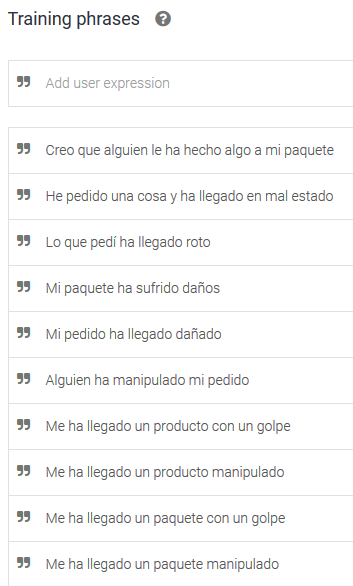
\includegraphics[width = 0.40\textwidth]{Figuras/trainingPhrases.PNG}
	\end{center}
	\caption{\label{fig:frasesEntrenamiento} Frases de entrenamiento configuradas}
\end{figure}
\newpage

Cuando el usuario realice una petición, el agente buscará la frase más parecida entre todas estas frases de entrenamiento y establecerá una coincidencia con el intent al que pertenezca dicha frase. Siguiendo con el ejemplo anterior, cuando el agente establece una coincidencia con el intent "Realizar otra pregunta - paquete manipulado" responderá como se muestra a continuación:

\begin{figure}[ht]
	\begin{center}
		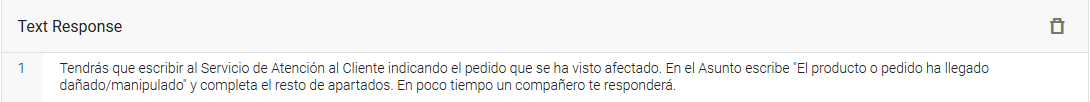
\includegraphics[width = 0.95\textwidth]{Figuras/intentResponse.PNG}
	\end{center}
	\caption{\label{fig:respuesta} Respuesta configurada}
\end{figure}

Al introducir las frases de entrenamiento, se pueden asignar una palabra o conjunto de ellas a un tipo de entidad. Estas palabras son extraídas en forma de parámetros o variables que se pueden utilizar para realizar alguna lógica u ofrecer mejores respuestas a los usuarios. Para ilustrar el funcionamiento de los parámetros, se pone como ejemplo el intent "Comprobar el estado del pedido" donde el agente recibe una petición por parte del usuario para comprobar la situación de su pedido. Cuando el agente procesa la petición, busca el número de pedido que previamente se ha establecido como un valor requerido, y si no lo encuentra se lo pedirá al cliente antes de ofrecerle la información sobre su pedido. En la siguiente imagen aparecen en color verde los caracteres que se han identificado como entidad "PedidoID":

\begin{figure}[ht]
	\begin{center}
		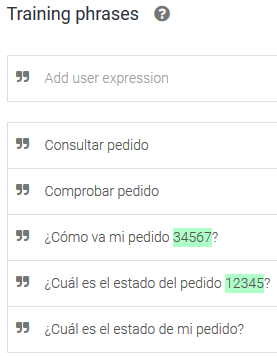
\includegraphics[width = 0.30\textwidth]{Figuras/trainingPhrasesParameters.PNG}
	\end{center}
	\caption{\label{fig:entidades} Identificación de las entidades}
\end{figure}
\newpage

Se debe especificar el parámetro o variable donde se almacenará la información correspondiente a esa entidad e indicar que es obligatorio. También es necesario configurar una respuesta para que el agente requiera al usuario la información sobre dicha entidad en caso de que no la haya proporcionado en su petición. En la figura mostrada a continuación se detalla la configuración de los parámetros para este intent:

\begin{figure}[ht]
	\begin{center}
		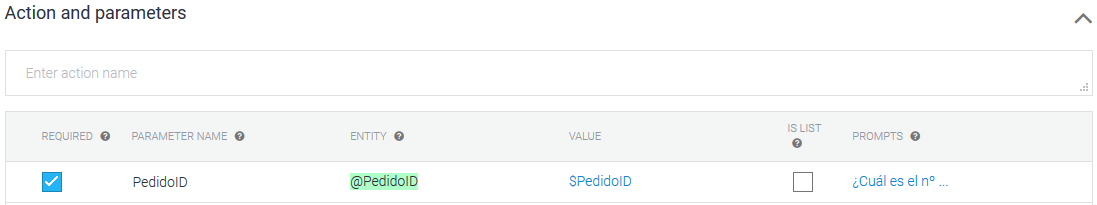
\includegraphics[width = 0.95\textwidth]{Figuras/parametersOrderID.PNG}
	\end{center}
	\caption{\label{fig:parametros} Configuración de los parámetros}
\end{figure}

Se puede indicar al agente que active un intent si se produce un determinado evento, como puede ser el caso del intent "Welcome" que se lleva a cabo cuando se abre el chat. Por ejemplo: cuando el agente no encuentra ninguna correspondencia con el registro de intents, se activa el intent "Default Fallback Intent", debido a que ha sido configurado con la entrada \textit{"input.unknown"}


Por último, es posible especificar contextos de entrada y salida que sirven para relacionar diferentes intents manteniendo información entre ellos. Cuando se produce una coincidencia con un intent, si cuenta con un contexto de salida definido se activará. Si hay contextos activos, el agente tendrá más probabilidades de establecer una coincidencia con intents que tengan definido el contexto activo como contexto de entrada. Por ejemplo: cuando se activa el intent "Buscar producto" también lo hace el contexto \textit{"Buscarproducto-followup"} que a su vez está configurado como contexto de entrada para los intents "Buscar producto - tarjetas gráficas", "Buscar producto - teclados", "Buscar producto - ratones". Por tanto, si el usuario no ha seleccionado previamente la búsqueda de un producto, entonces no se producirá una coincidencia con ninguno de estos intents. A continuación, se muestra un detalle de cómo se han configurado los contextos de entrada y salida para el intent "Buscar producto - teclados":

\begin{figure}[ht]
	\begin{center}
		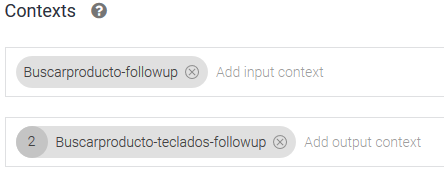
\includegraphics[width = 0.70\textwidth]{Figuras/contexts.PNG}
	\end{center}
	\caption{\label{fig:contextos} Configuración de los contextos}
\end{figure}

\newpage

\subsubsection{Entidades}

Las entidades son útiles para categorizar el contenido proporcionado por el usuario y extraer información del mismo. Dialogflow ofrece una buena cantidad de entidades predefinidas que sirven para identificar tipos de datos comunes. A pesar de ello, en este proyecto se han creado tres entidades que almacenen la información necesaria para realizar peticiones a la base de datos. Aunque actualmente el agente no está conectado a la base de datos, si que se plantea como trabajo futuro. De esta forma, se ha querido al menos sentar las bases para su posterior implementación. Las tres entidades creadas son:

\begin{itemize}
    \item \textbf{@marca}. Engloba todas las palabras para referirse a las diferentes marcas a las que pertenecen los productos que el negocio tiene en venta.
    
     \begin{figure}[ht]
    	\begin{center}
    		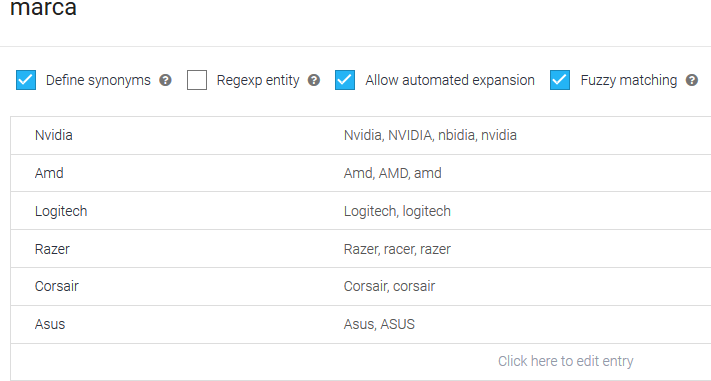
\includegraphics[width = 0.95\textwidth]{Figuras/entityMarca.PNG}
    	\end{center}
    	\caption{\label{fig:entidadMarca} Configuración de la entidad @marca}
    \end{figure}
    
    \item \textbf{@PedidoID}. Se ha definido una expresión regular para identificar los números de pedido. En este caso se trata de un número de cinco cifras comprendidas entre 0 y 9.
    
     \begin{figure}[ht]
    	\begin{center}
    		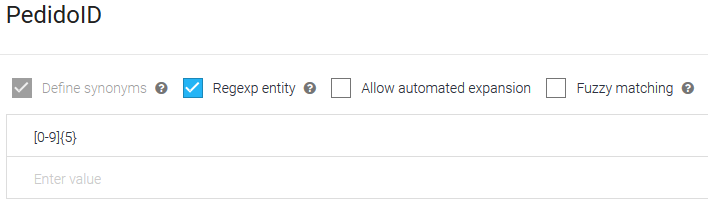
\includegraphics[width = 0.95\textwidth]{Figuras/entityPedidoID.PNG}
    	\end{center}
    	\caption{\label{fig:entidadPedido} Configuración de la entidad @PedidoID}
    \end{figure}
    
    \newpage
    
    \item \textbf{@producto}. En esta entidad se recogen los diferentes nombres con los que identificar a los productos que se venden en la página web.
    
    \begin{figure}[ht]
    	\begin{center}
    		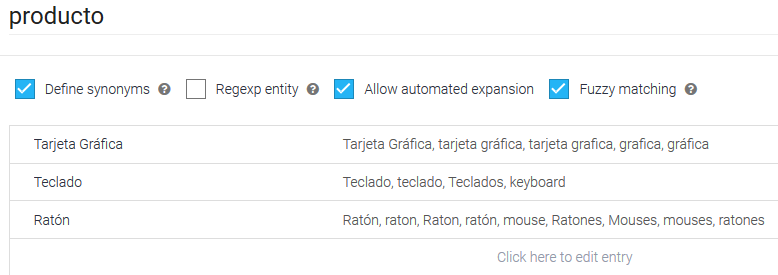
\includegraphics[width = 0.95\textwidth]{Figuras/entityProducto.PNG}
    	\end{center}
    	\caption{\label{fig:entidadProducto} Configuración de la entidad @producto}
    \end{figure}
\end{itemize}

Como se puede observar en las imágenes anteriores, para cada palabra perteneciente a una entidad se definen una serie de sinónimos que pueden ser utilizados por el usuario para referirse al mismo concepto. Además en la parte superior se encuentran las opciones "Allow automated expression" y "Fuzzy Matching". Mediante la primera opción, se activa o desactiva el aprendizaje automático del motor de lenguaje, esta capacidad permite al motor proveer nuevos sinónimos para los distintos elementos pertenecientes a la entidad. En cuanto a la segunda opción, si se activa, permite al motor extraer los parámetros que coincidan con una entidad parcialmente (en lugar de exactamente), de esta forma el motor intentará encontrar coincidencias teniendo en cuenta errores de escritura o la introducción de sólo una parte de las palabras que forman una entrada de la entidad. 

\newpage

\subsubsection{Integración}

Dialogflow se puede integrar fácilmente en un gran abanico de plataformas de conversación populares. Admite hasta 17 plataformas entre las que se encuentran Twitter, Facebook, Slack, Google Assistant, Skype, etc. También se pueden desarrollar integraciones independientes con otras plataformas haciendo uso de la API de Dialogflow, sin embargo, Google no ofrece asistencia para este tipo de integraciones.

Con el objetivo de incorporar el bot conversacional a Wordpress se ha usado MyChatbot, una extensión completamente gratuita y de instalación sencilla. Para conectar este plugin con el bot conversacional basta con copiar el token de acceso que provee Dialogflow en el campo "Access token" situado en la pestaña de configuración de MyChabot.

Dialogflow sólo permite los mensajes de respuesta enriquecida en algunas plataformas de mensajería como Slack, Skype, Facebook, etc. Con este tipo de mensajes se pueden incorporar imágenes, botones, enlaces, tarjetas, entre otras características. Por este motivo se ha desarrollado el bot usando Facebook Messenger como plataforma de mensajería. Esta decisión no supone ningún problema porque MyChatbot puede adoptar la apariencia de algunas plataformas de mensajería, simplemente dentro de las opciones de configuración se selecciona la plataforma deseada. 

En la siguiente figura se muestra cómo configurar MyChatbot:

\begin{figure}[ht]
    	\begin{center}
    		\includegraphics[width = 0.95\textwidth]{Figuras/configuracionMychatbot.png}
    	\end{center}
    	\caption{\label{fig:mychatbotConfig} Configuración del plugin MyChatbot}
\end{figure}

\newpage

\section{Despliegue}

En este sección se detalla cómo crear y desplegar los contenedores de la página web y la aplicación de análisis de sentimientos. Se dedica una subsección para explicar el proceso específico de cada proyecto, que estará estructurada de la siguiente forma:

\begin{itemize}
    \item \textbf{Modificaciones necesarias en el proyecto}. Principalmente, se deben actualizar las variables que controlan el acceso a la base de datos, debido a que se utilizará una instancia del servicio Cloud SQL. Además, en el caso de Wordpress, también se debe forzar la conexión HTTPS, ya que es el protocolo usado por Cloud Run.
    \item \textbf{Dockerfile}. Se detallará la implementación de los ficheros utilizados para la construcción de los contenedores.
    \item \textbf{Configuración del servicio en Cloud Run}. Se explicarán las opciones disponibles para configurar el servicio. Existen tres menús diferentes:
    \begin{itemize}
        \item Contenedor. Incluye las opciones de capacidad y autoescalado del contenedor, así como algunos campos generales.
        \item Variables. Aquí se establecen las variables de entorno.
        \item Conexiones. Se deben definir las conexiones de la aplicación con otros servicios de Google Cloud.
    \end{itemize}
\end{itemize}

En la siguiente imagen se muestran gráficamente los pasos que se seguirán:

\begin{figure}[ht]
    	\begin{center}
    		\includegraphics[width = 0.95\textwidth]{Figuras/Despliegue.JPG}
    	\end{center}
    	\caption{\label{fig:deployCloudRun} Pasos para crear un servicio en Cloud Run}
\end{figure}

Antes de proceder con el desarrollo específico de cada aplicación, el primer paso es configurar una instancia de MySQL en Cloud SQL que será necesaria para ambas aplicaciones.

\newpage

Este proceso es sencillo, una vez en el menú principal de Cloud SQL se selecciona "Crear Instancia" y se escoge el tipo MySQL. A continuación, se requiere introducir la información de la instancia que incluye un id de instancia, contraseña, ubicación, zona y versión de la base de datos. En la siguiente imagen se muestra dicha información:

\begin{figure}[ht]
    	\begin{center}
    		\includegraphics[width = 0.50\textwidth]{Figuras/informaciónCloudSQL.PNG}
    	\end{center}
    	\caption{\label{fig:informacionCloudSQL} Información de la instancia de Cloud SQL}
\end{figure}

Se presentan además una serie de opciones de configuración, escogiendo en su mayoría las opciones por defecto. Para este proyecto se ha seleccionado el tipo de máquina db-f1-micro, ya que con la opción más simple es suficiente. También se debe habilitar la IP pública para poder acceder a la base de datos desde diferentes equipos. A continuación, se enseñan ambos apartados de configuración:

\newpage

\begin{figure}[ht]
\begin{subfigure}{0.5\textwidth}
\includegraphics[width=0.9\linewidth, height=10cm]{Figuras/ConectividadSQL.PNG}
\caption{Conectividad Cloud SQL}
\label{fig:conectividadSQL}
\end{subfigure}
\begin{subfigure}{0.5\textwidth}
\includegraphics[width=0.9\linewidth, height=5cm]{Figuras/InstanciaCloudSQL.PNG}
\caption{Instancia Cloud SQL}
\label{fig:instanciaSQL}
\end{subfigure}

\caption{Opciones de configuración Cloud SQL}
\label{fig:configuracionCloudSQL}
\end{figure}

Una vez creada la base de datos en Cloud SQL hay que proceder a transferir los datos utilizados en el entorno local. Para ello, primero se exporta la base de datos utilizada por Wordpress desde la interfaz de phpMyAdmin. Después, haciendo uso del servicio de Cloud Storage se sube el fichero resultante de la exportación para que sea accesible al resto de servicios de Google Cloud. Por último, desde el menú "Visión General de Cloud SQL" se selecciona la opción "Importar", una vez aquí se debe elegir el archivo anterior y la base de datos donde importar la información.

\subsection{Página web}

\subsubsection{Modificaciones necesarias del proyecto local}

Como a partir de ahora se utilizará una base de datos diferente a la configurada inicialmente en local, es necesario introducir modificaciones en el archivo \textit{wp\_config}. En primer lugar se deben cambiar los campos relacionados con la conexión a la base de datos para hacer uso de variables de entorno. Sus valores se especificarán cuando se realice el despliegue del contenedor en Cloud Run.

\newpage 

\begin{lstlisting}[caption= Variables de entorno wp-config.php]
define('DB_NAME', getenv('DB_NAME'));
define('DB_USER', getenv('DB_USER'));
define('DB_PASSWORD', getenv('DB_PASSWORD'));
define('DB_HOST', getenv('DB_HOST'));
\end{lstlisting}

En segundo lugar, es necesario introducir el siguiente fragmento de código al inicio del fichero para forzar la conexión HTTPS en el área de administración (wp-admin), debido a que Cloud Run redirige todas las peticiones HTTP a HTTPS:

\begin{lstlisting}[caption= Forzar conexi\'on https]
if (
 isset($_SERVER['HTTP_X_FORWARDED_PROTO']) &&
 strpos($_SERVER['HTTP_X_FORWARDED_PROTO'], 'https') !== false
) {
 define('FORCE_SSL_ADMIN', true);
 $_SERVER['HTTPS'] = 'on';
}
\end{lstlisting}

\subsubsection{Dockerfile}

Una vez introducidas las modificaciones necesarias en los ficheros de Wordpress, se procede a crear la imagen de contenedor del proyecto que se encuentra en local. Las instrucciones para su creación se indican mediante el siguiente fichero dockerfile:

\begin{lstlisting}[caption= Dockerfile de Wordpress]
FROM wordpress:5.4.2-php7.2-apache

EXPOSE 8080

RUN sed -i 's/80/8080/g' /etc/apache2/sites-available/000-default.conf /etc/apache2/ports.conf

COPY --chown=www-data:www-data ./ /var/www/html/

WORKDIR /var/www/html/
\end{lstlisting}
 
De todas las imágenes de contenedor de Wordpress disponibles en el repositorio de docker hub, se ha seleccionado la que incluye las versiones más actualizadas de Wordpress y PHP, así como,  un servidor web que se indica mediante la etiqueta \textit{-apache}. A partir de esta imagen, se introducen algunas modificaciones para construir un contenedor propio. 

A través del comando \textit{EXPOSE 8080} se establece que éste sea el puerto de escucha utilizado por el contenedor durante su ejecución. Sin embargo, la imagen predeterminada de Apache escucha en el puerto 80, por lo tanto, se reemplaza su valor por el de 8080 utilizando el comando \textit{sed}.

Cuando la página web se encuentre en línea, su contenido será servido a través de Apache. Si se quiere introducir alguna modificación desde el panel de control de Wordpress se realizará mediante el usuario asignado a Apache, \textit{www-data}, que es diferente del usuario actual de nuestra carpeta en local. Por tanto, para evitar un error de permisos se modifica el propietario de los ficheros del proyecto en local con la instrucción \textit{--chown=www-data:www-data}. También es necesario que el contenido de la página esté disponible en el directorio de trabajo del servidor web, por ello se copia el contenido del proyecto en \textit{/var/www/html/}.

Por último, únicamente se debe establecer como directorio de trabajo el del servidor web. Esto se realiza con la instrucción \textit{WORKDIR /var/www/html/}.

Una vez que se ha creado el contenedor, el siguiente paso es subirlo a Container Registry, el servicio donde se alojan las imágenes de contenedores de forma que puedan ser usadas por el resto de servicios de Google Cloud. Los comandos que se deben ejecutar a través de la consola son los siguientes:

\begin{lstlisting}[caption= Subir imagen del contenedor a Container Registry]
docker tag <ID de la imagen> gcr.io/sentiments-analysis-263717/wordpress-server
docker push gcr.io/sentiments-analysis-263717/wordpress-server
\end{lstlisting}

donde:
\begin{itemize}
    \item gcr.io es el host de Container Registry;
    \item sentiments-analysis-263717 es el nombre del proyecto;
    \item wordpress-server es el nombre del servidor.
\end{itemize}

\subsubsection{Configuración del servicio en Cloud Run}

Tras completar esta tarea se procede a crear el servicio de Cloud Run que hará uso de dicha imagen. En primer lugar, se debe realizar la configuración del servicio indicando la región donde se ubicará el mismo, el nombre y la forma de autenticación. Es importante permitir las invocaciones sin autenticar ya que se está implementando una página web de acceso libre. La otra opción "Requerir Autenticación" hace uso de Cloud IAM, un servicio mediante el que Google permite configurar el control de acceso a través de cuentas de servicio que se utilizan para restringir las llamadas a las APIs autorizadas. 

A continuación, se pueden observar las opciones de configuración:

\begin{figure}[ht]
    	\begin{center}
    		\includegraphics[width = 0.60\textwidth]{Figuras/WordpressCloudRun1.PNG}
    	\end{center}
    	\caption{\label{fig:CloudRun1} Configurar servicio de Cloud Run. Parte I}
\end{figure}

El siguiente paso consiste en configurar el contenedor desde Cloud Run. Estas opciones se encuentran en el menú de "CONTENEDOR", cada uno de sus campos está acompañado de un breve fragmento de texto explicando su función. Aquí se debe indicar el puerto de escucha del contenedor y elegir una cuenta de servicio. Además, conviene ajustar la capacidad del contenedor en función de las necesidades del servicio que se quiere desplegar.

Es necesario otorgar los siguientes roles a la cuenta de servicio que vaya a ser utilizada para ejecutar la imagen del contenedor:
\begin{itemize}
    \item Cliente de Cloud SQL. Proporciona acceso de conectividad a Cloud SQL.
    \item Agente del servicio Cloud Run. Permite que Cloud Run acceda a los recursos gestionados.
\end{itemize}

La configuración de las cuentas de servicio se realiza en el servicio Cloud IAM. Como en este caso se ha utilizado la cuenta predeterminada del proyecto cloud, se selecciona y se añaden los roles indicados anteriormente. En la siguiente figura se muestra la cuenta de servicio y sus roles:

\begin{figure}[ht]
    	\begin{center}
    		\includegraphics[width = 0.95\textwidth]{Figuras/rolesCloudIAM.PNG}
    	\end{center}
    	\caption{\label{fig:IAM} Cuenta de servicio}
\end{figure}

Sobre la capacidad se pueden modificar los siguientes campos:
\begin{itemize}
    \item Memoria asignada. Memoria asignada a cada una de las instancias del contenedor. Acepta las unidades MiB, GiB, MB y GB.
    \item CPU asignada. Número de vCPU asignadas a cada instancia del contenedor.
    \item Tiempo de espera de solicitud. Espacio en el que espera recibir una respuesta. Se indica en segundos y el límite es de 900s.
    \item Número máximo de solicitudes por contenedor. El máximo número de peticiones que una instancia puede manejar de forma simultánea.
\end{itemize}

En cuanto al autoescalado, sólo se puede modificar el número máximo de instancias que puede crear Cloud Run en función del número de peticiones que esté recibiendo.

Seguidamente, se pueden observar los campos de configuración relacionados con la capacidad y el autoescalado:

\begin{figure}[ht]
    	\begin{center}
    		\includegraphics[width = 0.70\textwidth]{Figuras/CapacidadAutoescaladoCloudRun.PNG}
    	\end{center}
    	\caption{\label{fig:CapacidadCloudRun} Capacidad y autoescalado del contenedor en Cloud Run}
\end{figure}

\newpage

En el apartado de "VARIABLES" se deben especificar las variables de entorno utilizadas en el archivo \textit{wp\_config.php} para establecer la conexión con la base de datos. En la próxima figura se muestran las variables creadas:

\begin{figure}[ht]
    	\begin{center}
    		\includegraphics[width = 0.60\textwidth]{Figuras/VariablesCloudRun.PNG}
    	\end{center}
    	\caption{\label{fig:VariablesCloudRun} Variables de entorno Cloud Run}
\end{figure}

El campo DB\_HOST debe cumplir con el siguiente formato \textit{:/cloudsql/Nombre\_Conexión\_Instancia}. El valor de este parámetro puede ser encontrado en la pestaña "Visión General" de Cloud SQL, de la manera que se muestra:

\begin{figure}[ht]
    	\begin{center}
    		\includegraphics[width = 0.70\textwidth]{Figuras/NombreCloudSQL.PNG}
    	\end{center}
    	\caption{\label{fig:NombreCloudSQL} Nombre de conexión Cloud SQL}
\end{figure}

\newpage

Para finalizar con la configuración tan sólo falta conectar el servicio de Cloud Run con la instancia de Cloud SQL, seleccionando en el menú desplegable de la pestaña "CONEXIONES" la instancia que se va a utilizar. La próxima imagen muestra la configuración de las conexiones:

\begin{figure}[ht]
    	\begin{center}
    		\includegraphics[width = 0.55\textwidth]{Figuras/ConexionCloudSQL.PNG}
    	\end{center}
    	\caption{\label{fig:ConexionCloudSQL} Configuración de la conexión}
\end{figure}

\newpage

\subsection{Análisis de sentimientos}

\subsubsection{Modificaciones necesarias del proyecto local}

Una vez desplegada, la aplicación utilizará la misma instancia de Cloud SQL que Wordpress. Por tanto, se debe modificar la función de la aplicación que configura la forma de acceder a la base de datos. Para ello se ha introducido una variable de entorno que comprueba si se está ejecutando la aplicación en local o producción y, en función de ella, se realiza la conexión con la base de datos de un modo u otro:

\begin{lstlisting}[caption= Conexi\'on a la BBDD en funci\'on del entorno de trabajo]
    if config.IsProduction {
		var dbURI string
		dbURI = fmt.Sprintf("%s:%s@unix(/cloudsql/%s)/%s",
			config.DBConn.DBUser, config.DBConn.DBPwd, config.DBConn.InstanceConnectionName, config.DBConn.DBName)

		dbPool, err := sql.Open("mysql", dbURI)
		if err != nil {
			panic("Failed to initialize the database")
		}

		return &Connection{Conn: dbPool}
	}

	db, err := sql.Open(config.DBConn.DBDriver,
		config.DBConn.DBUser+":"+config.DBConn.DBPwd+"@/"+config.DBConn.DBName)
	if err != nil {
		panic("Failed to initialize the database")
	}

	return &Connection{Conn: db}
\end{lstlisting}

Además, la inicialización de las variables de conexión a la BBDD también se realiza teniendo en cuenta el entorno como se puede apreciar: 

\begin{lstlisting}[caption= Inicializaci\'on de variables de conexi\'on a la BBDD]
func init() {
	if mustGetenv("PRODUCTION") == "true" {
		IsProduction = true

		Key = mustGetenv("KEY")

		DBConn.DBUser = mustGetenv("DB_USER")
		DBConn.DBPwd = mustGetenv("DB_PWD")
		DBConn.InstanceConnectionName = mustGetenv("INSTANCE_CONNECTION_NAME")
		DBConn.DBName = mustGetenv("DB_NAME")
		return
	}
	DBConn.DBUser = "root"
	DBConn.DBPwd = ""
	DBConn.DBDriver = "mysql"
	DBConn.DBName = "project"
}
\end{lstlisting}

Más adelante será necesario establecer estas variables de entorno durante la configuración del servicio en Cloud Run.

\subsubsection{Dockerfile}

Tras haber realizado las modificaciones necesarias en la aplicación, se procede con la creación del contenedor. El fichero implementado es el siguiente:

\begin{lstlisting}[caption= Dockerfile an\'alisis de sentimientos]
FROM golang:1.13

ENV PORT 5002

RUN mkdir /app
WORKDIR /app/
COPY . .

RUN go mod download && \
    go install .

CMD ["code.sentiments"]
\end{lstlisting}

Con FROM se indica la imagen base para la construcción de la aplicación dentro del contenedor que, en este caso, se trata de la última versión de Go 1.13, debido a que la aplicación utiliza esta distribución.

El contenedor utilizará el puerto 5002 para comunicarse con los clientes del servicio, que se especifica creando una variable de entorno PORT.

A continuación, se crea el directorio "/app" mediante el comando RUN  - permite ejecutar un comando SHELL en el contenedor- seguido de la instrucción unix, mkdir. Esta carpeta se establece como el directorio de trabajo del contenedor con el comando WORKDIR y se copia todo el contenido de la aplicación en él utilizando COPY.

En las siguientes líneas se actualizan las dependencias del proyecto mediante "go mod download" y se crea el ejecutable de la aplicación en el directorio actual, "go install ."

Finalmente, se ejecuta el módulo de Go que identifica la aplicación. A diferencia de RUN, el comando CMD se ejecuta una vez que el contenedor se ha inicializado, en lugar de durante la creación de la imagen. Un módulo de Go es una colección de paquetes almacenados en un árbol de archivos que tienen como raíz un fichero "go.mod" donde se definen las rutas de importación así como los requisitos de dependencia.

Una vez creado el Dockerfile se construye la imagen del contenedor y se almacena en Container Registry ejecutando las siguientes instrucciones en consola:
\begin{lstlisting}[caption= Crear y subir imagen del contenedor a Container Registry]
docker build ./
docker tag <ID de la imagen> gcr.io/sentiments-analysis-263717/sentiments-server
docker push gcr.io/sentiments-analysis-263717/sentiments-server
\end{lstlisting}

donde:
\begin{itemize}
    \item gcr.io es el host de Container Registry;
    \item sentiments-analysis-263717 es el nombre del proyecto;
    \item sentiments-server es el nombre del servidor.
\end{itemize}

\subsubsection{Configuración del servicio en Cloud Run}

El proceso a seguir es el mismo que el realizado en la sección anterior para desplegar la página web. Esta vez el puerto del contenedor será el 5002 como se indica en en el Dockerfile. También se deben crear las variables de entorno propias de esta aplicación. En la siguiente figura se muestran dichas variables

\begin{figure}[ht]
    	\begin{center}
    		\includegraphics[width = 0.70\textwidth]{Figuras/variablesEntornoSentiments.PNG}
    	\end{center}
    	\caption{\label{fig:entornoSentiments} Variables de entorno para la aplicación de análisis de sentimientos}
\end{figure}

Tras completar la configuración, la aplicación estará disponible para su uso a partir de la URL ofrecida por Cloud Run.
\chapter{Conclusiones}

Con este trabajo se ha podido comprobar una manera específica de emplear la inteligencia artificial como herramienta de marketing digital en una tienda electrónica.

Gracias a la aplicación de análisis de sentimientos desarrollada se obtiene información sobre el grado de satisfacción de los clientes. Esto, ya se conseguía anteriormente cuando eran los usuarios quiénes introducían la puntuación. Sin embargo, una de las principales diferencias es que ahora la evaluación de las opiniones está normalizada, en el sentido de que Google NLP siempre utiliza el mismo conjunto de reglas.

La satisfacción del consumidor está estrechamente ligada al personal de atención, ya que es la cara visible de la empresa. Con la implementación del chatbot en la página web se ha creado un nuevo canal de atención al cliente que estará siempre disponible para responder rápidamente a los problemas de los usuarios. También consigue facilitar el uso del servicio que ofrece la tienda a través de la búsqueda y recomendación de productos. 

La tecnología utilizada refleja la importancia del Cloud Computing como agente democratizador de la IA. Sin la plataforma de Google Cloud, u otras similares,  hubiera sido imposible para un estudiante con pocos conocimientos sobre IA desarrollar un sistema como éste. Aunque es cierto que el trabajo tiene un amplio margen de mejora, como se mostrará en la sección 7.2, se ha procurado mostrar el potencial que conlleva la integración de estas aplicaciones en una tienda electrónica.

Asimismo, se ha conseguido desplegar un sitio web robusto que podrá recibir una gran cantidad de tráfico sin ver mermado su rendimiento, lo que se consigue gracias a un ajuste de escala y de capacidad automáticos. Al tratarse de un servicio completamente gestionado por el proveedor, la empresa podrá centrarse en su actividad principal y olvidarse de los aspectos técnicos relacionados con la infraestructura, flexibilidad y disponibilidad de recursos.

A pesar de estas ventajas, se ha concluido que Cloud Run no es la plataforma más indicada para alojar la página web. Este servicio ejecuta contenedores sin estado, por tanto las modificaciones que involucren al sistema de ficheros se perderán cuando se realice una nueva revisión del servicio. Se ha procurado minimizar este inconveniente utilizando Cloud Storage para el almacenamiento de los archivos multimedia. Sin embargo, esta solución no permite hacer perdurables los cambios relacionados con el código interno de Wordpress o sus plugins. Como puede ser la modificación de los enlaces permanentes, ya es necesario escribir en el fichero .htaccess.

Este aspecto, que resulta negativo para el alojamiento de la tienda, no lo es cuando se trata de la aplicación de análisis de sentimientos. Cloud Run sí es una excelente opción para desplegar servicios que pueden ser invocados mediante una API.

\section{Detalle específico de lo aprendido}

Este TFG supone el último paso de un camino que comenzó hace cuatro años y éste se espera que refleje los conocimientos que he ido adquiriendo, así como mis intereses personales. Comencé mi carrera universitaria en Ingeniería Informática atraído por el campo de la Inteligencia Artificial, así que cuando mi tutor me ofreció este proyecto, comprendí que por fin podría poner un pie dentro del mundo que anhelaba.

Este trabajo no sólo me ha servido para aprender nuevas tecnologías, también me ha ayudado en mi desarrollo personal. Nunca antes me había enfrentado a la realización de una tarea como ésta, siendo necesario para mí aprender a organizar mejor el tiempo, lidiar con la frustración y, sobre todo, ser constante.

En relación con los aspectos puramente técnicos del proyecto, expongo en los siguientes puntos los conocimientos más importantes que he adquirido:

\begin{itemize}
    \item \textbf{Cloud computing}. He aprendido a utilizar diferentes herramientas ofrecidas por Google Cloud como Cloud SQL, Cloud Run, NLP, DialogFlow, entre otras. Durante la carrera no he tenido contacto con ninguna plataforma de este tipo y me he dado cuenta de que tenía formada una idea equivocada sobre la computación en la nube. Pensaba en este campo como un conjunto de soluciones complejas que sólo estaban al alcance de personas muy capacitadas, pero nada más lejos de la realidad. Se trata de un conjunto de herramientas relativamente sencillas de utilizar, que a excepción de algunos detalles, se encuentran muy bien documentadas por parte del proveedor.
    
    \item \textbf{Contenedores}. Otro elemento con el que he trabajado por primera vez. Esta tecnología ha revolucionado la forma de implementar aplicaciones y servicios. A primera vista, para personas con experiencia en esta tecnología puede parecer sencillo el trabajo realizado, sin embargo, para mí ha supuesto un gran esfuerzo que he estado encantado de acometer.
    
    \item \textbf{APIs}. Durante la realización de mis prácticas curriculares en Altipla Consulting tuve la suerte de aprender a implementar una API utilizando gRPC y Protobuf. En este proyecto decidí utilizar un enfoque más sencillo y he aprendido a implementar una API HTTP.
    
    \item \textbf{Análisis de sentimientos}. Dados mis pocos conocimientos iniciales sobre este campo, he tenido que investigar y leer mucho acerca del mismo para realizar el trabajo. Tras finalizar, ha crecido tanto mi entendimiento como interés por esta área.
    
    \item \textbf{Interfaces conversacionales}. Me recuerdo a mí mismo durante mi segundo año de carrera manteniendo una conversación con Eliza en MS DOS. Para mí fue una experiencia muy enriquecedora y que me gustó mucho. Por ese entonces no conocía nada sobre el funcionamiento de un motor conversacional, pero gracias al pequeño chatbot que he creado haciendo uso de Dialogflow he aprendido mucho sobre esta tecnología.
\end{itemize}


La idea más importante que he adquirido y quiero resaltar es la necesidad de comunicar de forma clara y precisa el trabajo y la investigación realizados, es decir, entender que la comunicación es un aspecto fundamental. 

\section{Trabajo futuro}

En primer lugar, sobre la herramienta de análisis de sentimientos desarrollada, sería conveniente ajustar más la evaluación de las opiniones. Se puede tener en cuenta el parámetro "Magnitud" para eliminar posibles ambigüedades que se produzcan y representar de forma más precisa la valoración del usuario. Si una frase es evaluada con una puntuación cercana a cero puede ser porque posee poca intensidad o presenta emociones mixtas. En estas situaciones se puede utilizar la magnitud para eliminar la ambigüedad, ya que si realmente la frase es neutral, ésta tendrá asociada un valor de magnitud bajo. 

En segundo lugar, en cuanto a la interfaz conversacional, aún le queda un gran camino para ser una herramienta de calidad que resulte de utilidad a los clientes. Sería adecuado ahondar mucho más en sus funcionalidades. El primer paso consistiría en conectar el bot conversacional con la base de datos de la página web, consiguiendo que éste pueda buscar y recomendar productos para el cliente en base a diferentes parámetros, como el precio, la marca, su valoración media, etc. También se podrían incluir muchas más frases para interactuar con el agente hasta poder convertirlo en un verdadero empleado del Servicio de Atención al Cliente. Automatizar un proceso de negocio complejo, como puede ser la atención al cliente, es una tarea complicada que puede considerarse como el objeto de un trabajo de fin de estudios en sí misma.

En tercer lugar, el método de autenticación utilizado por la aplicación de análisis de sentimientos es muy simple. Consiste en añadir un token a las peticiones realizadas al servicio. Con el objetivo de mejorar la seguridad se plantea utilizar el servicio Firebase Authentication para implementar un modo de acceso basado en usuario y contraseña. Al tratarse de un sistema completamente gestionado por Google se conseguiría una mayor seguridad y mejor protección de los datos.

En cuarto lugar, como se ha mencionado al comienzo de este capítulo Cloud Run no es la plataforma más apropiada para desplegar la página web. Google Cloud cuenta con otras alternativas como GKE (Google Kubernetes Engine) y plataformas como Microsoft, Amazon o IBM también ofrecen servicios similares. Se debería estudiar más a fondo todas las opciones disponibles para determinar cuál es la opción que mejor se ajusta a las necesidades de un sitio web.

Por último, es importante encontrar formas de trasferir el conocimiento adquirido a las empresas donde pueda resultar de utilidad. Especialmente, es crucial insistir al tejido empresarial de las zonas rurales de Almería sobre la necesidad de acometer un proceso de transformación digital, poniendo a su disposición herramientas como las desarrolladas con este trabajo.

\addcontentsline{toc}{chapter}{Bibliografía }
\bibliographystyle{IEEEtran}
\bibliography{referencias}

\addcontentsline{toc}{chapter}{Webgrafía }
\bibliographystyleW{IEEEtran}
\bibliographyW{webs}

\appendix

\input{apendices}

\clearpage
\backmatter


\thispagestyle{empty}
%\put(0,0){
\begin{minipage}[h]{0.9\paperwidth}
\thispagestyle{empty}
\begin{tikzpicture}[remember picture,overlay]
\node (f) [rectangle]  
at (current page.center)
          {\parbox[b][\paperheight]{\paperwidth}{
           \includegraphics[width=\paperwidth,height=\paperheight,keepaspectratio]{Figuras/logos/TFG_back}
          }};
\node (texto) [rectangle,text width=0.5\paperwidth,yshift=50pt] 
at (f)
          {\parbox{0.65\paperwidth}{\justifying \Large \color{white}
         
\normalsize {}	
Actualmente, las organizaciones comienzan a implementar un nuevo modelo de marketing
centrado en las relaciones entre la empresa y sus clientes. La inteligencia artificial ha encontrado aquí un extraordinario campo de aplicación, tanto en la gestión de la información, como en la atención al cliente y el análisis de la experiencia de compra.

El proyecto desarrollado en el presente trabajo se sitúa en este contexto. Se estudian e implementan dos servicios de inteligencia artificial en una tienda electrónica. Por un lado, se construye una aplicación basada en Google Natural Language que realiza un análisis de sentimientos de los comentarios de los clientes, proporcionando una medida normalizada de su grado de satisfacción sobre el servicio ofrecido. Por otro lado, se desarrolla un agente virtual utilizando Dialogflow para ayudar al servicio de atención al cliente, automatizando las tareas más sencillas.

El sistema de software implementado se despliega a través de contenedores en Cloud Run, una plataforma sin servidor que permite a las organizaciones abstraerse de cuestiones técnicas relacionadas con la infraestructura, flexibilidad y disponibilidad de recursos.

\vspace{.5cm}

Palabras clave: Comercio electrónico, machine learning, chatbots, computación en la nube, análisis de sentimientos.

\vspace{1cm}

\newpage
 
%\section*{Abstract}

Nowadays, corporations are beginning to implement a new marketing that pays closer attention to their relationship with clients. In this area, Artificial Intelligence has found new fields of application such as data management, customer service or shopping experience analysis.

The project developed in the current work is situated in this context. Two AI services have been studied and implemented in an e-commerce. First of all, an app based on Google Natural Language has been built, it will carry out a sentiment analysis of customer feedback, providing a standardized measure of the satisfaction degree about the service offered. Second, a virtual agent has been developed using Dialogflow to help customer service by automating simple tasks.

To conclude, the system is deployed through containers on Cloud Run, a serverless platform that allows organizations to abstract from technical issues related to infrastructure, flexibility, and resource availability.

\vspace{.5cm}

Keywords: E-commerce, machine learning, chatbots, cloud computing, sentiment analysis.

         }};
       \node  at (14,-25.55) {\Large\curso};
  \end{tikzpicture}
\end{minipage}
%}


          
          

\end{document}

